\documentclass[a4paper,12pt]{report}

% Pacchetti
\usepackage[utf8]{inputenc}
\usepackage[T1]{fontenc}
\usepackage[italian]{babel}
\usepackage{amsmath,amssymb,amsfonts}
\usepackage{graphicx}
\usepackage{csquotes}
\usepackage{float}
\usepackage{caption}
\usepackage{booktabs}
\usepackage{listings}
\usepackage{tikz}
\usepackage{enumitem}
\usepackage{tabularx}
\usepackage{theorem}
\usepackage{booktabs}
\usepackage{newpxtext}
\usepackage{newpxmath}
\usepackage{microtype}
\usepackage{setspace}
\onehalfspacing
\usepackage{hyperref}

\begin{document}
	
	\begin{titlepage}
		\begin{center}
			
\includegraphics[width=0.6\textwidth]{img/logo_unibo.png}
		\end{center}
		\begin{center}
			\vspace{2cm}
			\textbf{CORSO DI LAUREA IN INGEGNERIA E SCIENZE INFORMATICHE}
			
			\vspace{2cm}
			\textbf{\Large Valutazione Metodologica ed Applicativa di KAN, MLP, Random Forest e XGBoost con Tecniche di Ottimizzazione su differenti casi di studio}
			
			\vspace{2cm}
			\begin{tabular}{p{0.8\textwidth} p{0.8\textwidth}}
				\textbf{Relatore:} & \textbf{Presentata da:} \\
				\textbf{Prof. Damiana Lazzaro} & \textbf{Martin Tomassi} \\
			\end{tabular}
			
			\vspace{2cm}
			\textbf{Sessione Settembre 2025} \\
			\textbf{Anno Accademico 2024/2025}
		\end{center}
	\end{titlepage}
	
	\tableofcontents
	
	\chapter*{Introduzione}
	% To Be Modified
	La presente tesi si propone di analizzare, confrontare e valutare diverse architetture di Machine e Deep learning: le Kolmogorov–Arnold Networks (KAN), i Multi-Layer Perceptron (MLP), le Random forest e XGBoost. \\
	L’obiettivo principale è quello di fornire, da un lato, un’analisi teorica esaustiva di ciascun modello, includendo i fondamenti matematici e le architetture; dall’altro, valutare sperimentalmente le prestazioni dei modelli su tre casi di studio: regressione sulle emissioni di automobili, classificazione dell’inquinamento atmosferico (PM2.5) e riconoscimento di immagini mediante CNN abbinate a MLP e KAN. \\
	Oltre allo studio comparativo dei modelli, la tesi include un’ampia indagine sui metodi di Hyperparameter Tuning: Grid search, Random search, Bayesian optimization e Genetic algorithms, selezionati in base ad uno studio preliminare di confronto. \\
	A completamento, sono stati condotti due studi di ablazione post-training per ogni caso di studio:
	\begin{itemize}
		\item \textbf{L1 Pruning} per KAN e MLP.
		\item \textbf{Ensemble Pruning} dove:
		\begin{itemize}
			\item \textbf{Rank-Based Pruning} per Random forest.
			\item \textbf{Cumulative Pruning} per XGBoost.
		\end{itemize}
	\end{itemize}
	
	\chapter{Multi-Layer Perceptron (MLP)}
	
	\section{Introduzione}
	Questo capitolo presenta una descrizione del Multi-Layer Perceptron (MLP), un'architettura fondamentale delle reti neurali. L'obiettivo è esplorare la sua struttura e le sue capacità di modellare relazioni complesse, a partire dai principi matematici. Verranno analizzate le sue componenti principali, tra cui la distinzione tra gli strati e le funzioni di attivazione, che sono cruciali per l'apprendimento di relazioni non lineari. Il testo spiegherà poi il meccanismo attraverso cui la rete impara, descrivendo i passaggi di calcolo che avvengono durante il forward pass e l'algoritmo di backpropagation che aggiorna i parametri del modello. Verranno inoltre affrontate le tecniche di regolarizzazione, indispensabili per evitare che la rete memorizzi i dati di addestramento invece di imparare a generalizzare. Infine, il capitolo riassume i vantaggi ed i limiti delle MLP, ponendo l'accento sulla loro flessibilità e sui problemi legati alla profondità della rete, come il vanishing/exploding gradient. \cite{popescu2009mlp, hornick1988mfn, cybenko1989uat, leshno1993uat, henseler1995back, srivastava2014dropout, schmidhuber2015deep}
	
	\begin{figure}[H]
		\centering
		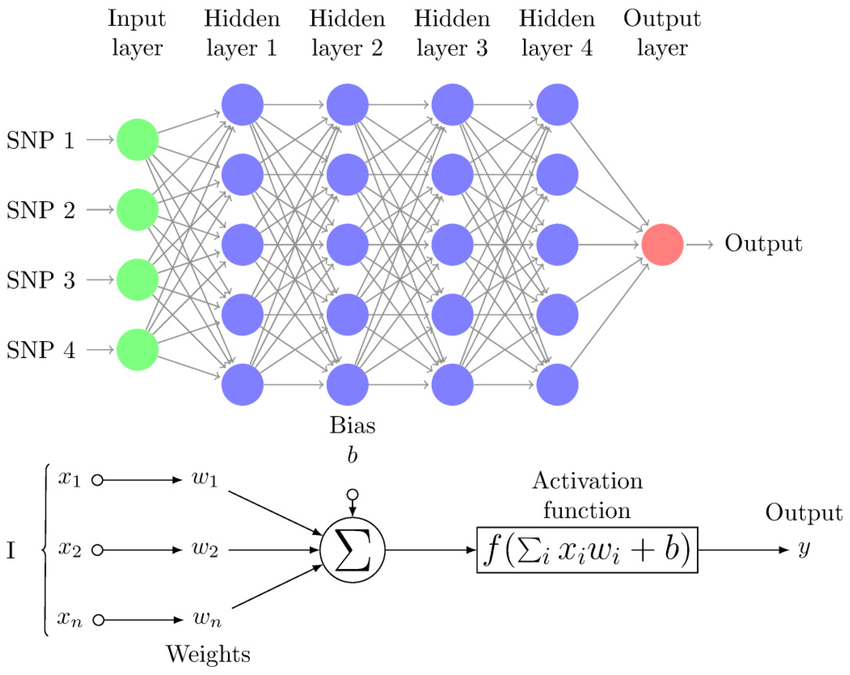
\includegraphics[width=0.8\textwidth]{img/mlp.png}
		\caption{Architettura della rete neurale Multi-Layer Perceptron.}
	\end{figure}
	
	\section{Fondamenti matematici}
	
	\subsection{Enunciato formale}
	Sia \(K\subset\mathbb{R}^n\) uno spazio compatto e sia \(C(K)\) lo spazio delle funzioni continue su \(K\) munito della norma uniforme \(\|\cdot\|_\infty\). Sia \(\sigma:\mathbb{R}\to\mathbb{R}\) una funzione di attivazione che soddisfa una delle seguenti ipotesi:
	
	\begin{enumerate}
		\item[\((A_1)\)] \(\sigma\) è continua e sigmoide, cioè \(\lim_{t\to -\infty}\sigma(t)=a\) e \(\lim_{t\to +\infty}\sigma(t)=b\) con \(a\neq b\) (Cybenko);
		\item[\((A_2)\)] \(\sigma\) è continua e non polinomiale (Leshno et\,al.). 
	\end{enumerate}
	
	Allora vale il seguente risultato di approssimazione universale.
	
	\subsection{Teorema di approssimazione universale}
	Per ogni \(f\in C(K)\) e per ogni \(\varepsilon>0\), esistono un intero \(N\in\mathbb{N}\) (indica il numero di neuroni nello strato nascosto), coefficienti scalari \(c_i\in\mathbb{R}\), vettori \(w_i\in\mathbb{R}^n\) e bias \(b_i\in\mathbb{R}\) tali che la funzione a singolo strato
	\[
	\hat f_N(x) \;=\; \sum_{i=1}^N c_i\,\sigma\bigl(w_i\cdot x + b_i\bigr)
	\]
	soddisfa
	\[
	\|f - \hat f_N\|_\infty \;=\; \sup_{x\in K} \bigl|f(x)-\hat f_N(x)\bigr| \;<\; \varepsilon.
	\]
	In altre parole, lo span delle funzioni elementari (cioè l'insieme di tutte le possibili combinazioni lineari di queste funzioni) \(x\mapsto\sigma(w\cdot x + b)\) è denso in \(C(K)\) rispetto alla norma uniforme. Ciò significa che per ogni funzione continua \(f\in C(K)\) e per ogni \(\varepsilon>0\) esiste una combinazione lineare finita di blocchi attivati da \(\sigma\) (cioè una rete a singolo strato nascosto) che approssima \(f\) uniformemente su \(K\) con errore massimo minore di \(\varepsilon\). Formalmente, la chiusura (nell'\(\|\cdot\|_\infty\)) dello spazio generato dalle funzioni elementari coincide con l'intero \(C(K)\).
	
	\subsection{Significato di \(\sup_{x\in K}\).}
	La notazione \(\sup_{x\in K}\) denota l'estremo superiore di un insieme di reali. Nella norma uniforme
	\[
	\|f-\hat f_N\|_\infty=\sup_{x\in K}|f(x)-\hat f_N(x)|
	\]
	il valore indicato è l'errore massimo di approssimazione su tutto il dominio \(K\). Poiché nel teorema \(K\) è assunto compatto e la funzione \(x\mapsto|f(x)-\hat f_N(x)|\) è continua, l'estremo superiore coincide con il massimo:
	\[
	\sup_{x\in K}|f(x)-\hat f_N(x)|=\max_{x\in K}|f(x)-\hat f_N(x)|.
	\]
	
	\paragraph{Esempio} Se \(K=[0,1]\) e \(f(x)=\sin(2\pi x)\), affermare che esiste \(N\) tale che
	\[
	\sup_{x\in[0,1]}|f(x)-\hat f_N(x)|<0.01
	\]
	significa che con quel numero di neuroni si può costruire \(\hat f_N\) che differisce dalla sinusoide al più di \(0.01\) in ogni punto dell'intervallo \([0,1]\).
	
	\subsection{Ipotesi e Precisazioni}
	\begin{itemize}
		\item \textbf{Compattezza del dominio \(K\).} Il teorema è enunciato per funzioni continue definite su un insieme compatto \(K\subset\mathbb{R}^n\) (ad es.\ l'intervallo chiuso \([0,1]^n\)). La compattezza garantisce che la norma uniforme \(\|g\|_\infty=\sup_{x\in K}|g(x)|\) sia ben definita e che l'estremo superiore sia effettivamente un massimo raggiunto su \(K\). Su domini non limitati (per es.\ \(\mathbb{R}^n\)) la formulazione uniforme non è direttamente applicabile.
		
		\item \textbf{Ipotesi sulla funzione di attivazione \(\sigma\):} la validità del risultato dipende dalle proprietà di \(\sigma\). Due formulazioni tipiche sono:
		\begin{itemize}
			\item \textbf{Sigmoide limitata e continua (Cybenko):} dove \(\sigma\) ha limiti finiti agli estremi e cambia valore tra \(-\infty\) e \(+\infty\).
			\item \textbf{Funzione continua non polinomiale (Leshno et\,al.):} condizione più generale che garantisce densità dello span.
		\end{itemize}
		Queste ipotesi escludono funzioni che non introducono la non linearità richiesta per generare uno spazio denso in \(C(K)\). Per attivazioni moderne (ad esempio, ReLU) il teorema rimane valido ma con enunciati e ipotesi tecniche differenti.
		
		\item \textbf{Natura esistenziale del risultato:} il teorema è di tipo qualitativo: afferma che esiste un numero finito di neuroni \(N\) e parametri \((c_i,w_i,b_i)\) tali che l'approssimazione uniforme è ottenuta entro qualsiasi tolleranza prefissata \(\varepsilon\). Non fornisce però una procedura esplicita per la ricerca dei parametri ed un bound quantitativo generale che esprima \(N\) in funzione di \(\varepsilon\) per una data \(f\).
		
		\item \textbf{Non implica una fase di training facile:} anche se esiste una rete che approssima \(f\), nella pratica:
		\begin{itemize}
			\item gli algoritmi numerici di ottimizzazione (SGD, Adam, ecc.) non sono garantiti a trovare quei parametri ottimali: la funzione di perdita è non convessa e può avere molteplici ottimi locali o regioni piatte;
			\item la buona approssimazione teorica non assicura buona generalizzazione se i dati a disposizione sono scarsi: quindi é necessario usare tecniche di regolarizzazione, validazione e controllo dell'overfitting.
		\end{itemize}
	\end{itemize}
	
	\section{Struttura delle MLP}
	
	\subsection{Strati: input, nascosti, output}
	Le Multi-layer Perceptron (MLP) sono una tipologia di reti neurali feed-forward, costituite da più strati (layer) di neuroni: uno strato di input, che riceve i dati iniziali; uno o più strati nascosti; ed uno strato di output che genera le previsioni finali. Ogni neurone, appartenente ad uno strato, è connesso a tutti i neuroni di quello successivo (architettura fully connected). Questo significa che ogni input viene trasformato dallo strato di input ai layer nascosti intermedi ed infine allo strato di output, con ogni collegamento caratterizzato da un peso $w$. Il numero di neuroni, in ciascun layer, è un iperparametro da scegliere: tipicamente lo strato di input ha tante unità quanti sono i parametri in ingresso, gli strati nascosti possono variare da pochi a molti nodi, a seconda del problema, e lo strato di output ha un neurone per ogni valore target. \\
	In ogni neurone (esclusi quelli di input), si calcola una somma pesata degli input e di un termine di bias, per poi applicare una funzione di attivazione. L'output di un neurone $i$ nel layer $l$ è dato da:
	$$z_i^{(l)} = \sum_{j=1}^{N_{l-1}} w_{ij}^{(l)} a_j^{(l-1)} + b_i^{(l)}$$
	$$a_i^{(l)} = \sigma(z_i^{(l)})$$
	Dove $z_i^{(l)}$ è la somma pesata, $w_{ij}^{(l)}$ è il peso della connessione, $a_j^{(l-1)}$ è l'output del neurone precedente, $b_i^{(l)}$ è il bias, e $\sigma$ è la funzione di attivazione non lineare.
	
	\subsection{Funzioni di attivazione comuni}
	Le funzioni di attivazione sono cruciali nelle reti neurali, poiché introducono la non linearità necessaria per modellare relazioni complesse tra input e output. In assenza di tali funzioni, una rete multi-layer si ridurrebbe ad una trasformazione lineare. Di seguito vengono descritte alcune delle funzioni di attivazione più diffuse, con le loro proprietà matematiche, i pro e contro.
	
	\paragraph{Proprietà rilevanti}
	Quando si valuta una funzione di attivazione, conviene considerare la sua \textbf{differenziabilità}, che è fondamentale per la backpropagation; la \textbf{boundedness dell'output e zero-centering}, cioè se l'output è centrato attorno a 0; la \textbf{saturazione}, che può causare il \textit{vanishing gradient}; la \textbf{sparsità} ed il \textbf{costo computazionale}.
	
	\subsubsection{1. Sigmoide}
	\begin{figure}[H]
		\centering
		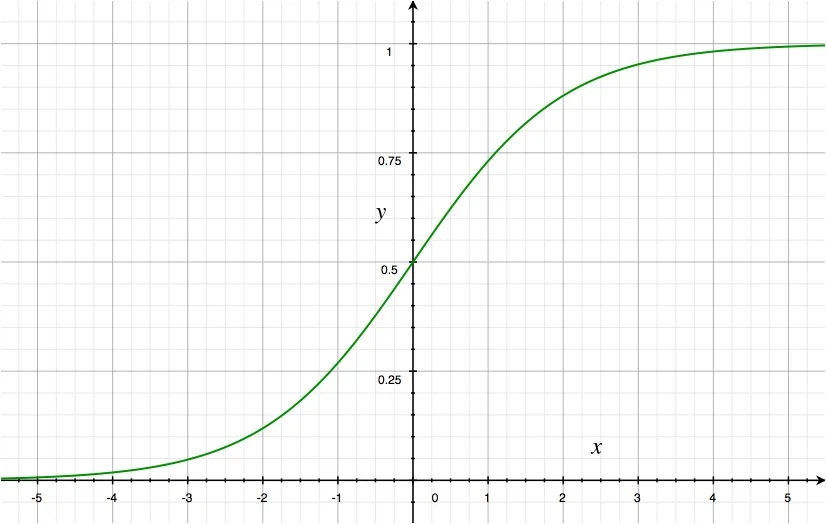
\includegraphics[width=0.8\textwidth]{img/sigmoid.png}
		\caption{Grafico della funzione di attivazione Sigmoide.}
	\end{figure}
	\[
	\sigma(x) = \frac{1}{1+e^{-x}},\qquad
	\sigma'(x)=\sigma(x)(1-\sigma(x)).
	\]
	Questa funzione ha un output che si colloca nell'intervallo $(0,1)$ ed una caratteristica forma a "S", rendendola utile per rappresentare la probabilità (quindi un output normalizzato); la sua derivata è semplice da calcolare. Tuttavia, la sua principale debolezza è la saturazione per $x\to\pm\infty$, dove il gradiente tende a zero. Questo fenomeno porta al problema del vanishing gradient nei layer profondi. È tipicamente utilizzata nello strato di output per la classificazione binaria, in combinazione con la binary cross-entropy.
	
	\subsubsection{2. Tangente iperbolica (tanh)}
	\begin{figure}[H]
		\centering
		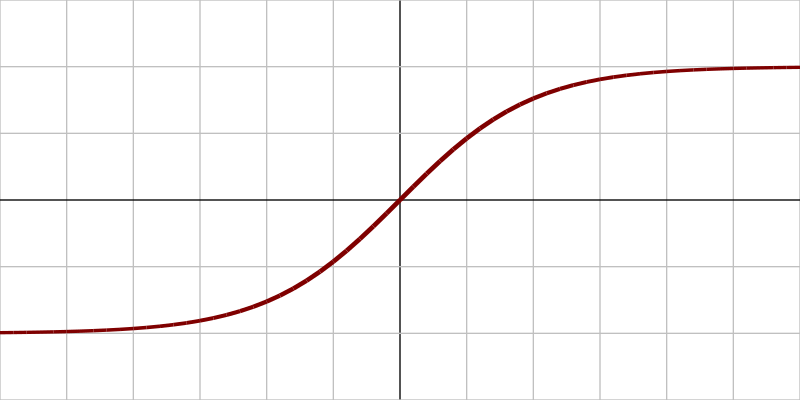
\includegraphics[width=0.8\textwidth]{img/tanh.png}
		\caption{Grafico della funzione di attivazione Tangente iperbolica.}
	\end{figure}
	\[
	\tanh(x)=\frac{e^x-e^{-x}}{e^x+e^{-x}},\qquad
	\tanh'(x)=1-\tanh^2(x).
	\]
	La funzione tanh ha un output compreso tra $(-1,1)$ ed è centrata in $0$, il che, quando i dati sono normalizzati, porta ad una convergenza migliore rispetto alla sigmoide. Nonostante questo vantaggio, rimane una funzione saturante per valori estremi, e di conseguenza può soffrire ancora del problema del vanishing gradient. Il suo uso tipico è nei layer nascosti di reti poco profonde o quando è desiderabile un output centrato.
	
	\subsubsection{3. Rectified Linear Unit ReLU (ReLU)}
	\begin{figure}[H]
		\centering
		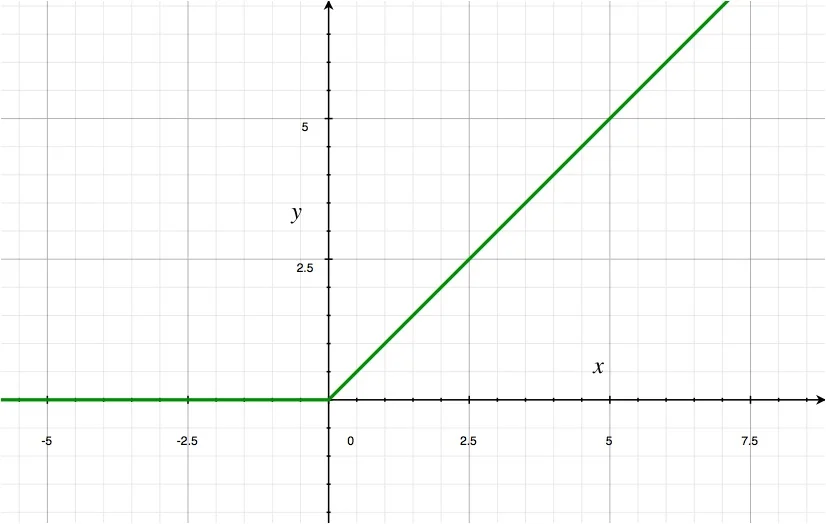
\includegraphics[width=0.8\textwidth]{img/relu.png}
		\caption{Grafico della funzione di attivazione ReLU.}
	\end{figure}
	\[
	\mathrm{ReLU}(x)=\max(0,x),\qquad
	\mathrm{ReLU}'(x)=\begin{cases}0 & x<0,\\ 1 & x>0,\end{cases}
	\]
	La ReLU è una funzione semplice e computazionalmente efficiente, che, nella maggior parte dei casi, evita il problema del vanishing gradient sulle porzioni attive e favorisce la sparsità delle attivazioni. Il principale svantaggio è il problema della "dying ReLU": i neuroni possono diventare permanentemente inattivi se ricevono input negativi. Un neurone si considera "morto" se, per tutte (o quasi) le istanze del dataset, l'input $x \le 0$, dato che in tal caso l'output è sempre nullo. Poiché la derivata di ReLU è zero per $x<0$, il gradiente non si propaga a ritroso, e il neurone non riceve più aggiornamenti dei pesi, rimanendo inattivo per tutta la durata dell'allenamento. Viene ampiamente utilizzata nei layer nascosti in quasi tutte le architetture di reti neurali.
	
	\subsubsection{4. Leaky ReLU (LReLU) / Parametric ReLU (PReLU)}
	\begin{figure}[H]
		\centering
		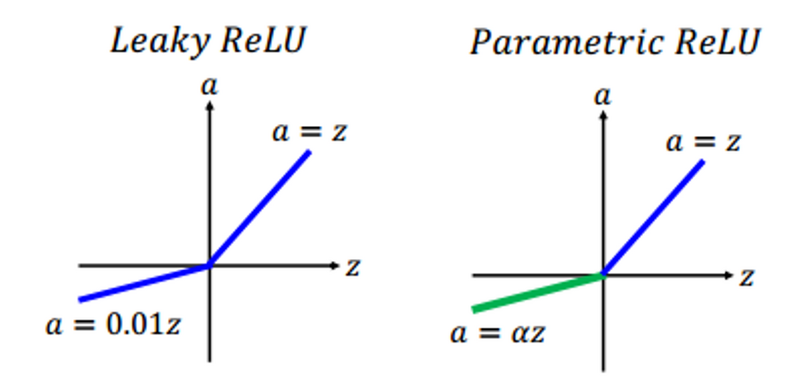
\includegraphics[width=0.8\textwidth]{img/lprelu.png}
		\caption{Grafico delle funzioni di attivazione LReLU e PReLU.}
	\end{figure}
	\[
	\mathrm{LReLU}(x)=\begin{cases}0.01x & x\le0,\\ x & x>0,\end{cases}\qquad
	\mathrm{LReLU}'(x)=\begin{cases}0.01 & x<0,\\ 1 & x>0,\end{cases}\qquad
	\]
	\[
	\mathrm{PReLU}(x)=\begin{cases}\alpha x & x<0,\\ x & x\ge0,\end{cases}\qquad
	\mathrm{PReLU}'(x)=\begin{cases}\alpha & x<0,\\ 1 & x>0,\end{cases}\qquad \alpha\in(0,1)
	\]
	PReLU apprende il parametro $\alpha$ durante il training. Entrambe le varianti mantengono un piccolo gradiente per $x<0$, riducendo significativamente il problema dei "dead neurons". L'introduzione (o l'apprendimento) di un iperparametro è un potenziale svantaggio, ed il loro comportamento non è sempre superiore a quello della semplice ReLU. Sono impiegate dove si vuole evitare il problema della "dying ReLU", mantenendo la semplicità.
	
	\subsubsection{5. Exponential Linear Unit (ELU)}
	\begin{figure}[H]
		\centering
		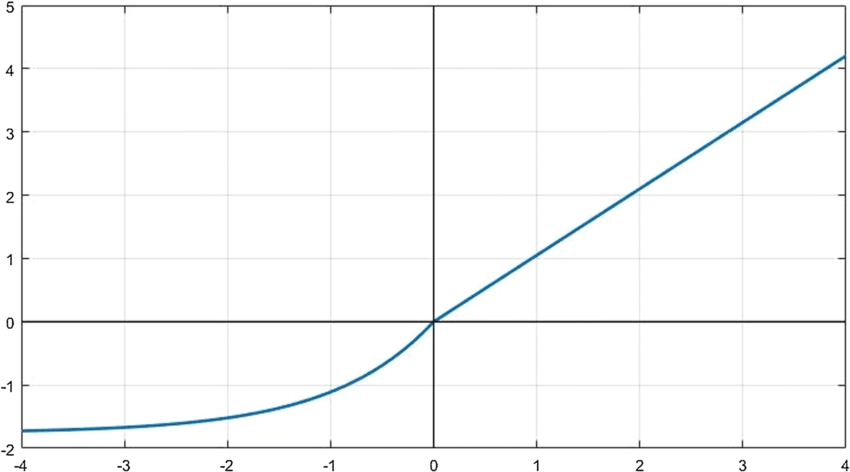
\includegraphics[width=0.8\textwidth]{img/elu.png}
		\caption{Grafico della funzione di attivazione ELU.}
	\end{figure}
	\[
	\mathrm{ELU}(x)=\begin{cases}x & x\ge0,\\ \alpha(e^x-1) & x<0,\end{cases}\qquad
	\mathrm{ELU}'(x)=\begin{cases}\alpha(e^x) & x<0,\\ 1 & x>0,\end{cases}\qquad \alpha>0
	\]
	L'ELU produce un output più centrato rispetto alla ReLU e ha un gradiente non nullo per $x<0$, che in alcuni casi può portare a una migliore convergenza. Tuttavia, è leggermente più costosa a livello computazionale a causa della funzione esponenziale ed introduce un parametro $\alpha$ da ottimizzare.
	
	\subsubsection{6. Softplus}
	\begin{figure}[H]
		\centering
		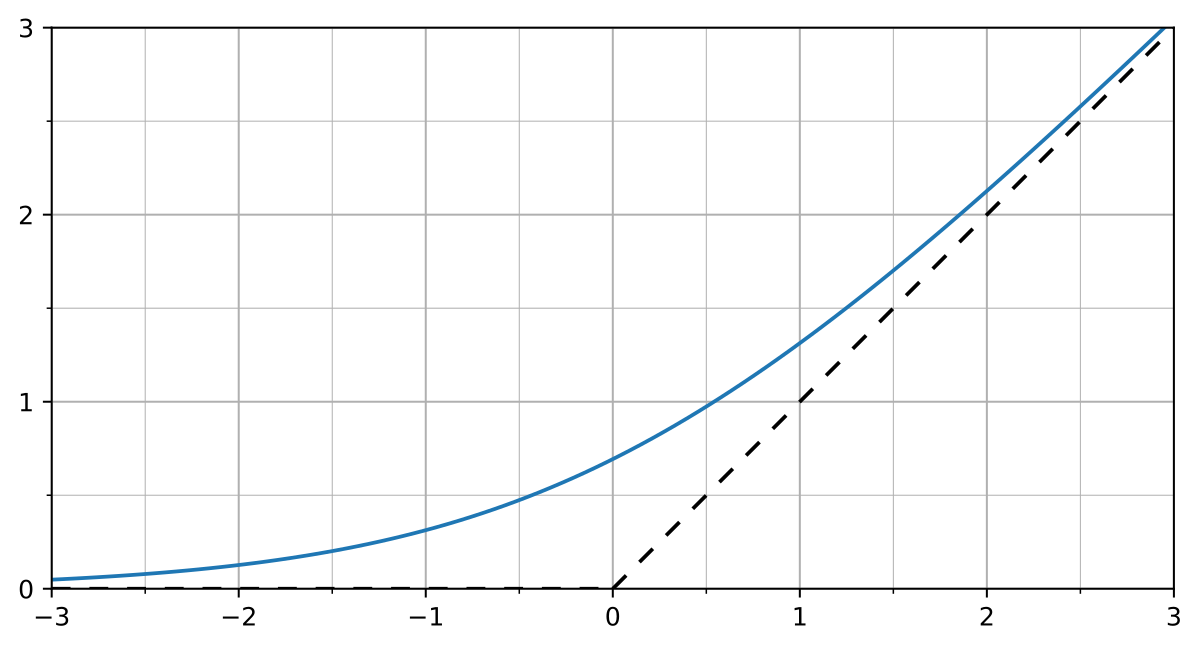
\includegraphics[width=0.8\textwidth]{img/softplus.png}
		\caption{Grafico della funzione di attivazione Softplus.}
	\end{figure}
	\[
	\mathrm{softplus}(x)=\log(1+e^x),\qquad
	\mathrm{softplus}'(x)=\frac{1}{1+e^{-x}}\qquad
	\]
	La Softplus è una versione continua e completamente differenziabile della ReLU. Nonostante questa proprietà, è più costosa dal punto di vista computazionale e meno sparsa rispetto alla ReLU.
	
	\subsubsection{7. Gaussian Error Linear Unit (GELU)}
	\begin{figure}[H]
		\centering
		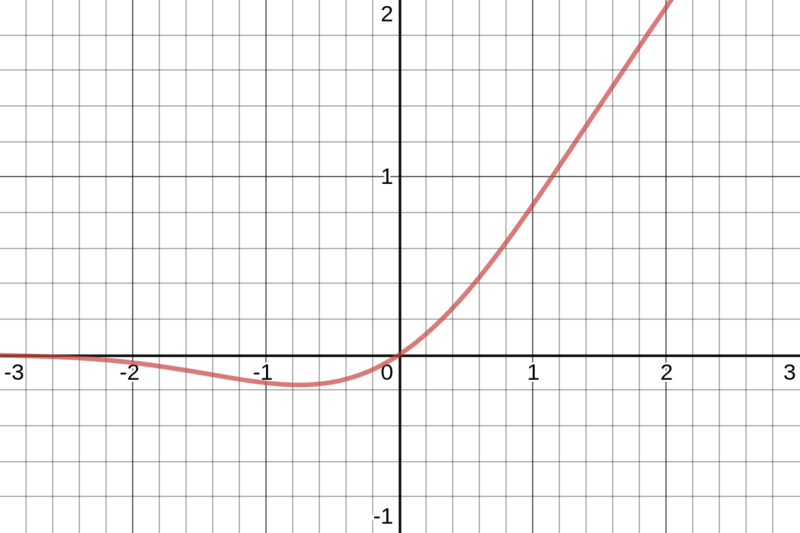
\includegraphics[width=0.8\textwidth]{img/gelu.png}
		\caption{Grafico della funzione di attivazione GELU.}
	\end{figure}
	\[
	\mathrm{GELU}(x) = x \cdot \Phi(x)
	\]
	dove $\Phi(x)$ è la funzione di distribuzione cumulativa (CDF) della distribuzione normale standard e '$\operatorname{erf}$' è la funzione degli errori di Gauss:
	\[
	\Phi(x) = \frac{1}{2} \left[ 1 + \operatorname{erf} \left( \frac{x}{\sqrt{2}} \right) \right] \qquad
	\]
	\[
	\mathrm{GELU}'(x) = \Phi(x) + \frac{1}{2}x\,\phi(x)
	\]
	dove
	\[
	\phi(x) = \frac{1}{\sqrt{2\pi}}\,e^{-x^{2}/2} \qquad
	\]
	La GELU ha dimostrato un eccellente comportamento empirico, specialmente nei modelli di linguaggio, ed è considerata una funzione di attivazione "soft" che combina linearità e gating stocastico. Il suo principale svantaggio è il costo computazionale più elevato. Viene ampiamente utilizzata nelle architetture Transformer.
	
	\subsubsection{8. Softmax}
	Per un vettore $x\in\mathbb{R}^K$:
	\[
	\mathrm{softmax}(x)_j=\frac{e^{x_j}}{\sum_{k=1}^K e^{x_k}}.
	\]
	Questa funzione viene utilizzata per trasformare i logits (gli output grezzi di un layer) in una distribuzione di probabilità. È normalmente combinata con la funzione di perdita di categorical cross-entropy per problemi di classificazione multi-classe.
	
	\section{Procedura di forward pass}
	
	\subsection{Calcolo delle attivazioni}
	Durante la fase di propagazione in avanti (forward pass), i dati attraversano la rete dallo strato di input a quello di output. Ogni neurone calcola prima un ingresso pesato sommandolo con il bias. Dato un neurone $j$ dello strato nascosto o di output, l'eccitazione, o attivazione lineare, è:
	\[
	z_j = \sum_i w_{ji} x_i + b_j,
	\]
	dove $x_i$ sono gli output (o input iniziali), $w_{ji}$ i pesi di connessione, e $b_j$ il bias. In seconda battuta, si applica la funzione di attivazione $\phi$ per ottenere l'uscita del neurone:
	\[
	a_j = \phi(z_j).
	\]
	Ad esempio, con $\phi=\sigma$ (sigmoide), avremmo $a_j=1/(1+e^{-z_j})$. Questo processo viene eseguito strato per strato. Ogni layer trasforma in modo non lineare i dati in ingresso, permettendo alla rete di apprendere composizioni funzionali complesse.
	
	\subsection{Propagazione ed output}
	Dopo aver calcolato le attivazioni in tutti gli strati intermedi, l'uscita dello strato finale ($\mathbf{a}_{\text{out}}$) costituisce la previsione della rete. Se il problema è di regressione, l'ultima funzione di attivazione può essere identità (o lineare); se è di classificazione binaria, si può usare la sigmoide; se è multi-classe, si usa tipicamente la softmax. Ad esempio, in una classificazione a $K$ classi lo strato di output contiene $K$ neuroni con softmax, e ciascuna uscita $a_k \in (0,1)$ rappresenta la probabilità assegnata alla classe $k$. L'output finale è dunque un vettore di predizioni che dipende dalle scelte di pesi, bias e funzioni di attivazione attraverso la rete. Infine, confrontando $\mathbf{a}_{\text{out}}$ con il valore target (ground truth) del training si calcola una funzione di perdita che misura l'errore di previsione (ad esempio, MSE per regressione o cross-entropy per classificazione). Questa funzione di perdita viene poi utilizzata nell'allenamento per aggiornare i pesi tramite backpropagation.
	
	\section{Algoritmo di backpropagation}
	L'algoritmo di backpropagation è fondamentale per l'addestramento delle reti neurali, poiché calcola come i pesi della rete devono essere modificati per minimizzare l'errore. Questo processo si basa sull'applicazione della regola della catena (chain rule) per derivare il gradiente della funzione di perdita \(L\) rispetto a ogni peso \(w\).
	
	\subsection{Derivazione del gradiente}
	Il processo inizia con la definizione dell'errore, calcolato attraverso una funzione di perdita \(L\), che misura la differenza tra il valore previsto dalla rete e il valore target effettivo. Ad esempio, per la regressione si può usare l'errore quadratico medio (MSE), mentre per la classificazione si ricorre spesso alla cross-entropy. \\
	Una volta definito l'errore, l'algoritmo procede calcolando la derivata parziale della funzione di perdita \(L\) rispetto all'attivazione netta di ciascun neurone. Questo valore è noto come "errore locale" o \(\delta_j\) per il neurone \(j\), ed è una misura di quanto l'errore di output sia influenzato dall'input di quel neurone prima dell'applicazione della funzione di attivazione.
	\[
	\delta_j = \frac{\partial L}{\partial z_j}.
	\]\\
	Per un neurone nello strato di output, il calcolo di \(\delta_j\) è diretto (dipende dalla perdita e dalla derivata dell'attivazione). Per i neuroni nei layer nascosti, invece, \(\delta_j\) si determina propagando a ritroso gli errori dei neuroni del layer successivo: ogni neurone nascosto riceve contributi di errore da tutti i neuroni a cui è collegato nel layer seguente. In forma esplicita, se indichiamo con \(k\) gli indici dei neuroni del layer successivo e con \(w_{k j}\) il peso che connette il neurone \(j\) (nascosto) al neurone \(k\) (del layer successivo), allora
	\[
	\delta_j \;=\; \sigma'(z_j)\,\sum_{k} w_{k j}\,\delta_k^{(\text{next})},
	\]
	dove \(z_j\) è la net-input del neurone \(j\) e \(\sigma'\) è la derivata della funzione di attivazione valutata in \(z_j\). Questa formula mostra chiaramente due passaggi: si sommano i contributi di errore \(\delta_k^{(\text{next})}\) dei neuroni del layer successivo pesati dai corrispondenti pesi \(w_{k j}\) ed il risultato viene moltiplicato per \(\sigma'(z_j)\) per tener conto della non linearità locale del neurone \(j\). \\
	L'applicazione della chain rule permette quindi di ottenere il gradiente della perdita rispetto a ciascun peso \(w_{ji}\) che connette il neurone \(i\) al neurone \(j\):
	\[
	\frac{\partial L}{\partial w_{ji}} = a_i\,\delta_j,
	\]
	dove \(a_i\) è l'output (attivazione) del neurone \(i\) nel layer precedente e \(\delta_j\) è l'errore locale del neurone \(j\) calcolato come sopra. Quindi, l'algoritmo calcola l'errore allo strato di output e lo distribuisce a ritroso lungo la rete, scalando i contributi con le derivate delle attivazioni; il prodotto \(a_i\delta_j\) fornisce per ogni peso la misura del suo contributo all'errore complessivo e, quindi, la direzione in cui occorre modificarlo per ridurre la perdita.
	
	\subsection{Aggiornamento dei pesi}
	Una volta noti i gradienti parziali \(\frac{\partial L}{\partial w}\), i pesi vengono aggiornati solitamente tramite discesa del gradiente (gradient descent). Con un learning rate \(\eta\), l'aggiornamento è dato da:
	\[
	w \leftarrow w - \eta\,\frac{\partial L}{\partial w}.
	\]
	Questo modifica ogni peso nella direzione negativa del gradiente per ridurre la perdita. In termini di formula, per l'esempio di un singolo campione e peso \(w_{ji}\):
	\[
	\Delta w_{ji} = -\,\eta\,\frac{\partial L}{\partial w_{ji}} = -\,\eta\,\delta_j\,a_i.
	\]
	Questa è la regola standard di backpropagation con discesa del gradiente. In pratica, si iterano più epoche di allenamento aggiornando i pesi in base a molti esempi, eventualmente con varianti come la discesa del gradiente stocastico (SGD) oppure con algoritmi avanzati (momentum, Adam, ecc.). Tra un passo di forward e il successivo di backward, possono essere applicate tecniche di batching: l'errore può essere aggregato su minibatch di esempi per stabilizzare l'aggiornamento. In ogni caso, il principio fondamentale è che i pesi vengono "aggiustati" proporzionalmente al proprio contributo all'errore complessivo, come descritto nelle sezioni precedenti.
	
	\subsection{Tecniche di regolarizzazione}
	Affinché la rete abbia un'ottima capacit\'a di generalizzazione (non si limiti a riprodurre il rumore dei dati di training), si usano tecniche di regolarizzazione:
	\begin{itemize}
		\item \textbf{Dropout:} durante la fase di training, in ciascuna iterazione si disattiva casualmente una parte di neuroni in alcuni layer, impostando le loro attivazioni a zero. Questo costringe la rete a non fare affidamento eccessivo su singoli neuroni, favorendo lo sviluppo di rappresentazioni ridondanti e riducendo l'overfitting. Ad esempio, con una dropout probability \(p\), un neurone viene disattivato con probabilità \(p\) e gli altri sono scalati di \(1/(1-p)\) per compensazione.
		\item \textbf{Regolarizzazione L1 (LASSO):} si aggiunge alla loss un termine proporzionale alla somma dei valori assoluti dei pesi:
		\[
		L'(w)=L(w) + \lambda \|w\|_1 = L(w) + \lambda\sum_i |w_i|,
		\]
		con \(\lambda>0\). La funzione di penalità \(\ell_1\) induce sparsit\`a: molte componenti dei pesi vengono impostate a zero, facilitando la selezione di feature e l'interpretabilità del modello.
		\item \textbf{Regolarizzazione L2 (Ridge):} si aggiunge il quadrato della norma dei pesi:
		\[
		L'(w)=L(w) + \tfrac{\lambda}{2}\|w\|_2^2 = L(w) + \tfrac{\lambda}{2}\sum_i w_i^2.
		\]
		Il termine \(\ell_2\) non produce soluzioni esattamente sparse ma riduce la magnitudine di tutti i pesi verso lo zero.
		\item \textbf{Combinazione L1+L2 (Elastic Net):} combina entrambe le precedenti penalità:
		\[
		L'(w)=L(w) + \alpha\left(\lambda_1\|w\|_1 + \tfrac{\lambda_2}{2}\|w\|_2^2\right),
		\]
		e viene scelta per ottenere sia sparsit\`a (L1) sia stabilit\`a (L2) quando le features sono correlate. Elastic Net \`e spesso preferibile quando il numero di variabili supera il numero di osservazioni o quando ci sono gruppi di variabili fortemente correlate.
	\end{itemize}
	
	\section{Vantaggi e limiti}
	
	\subsection{Flessibilità e capacità di generalizzazione}
	Le reti MLP offrono grande flessibilità: grazie alla combinazione di pesi e attivazioni non lineari, possono modellare relazioni complesse e non lineari tra input e output. Possono apprendere sia compiti di regressione che di classificazione (binarie o multi-classe) e sono in grado di approssimare praticamente qualsiasi funzione continua. Tale capacità di rappresentazione rende le MLP potenti modelli predittivi in molti ambiti. Inoltre, in presenza di dati adeguati e con l'uso di tecniche di regolarizzazione, le MLP tendono ad avere una buona capacità di generalizzazione, ossia sono in grado di fare previsioni corrette su dati non visti.
	
	\subsection{Problemi di vanishing/exploding gradient}
	Uno dei limiti piu importanti delle MLP (soprattutto se possiedono molti hidden layer) riguarda il problema del vanishing gradient. Poiché, durante la backpropagation, i gradienti vengono moltiplicati per le derivate delle funzioni di attivazione in ogni layer, se queste derivate sono piccole (come in sigmoide o tanh, che assumono valori entro $(0,1)$), il prodotto dei gradienti tende a diminuire esponenzialmente con la profondità. Di conseguenza, i pesi nei primi strati (vicini all'input) ricevono gradienti quasi nulli e la rete impara molto lentamente le rappresentazioni nei layer bassi.
	Al contrario, se derivate o pesi sono grandi ($>1$), può manifestarsi un exploding gradient, dove i gradienti crescono esponenzialmente e portano ad instabilità numeriche (pesanti oscillazioni o overflow).
	Per questo si usano funzioni, come le ReLU, che hanno derivate più stabili, normalizzazione dei dati, inizializzazione specifiche dei pesi, o architetture speciali per alleviare il fenomeno.
	
	\subsection{Efficienza computazionale}
	Dal punto di vista computazionale, le MLP possono diventare costose da addestrare se il numero di layer o di neuroni è elevato. Ogni propagazione in avanti ed indietro richiede calcoli intensivi e su set di dati di grandi dimensioni l'allenamento può richiedere molto tempo e risorse computazionali. Il costo cresce con il numero di connessioni del modello. Inoltre, le MLP richiedono un tuning accurato degli iperparametri (learning rate, struttura della rete, regolarizzazione, ecc.) per ottimizzare performance ed efficienza.
	
	\chapter{Kolmogorov–Arnold Networks (KAN)}
	
	\section{Introduzione}
	Il presente capitolo introduce le Kolmogorov–Arnold Networks (KAN), una nuova classe di reti neurali che si ispira direttamente al teorema di approssimazione di Kolmogorov-Arnold. L'obiettivo è esplorare la loro architettura innovativa, che differisce dalle tradizionali reti MLP nel modo in cui gestiscono le funzioni di attivazione. Verranno esaminati i fondamenti matematici che giustificano la loro efficacia, in particolare come le KAN si propongono di superare la "maledizione della dimensionalità" (curse of dimensionality) grazie alla loro capacità di approssimare funzioni complesse. Il capitolo si concentra sul funzionamento operativo, descrivendo come le funzioni parametriche basate su B-spline sostituiscono i pesi scalari e le attivazioni fisse degli MLP. Infine, verranno discussi in dettaglio i vantaggi e gli svantaggi delle KAN, come la loro interpretabilità e maggiore flessibilità locale rispetto agli MLP, ma anche la loro maggiore complessità computazionale e la dipendenza dalla struttura del problema. \cite{liu2024kan, kolmogorov1957representation, arnold1963functions, donoho2000high, chaudhuri2021splines, yu2024kanvsmlp}
	
	\begin{figure}[H]
		\centering
		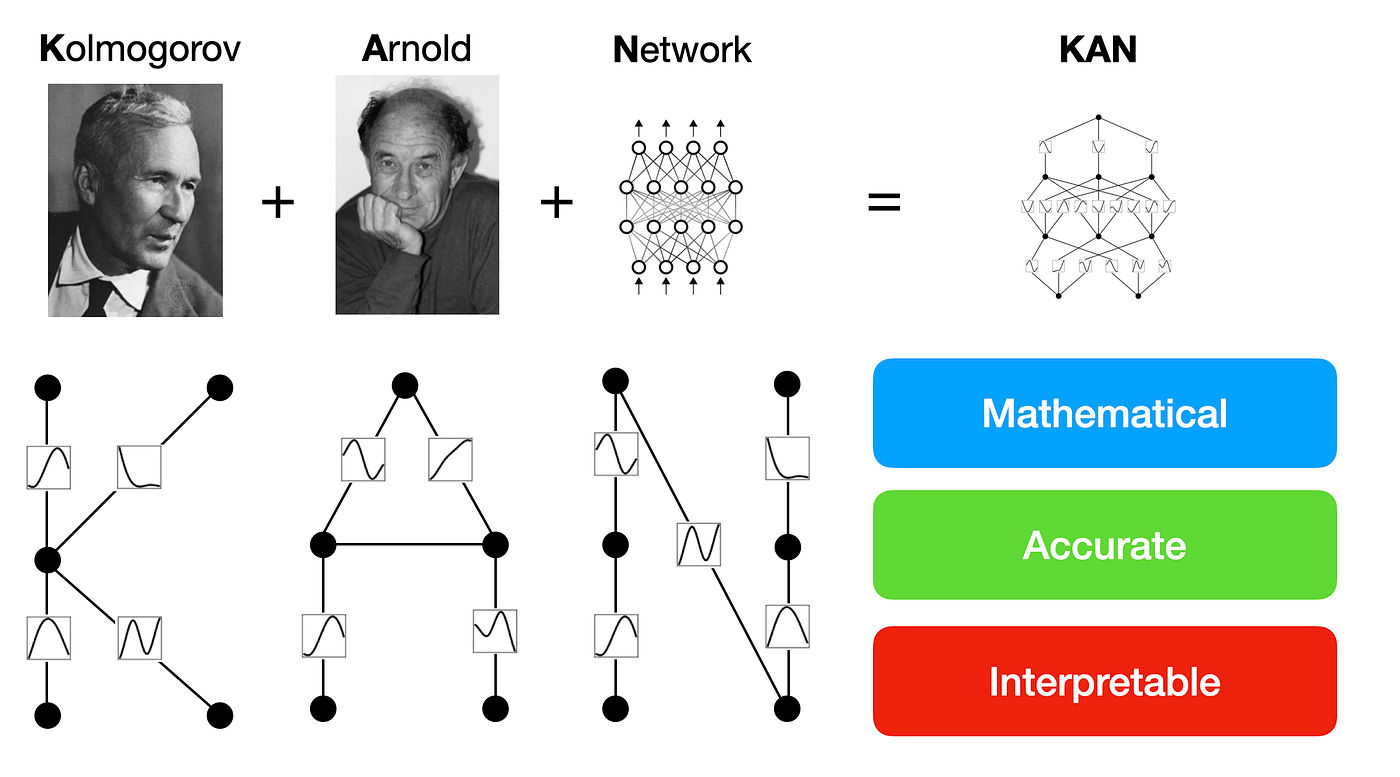
\includegraphics[width=1.0\textwidth]{img/kan_1st_image.png}
		\caption{Kolmogorov–Arnold Networks}
	\end{figure}
	
	\section{Fondamenti matematici}
	
	\subsection{Enunciato del teorema di Kolmogorov--Arnold}
	Il teorema di Kolmogorov–Arnold (KART) stabilisce che ogni funzione continua multivariata (cioè su più variabili), su un intervallo compatto, può essere espressa come una combinazione di somme di funzioni univariate (cioè su una variabile). In forma esplicita, per una funzione continua \(f:[0,1]^n \to \mathbb{R}\) esistono funzioni continue univariate \(\phi_{q,p}\) e \(\Phi_q\) tali che
	\[
	f(x_1,\dots,x_n)=\sum_{q=1}^{2n+1}\Phi_q\!\Biggl(\sum_{p=1}^n \phi_{q,p}(x_p)\Biggr),
	\]
	per \(q=1,\dots,2n+1\). \\
	Ciò signifca che ogni funzione continua multivariata può essere scomposta in una somma di funzioni univariate più semplici \(\Phi_q\), (dette funzioni esterne), ciascuna delle quali dipende da una combinazione lineare delle variabili originali trasformate tramite funzioni univariate, dette funzioni  interne \(\phi_{q,p}\). In questo contesto le funzioni interne agiscono da "features extractor", cioè estraggono informazioni rilevanti da ciascuna variabile, mentre le funzioni esterne combinano queste caratteristiche per produrre il valore finalle della funzione, agendo in modo simile ad un classificatore delle features estratte. Questo risultato afferma che qualsiasi funzione continua di più variabili può essere completamente rappresentata tramite combinazioni di funzioni continue di una sola variabile.
	
	\subsection{Sulla natura "non costruttiva" delle dimostrazioni}
	Le dimostrazioni originali del KART, eseguite da Kolmogorov nel 1957 e successivamente Arnold nel 1967, sono di natura esistenziale: garantiscono l'esistenza delle funzioni \(\phi_{q,p}\) e \(\Phi_q\), ma non forniscono una procedura esplicita o una formula chiusa per costruirle. Pertanto il teorema è fondamentale dal punto di vista teorico ma, senza ulteriori risultati costruttivi, ha un'utilità pratica limitata per la costruzione diretta di architetture neurali basate su tali funzioni, spingendo i ricercatori a privilegiare le reti neurali multistrato (MLP) che, pur con i loro limiti, erano più facili da implementare.
	
	\section{Architettura delle KAN}
	
	\begin{figure}[H]
		\centering
		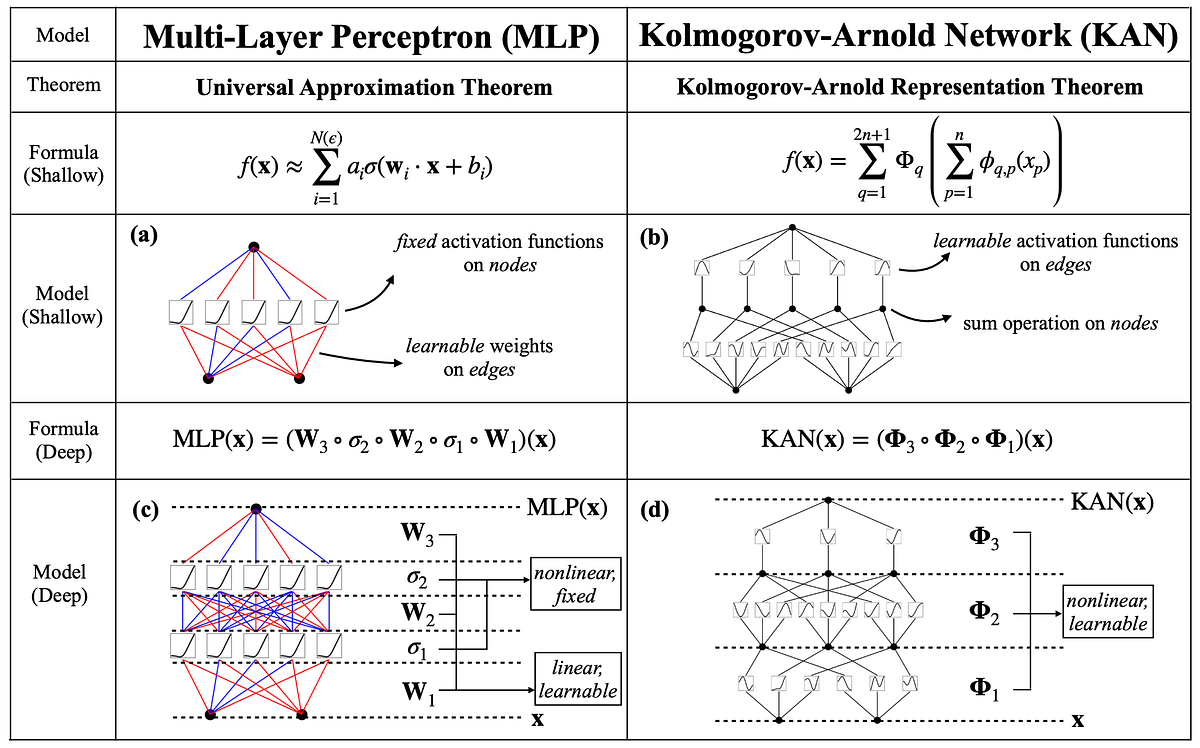
\includegraphics[width=1.0\textwidth]{img/KANvsMLP.png}
		\caption{Confronto tra Multi-Layer Perceptron (MLP) e Kolmogorov–Arnold Network (KAN).}
	\end{figure}
	Una KAN è strutturalmente simile ad una rete feedforward completamente connessa, simile ad una MLP, ma differisce in modo sostanziale nell'uso delle funzioni di attivazione: ogni arco (collegamento) tra i neuroni di strati consecutivi porta con sé una funzione univariata parametricamente definita (spesso una B-spline), anziché un peso scalare come nelle MLP. Ciascun neurone di uno strato riceve gli output dei collegamenti in ingresso e calcola semplicemente la somma di tali output, senza l’uso di pesi lineari o di funzioni di attivazione non lineari applicate ai singoli nodi stessi.
	
	Il modello generale si descrive così: se lo strato $(\ell-1)$ ha $d_{\ell-1}$ neuroni e lo strato $\ell$ ne ha $d_\ell$, allora esiste una matrice di funzioni unidimensionali $\{f^{(\ell)}_{ij}\}_{i=1,\dots,d_{\ell-1}}^{j=1,\dots,d_\ell}$ tale che, dati gli output degli $d_{\ell-1}$ neuroni precedenti $x_i^{(\ell-1)}$, l’uscita $x_j^{(\ell)}$ del $j$-esimo neurone del livello $\ell$ è: 
	\[
	x_j^{(\ell)} \;=\; \sum_{i=1}^{d_{\ell-1}} f^{(\ell)}_{ij}\bigl(x_i^{(\ell-1)}\bigr)\,.
	\] 
	In forma matriciale si può scrivere $x^{(\ell)} = f^{(\ell)}(x^{(\ell-1)})$, dove $f^{(\ell)}$ è l’insieme delle funzioni collegate a quello strato. L’output complessivo della KAN è quindi dato dalla composizione degli strati successivi: 
	\[
	y \;=\; x^{(L)} 
	= f^{(L)}\bigl(f^{(L-1)}(\dots f^{(1)}(x^{(0)})\dots)\bigr)\!,
	\] 
	dove $x^{(0)}$ è il vettore di input della rete. \\
	Questa architettura combina, in un’unica funzione $f_{ij}$ per ogni arco, le trasformazioni lineari e non lineari, permettendo alla rete di apprendere la forma esatta della funzione di attivazione necessaria per ogni arco di connessione. \\
	Si noti che un MLP applica funzioni di attivazione predefinite (ReLU, sigmoide, ecc.) sui singoli neuroni e moltiplica gli input per pesi scalari; al contrario, una KAN utilizza funzioni parametriche sugli archi e non applica ulteriori attivazioni non lineari sui neuroni.
	
	\subsection{Funzioni univariate parametriche}
	
	\begin{figure}[H]
		\centering
		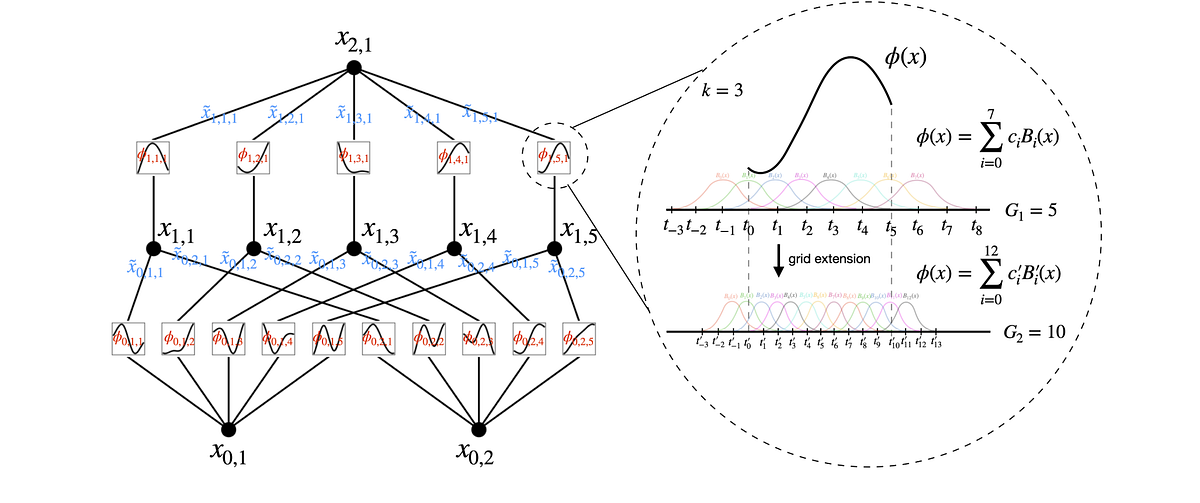
\includegraphics[width=1.0\textwidth]{img/fup.png}
		\caption{Struttura delle funzioni univariate parametriche.}
	\end{figure}
	
	Le funzioni di attivazione utilizzate nelle KAN sono funzioni univariate parametriche che possono apprendere flessibilmente la forma durante il training. Nell’implementazione classica proposta da Liu et al. (2024), queste funzioni sono rappresentate tramite B-spline (polinomi a tratti di basso grado), che offrono un buon trade-off tra flessibilità locale e complessità di calcolo. \\
	
	Ciascuna funzione di attivazione su un collegamento in una KAN è quindi espressa nella forma
	\[
	f_{ij}(t) = t + g_{ij}(t),
	\]
	dove \(g_{ij}(t)\) è una combinazione lineare di B-spline:
	\[
	g_{ij}(t) = \sum_{k=1}^{G+p} c_k B_{k,p}\left(\frac{t - t_{\min}}{t_{\max} - t_{\min}}\right).
	\]
	Il termine lineare \(t\) garantisce un comportamento affine iniziale, migliorando la stabilità dell'ottimizzazione durante il training, mentre il contributo spline introduce la non linearità appresa dalla rete, permettendo di modellare funzioni di attivazione flessibili e adattabili. \\
	Un aspetto importante è la definizione della spline grid, ovvero la suddivisione dell'asse degli input in nodi che delimitano gli intervalli su cui sono definiti i singoli segmenti delle B-spline. Il numero di nodi \(G\) e la loro posizione influenzano la capacità espressiva e la risoluzione locale delle funzioni attivazione. In generale, oltre alle B-spline, si possono utilizzare anche altre famiglie di funzioni unidimensionali parametriche, come i polinomi di Chebyshev o altre basi ortogonali, in base alle esigenze specifiche del problema. Infatti, le reti KAN sono in grado di adattare i coefficienti di queste basi durante il training, permettendo alla rete di apprendere funzioni di attivazione ottimali per ciascun collegamento.
	
	\subsection{B-spline}
	
	\begin{figure}[H]
		\centering
		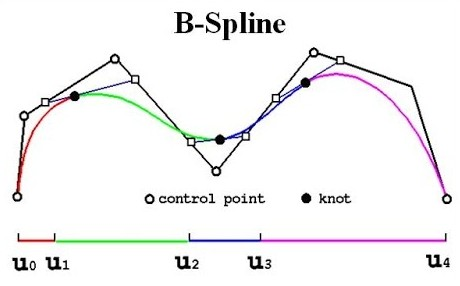
\includegraphics[width=1.0\textwidth]{img/b_spline.jpg}
		\caption{Struttura delle B-spline.}
	\end{figure}
	
	\subsubsection{Definizione}
	Le B-spline sono funzioni polinomiali a tratti che costituiscono la base per la rappresentazione di funzioni spline di un dato grado. Una B-spline di ordine \(p+1\) (ovvero di grado \(p\)) è definita ricorsivamente come segue:
	\[
	B_{i,0}(t) = \begin{cases}
		1 & \text{se } t_i \leq t < t_{i+1} \\
		0 & \text{altrimenti}
	\end{cases}
	\]
	e per \(p > 0\):
	\[
	B_{i,p}(t) = \frac{t - t_i}{t_{i+p} - t_i} B_{i,p-1}(t) + \frac{t_{i+p+1} - t}{t_{i+p+1} - t_{i+1}} B_{i+1,p-1}(t),
	\]
	dove \(\{t_i\}\) è il vettore dei nodi (knot vector), che suddivide il dominio della funzione in intervalli. Ogni B-spline \(B_{i,p}(t)\) è diversa da zero solo sull'intervallo \([t_i, t_{i+p+1})\), conferendo proprietà di supporto locale.
	
	\subsubsection{Implementazione delle B-spline nelle KAN}
	
	Nelle implementazioni standard delle KAN, le funzioni di attivazione sui collegamenti sono parametrizzate come combinazioni lineari di B-spline cubiche (\(p=3\)):
	\[
	f_{ij}(x) = w_0 x + \sum_{k=1}^{G+p} c_k B_{k,p}\left(\frac{x - x_{\min}}{x_{\max} - x_{\min}}\right),
	\]
	dove:
	\begin{itemize}
		\item \(w_0\) è il termine residuo lineare che garantisce un comportamento iniziale affine,
		\item \(\{c_k\}\) sono i coefficienti addestrabili della spline,
		\item \(G\) è il numero di intervalli della griglia di nodi,
		\item \(B_{k,p}\) sono le funzioni base B-spline di grado \(p\).
	\end{itemize}
	Il termine residuo lineare \(w_0 x\) stabilizza l’ottimizzazione, permettendo alla funzione di partire come lineare e apprendere non linearità tramite la componente spline.
	
	\subsubsection{Adattamento della griglia}
	Un aspetto importante delle KAN è l’adattamento dinamico della spline grid. Inizialmente, la griglia è generalmente uniforme, ma può essere ampliata aumentando il numero di nodi. Durante il training, i nodi possono essere riposizionati strategicamente per concentrare la risoluzione nelle aree in cui la funzione varia maggiormente, migliorando così la capacità di modellazione locale della rete. Per mantenere la stabilità durante queste modifiche alla griglia, si utilizzano tecniche di interpolazione lineare sui parametri dell’ottimizzatore, garantendo transizioni fluide e controllate nella definizione della griglia.
	
	\subsection{Scaling laws e Curse of dimensionality}
	Come suggerito dal teorema matematico KART, le KAN godono di proprietà di approssimazione analoghe ma più raffinate rispetto alle MLP. In particolare, il teorema di Kolmogorov-Arnold garantisce che ogni funzione continua multivariata definita su un dominio compatto possa essere rappresentata esattamente come composizione di funzioni univariate e somme, realizzabile da una KAN con 2 strati e larghezza proporzionale all'input $n$ (in particolare, larghezza $2n + 1$).
	Di conseguenza, per ogni tolleranza $\epsilon > 0$ esiste una KAN sufficientemente ampia che approssima la funzione $f$ entro errore $\epsilon$, cioè
	\begin{equation*}
		\| f_{\mathrm{KAN}} - f \| < \epsilon.
	\end{equation*}
	Questa capacità permette alle KAN di superare il problema noto come curse of dimensionality, a condizione che la funzione da approssimare possieda una struttura additivo-composizionale sufficientemente regolare. In particolare, l'errore di approssimazione di una KAN dipende principalmente dalla risoluzione della griglia spline utilizzata nelle funzioni univariate, risultando approssimativamente indipendente dalla dimensione dell'input. Questa proprietà si traduce in scaling laws più favorevoli rispetto alle MLP tradizionali, per le quali il numero di parametri necessari per garantire una certa accuratezza generalmente cresce esponenzialmente con la dimensione dell'input. Il vantaggio teorico delle KAN deriva dal fatto che esse, a differenza delle MLP, apprendono non solo la struttura composizionale della funzione, ma sono anche in grado di modellare con elevata precisione le funzioni univariate interne, grazie all’uso di attivazioni parametriche basate su spline.
	
	\section{Funzionamento operativo}
	
	\subsection{Calcolo del mapping input–hidden–output}
	
	Nel funzionamento operativo di una KAN, i dati scorrono in avanti attraverso gli strati esattamente come in una normale MLP, ma usando le funzioni di attivazione sugli archi. Dato un vettore di input $x^{(0)}$, il calcolo procede layer dopo layer: per ciascun neurone nel primo strato nascosto si valuta la somma delle funzioni dei collegamenti in ingresso applicate alle componenti di $x^{(0)}$, ottenendo $x^{(1)}$ e così via. Al livello successivo si ripete lo stesso procedimento prendendo $x^{(1)}$ come input, e così via fino allo strato di output. Formalmente, ogni layer $\ell$ esegue la trasformazione $x^{(\ell)} = f^{(\ell)}(x^{(\ell-1)})$, e l’output finale è $y = x^{(L)}$. \\
	Poiché tutte le operazioni, cioè l’applicazione delle funzioni univariate e le somme, sono differenziabili, l'intero modello è addestrabile tramite backpropagation. Questo significa che i coefficienti delle funzioni di attivazione (ad esempio, delle spline) possono essere ottimizzati tramite discesa del gradiente, minimizzando una funzione di perdita, allo stesso modo di quanto avviene in un MLP.
	
	\subsection{Processo di training e Calcolo dei pesi}
	
	Il training di una KAN segue la procedura standard di addestramento supervisionato con discesa del gradiente. Si parte da un dataset di training ed una funzione loss, quindi si aggiornano iterativamente i parametri delle funzioni di attivazione. Nelle KAN, i "pesi" da addestrare sono i coefficienti che definiscono le funzioni unidimensionali sui collegamenti. Per esempio, una spline di ordine 3 su $r$ intervalli ha $r+3$ coefficienti; ciascun coefficiente è un parametro della rete. È comune includere un termine base lineare (di solito la stessa identità), come in 
	\[
	f_{ij}(t) = t + g_{ij}(t)\,, 
	\]
	dove $g_{ij}$ è la spline addestrabile. Questo facilita la convergenza iniziale. \\
	Durante l’ottimizzazione si può anche aggiornare adattivamente la griglia di definizione delle spline, così da coprire automaticamente i nuovi intervalli di attivazione che emergono durante il training (grid extension). In pratica, ogni volta che un valore di attivazione supera la griglia corrente, si estende dinamicamente il supporto della spline per mantenere il dominio di apprendimento adeguato. In sintesi, il flusso di calcolo è identico ad un MLP: si effettua forward pass, si calcola la loss, e poi si retropropaga l’errore calcolando gradienti rispetto ai coefficienti delle funzioni $g_{ij}$.
	
	\section{Confronto con MLP tradizionali}
	
	\begin{figure}[H]
		\centering
		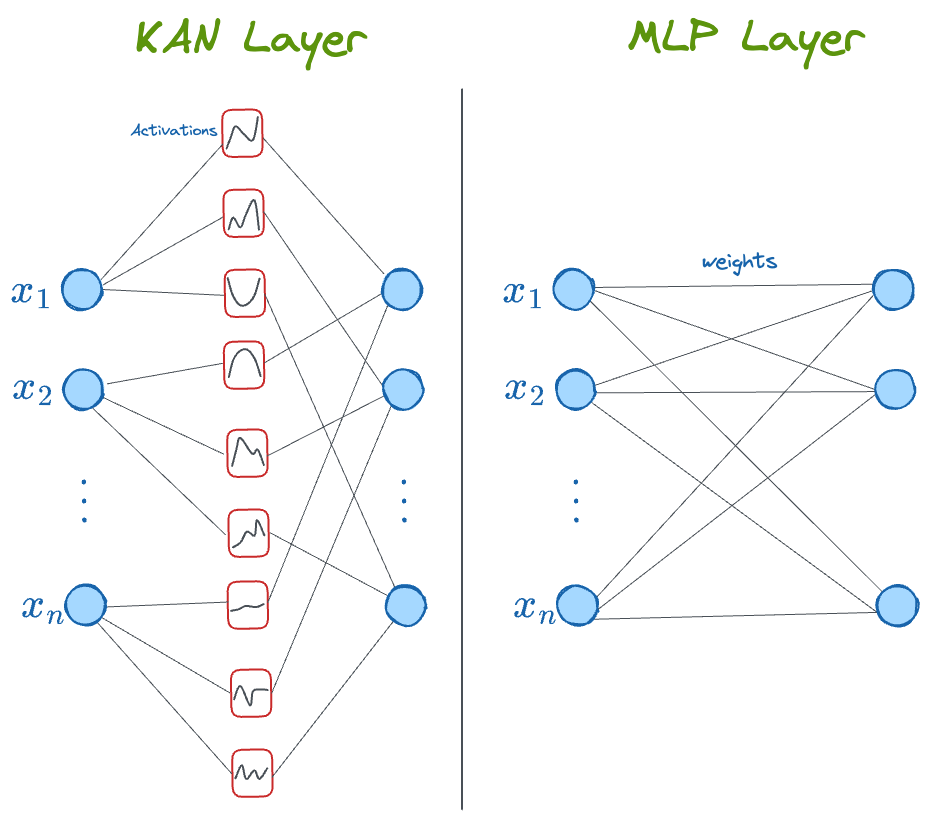
\includegraphics[width=1.0\textwidth]{img/KANvsMLP_layer.png}
		\caption{Differenze tra i Layer delle reti MLP e KAN.}
	\end{figure}
	
	\subsection{Architettura a confronto}
	Dal punto di vista architetturale, l’architettura di base di una KAN è feedforward e totalmente connessa come quella di un MLP. La differenza fondamentale risiede nel collocamento delle non-linearità e nell’assenza di matrici di pesi lineari. Come abbiamo visto, in un MLP ogni neurone applica una funzione di attivazione fissa, dopo una combinazione lineare dei suoi input, mentre in una KAN ogni collegamento possiede direttamente una funzione di attivazione addestrabile. Di conseguenza, una KAN "unisce" le trasformazioni lineari e non-lineari in un’unica funzione $f_{ij}$ per ogni arco, anziché trattarle separatamente come in un MLP. \\
	In termini pratici, una MLP a $L$ strati alterna operazioni $x \mapsto W x + b$ e $x \mapsto \sigma(x)$, mentre una KAN sostituisce ogni prodotto $W_{ij}x_i$ con $f_{ij}(x_i)$. Questo implica che una KAN può essere vista come un MLP "con pesi che variano in modo non-lineare col valore dell'input". \\
	
	\subsection{Complessità computazionale}
	Dal punto di vista parametrico, una KAN può avere un numero di parametri superiore rispetto ad una MLP di dimensioni simili. Ad esempio, supponiamo una KAN con $L$ strati, ciascuno di larghezza $m$, che usa spline di ordine $p$ su $r$ intervalli. Allora il numero totale dei parametri della rete KAN cresce come $\mathcal{O}(L\,m^2\,p\,r)$, mentre una MLP con $L$ strati e larghezza $m$ avrebbe circa $\mathcal{O}(L\,m^2)$ pesi scalari. In teoria quindi le KAN appaiono meno efficienti in termini di numero di parametri. Tuttavia, empiricamente si osserva che spesso basta una KAN con dimensioni molto più piccole per eguagliare le prestazioni di una MLP molto più grande. Dal punto di vista computazionale, l’impiego di funzioni parametriche sugli archi comporta un overhead rispetto alle semplici moltiplicazioni peso-input di una MLP. In pratica, valutare una B-spline su ogni collegamento è più costoso del prodotto scalare in una MLP, soprattutto se la rete è profonda o le spline sono molto finemente discretizzate (cioé utilizzano un numero elevato di punti di controllo). Quindi, l'addestramento di una KAN, può essere più lento, con stime che indicano un tempo di training circa 10 volte superiore rispetto alle MLP a parità di condizioni.
	
	\subsection{Interpretabilità e flessibilità locale}
	Uno dei principali vantaggi delle KAN è la loro interpretabilità. Poiché ogni arco implementa una funzione univariata ben definita, è possibile visualizzare direttamente le forme delle attivazioni apprese. Questo permette di comprendere i singoli contributi delle variabili di input e, in alcuni casi, di dedurre formule simboliche sottostanti, oltre a rendere più semplice il debug e la semplificazione del modello. \\
	\begin{figure}[H]
		\centering
		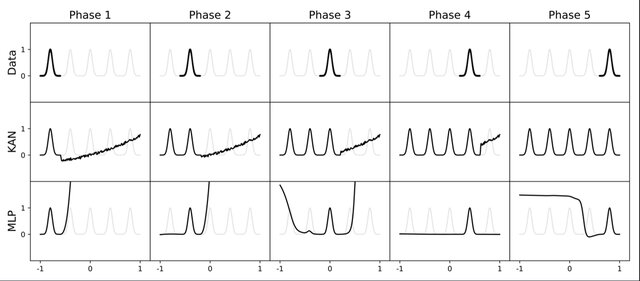
\includegraphics[width=1.0\textwidth]{img/Catastrophic_forgetting_KANvsMLP.jpg}
		\caption{Differenza nel Catastrophic forgetting di MLP e KAN.}
	\end{figure}
	Un altro vantaggio importante è la flessibilità locale che deriva dalla natura delle spline. A differenza delle MLP che usano funzioni di attivazione globali (come ReLU o Tanh), una KAN modifica solo una piccola regione di input quando apprende una nuova informazione. Ciò riduce significativamente il rischio di "catastrophic forgetting", un fenomeno in cui l'addestramento su nuovi dati può distruggere le informazioni precedentemente apprese.
	
	\subsection{Precisione controllabile tramite grid extension}
	\begin{figure}[H]
		\centering
		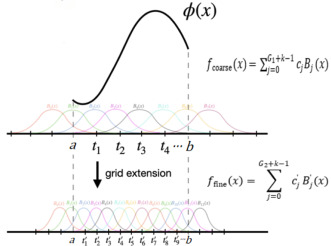
\includegraphics[width=0.7\textwidth]{img/grid_extension.jpg}
		\caption{Grid extension delle B-spline nelle KAN.}
	\end{figure}
	Le funzioni univariate nelle KAN sono parametrizzate tramite B-spline definite su una griglia. È possibile aumentare la risoluzione della griglia ("grid extension") per incrementare la precisione in modo controllato: partendo da spline grossolane si possono ottenere spline più fini con una procedura di inizializzazione che conserva la continuità e permette rapide riduzioni della loss senza costi computazionali esponenziali.
	
	\subsection{Dipendenza dalla struttura composizionale}
	I vantaggi più evidenti delle KAN si manifestano quando la funzione target da approssimare ha una struttura che si avvicina ad una decomposizione in somme di funzioni univariate, cioè può essere sufficientemente rappresentata come somma di trasformazioni su singole variabili. Quando la funzione è intrinsecamente non decomponibile o presenta forti interazioni multivariate, la rappresentazione KAN perde efficacia e può risultare meno efficiente rispetto ad una parametrizzazione densa tipica delle MLP.
	
	\subsection{Irregolarità nella rappresentazione di Kolmogorov}
	Il teorema di Kolmogorov–Arnold garantisce l'esistenza di una rappresentazione, ma non la regolarità delle funzioni intermedie \(\varphi_{q,p}\). In casi pratici, queste funzioni possono essere non-smooth o altamente oscillanti; per approssimarle con spline possono essere necessarie griglie molto fitte, annullando i vantaggi teorici in termini di parametri e costo computazionale.
	
	\subsection{Overhead computazionale e scelta della struttura}
	Parametrizzare ogni arco come funzione spline introduce overhead in memoria ed in tempo di calcolo (valutazione e aggiornamento di B-spline, gestione di griglie differenziate). Inoltre, la scelta automatica della topologia (numero di rami, profondità, risoluzione delle griglie per ciascuna spline) non è banale e richiede procedure di pruning o ricerca strutturale che aumentano la complessità del workflow.
	
	\subsection{Sensibilità al rumore e necessità di regolarizzazione}
	In presenza di dati molto rumorosi, una parametrizzazione spline troppo fine tende al sovraffitting locale. È quindi necessario un attento tuning degli iperparametri (ordine della spline, numero di nodi, termine di regolarizzazione, smoothing), e in alcuni casi una MLP ben regolarizzata può mostrare maggiore robustezza.
	
	\chapter{Random forest}
	
	\section{Introduzione}
	In questo capitolo viene descritto il Random forest, un algoritmo di Machine learning molto versatile, in grado di gestire sia compiti di classificazione che di regressione. Il suo funzionamento si basa sull'idea dell'ensemble learning, combinando la forza di più alberi di decisione per ottenere un modello finale più robusto e preciso. L'introduzione del capitolo si concentra sui concetti fondamentali che guidano la costruzione del modello, come i criteri di divisione dei dati e la tecnica di bagging, che sfrutta il campionamento casuale per ridurre la varianza. Si approfondisce poi l'architettura specifica del Random forest, che aggiunge un ulteriore livello di casualità nella selezione delle variabili per ogni albero, rendendo la "foresta" più diversificata e meno soggetta ad overfitting. Il capitolo si conclude con una valutazione dei vantaggi e degli svantaggi dell'algoritmo, evidenziando la sua robustezza e la sua capacità di generalizzazione, ma anche i suoi requisiti in termini di risorse computazionali e la minore interpretabilità rispetto ad un singolo albero. \cite{breiman2001randomforest, quinlan1993c45, breiman1996bagging, fatima2023xgbvsrf}
	
	\begin{figure}[H]
		\centering
		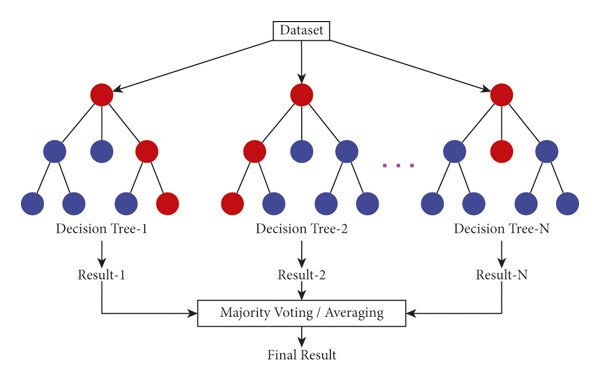
\includegraphics[width=0.8\textwidth]{img/rf.png}
		\caption{Architettura del Random forest.}
	\end{figure}
	
	Il Random forest è un algoritmo di Machine learning ampiamente utilizzato, noto per la sua robustezza e versatilità sia in problemi di classificazione e regressione. La sua efficacia deriva dalla combinazione di più alberi di decisione "deboli", formando un "ensemble" che supera le prestazioni di un singolo albero, mitigando le debolezze di ciascuno.
	
	\section{Concetti fondamentali}
	
	\subsection{Alberi di decisione: Criteri di splitting (Gini, Entropia, Gain ratio)}
	
	Gli alberi di decisione costituiscono i "learner deboli" fondamentali all'interno di un Random forest. La loro costruzione implica la divisione iterativa dei dati basata sulle features per creare sottoinsiemi sempre più omogenei. La qualità di queste divisioni è misurata da specifici criteri di impurità o Information gain. Il Gini impurity (o Gini index) è una misura di non-omogeneità ampiamente utilizzata negli alberi di classificazione. Essa quantifica la probabilità che un elemento scelto casualmente da un set venga erroneamente etichettato, se classificato in modo casuale, secondo la distribuzione delle classi nel sottoinsieme. Un valore di 0 indica purezza perfetta, dove tutti gli elementi appartengono alla stessa classe, mentre un valore massimo di $1 - \frac{1}{n}$, dove $n$ é il numero di classi, indica la massima impurità, con le classi equamente distribuite. La formula per il Gini impurity è data da:
	
	$$Gini = 1 - \sum_{i=1}^{n} (p_i)^2$$
	
	dove $p_i$ rappresenta la proporzione delle istanze della classe $i$ nel set. Ad esempio, se un nodo contiene 50 campioni, di cui 25 di una classe e 25 di un'altra, l'impurità di Gini sarebbe 0.5, indicando la massima incertezza. Dopo uno split, l'algoritmo seleziona la variabile che produce la maggiore diminuzione dell'impurità di Gini, portando a nodi più puri. \\
	L'Entropia (Entropy) misura il grado di disordine, imprevedibilità o incertezza in un dataset. Un'entropia di 0 indica un set perfettamente puro, mentre un valore di $\log_2(n)$ indica la massima incertezza. L'Information gain misura la riduzione dell'entropia ottenuta da uno split, indicando quanta "informazione" viene acquisita sulla variabile target. La formula per l'Entropia è:
	
	$$Entropy = - \sum_{i=1}^{n} p_i \log_2(p_i)$$
	
	dove $p_i$ è la probabilità della classe $i$. \\
	Il Gain ratio è stato introdotto per mitigare un problema dell'Information gain, che ha un bias verso attributi con un gran numero di valori. Questi attributi tendono a creare molti nodi piccoli e puri, il che può condurre a un potenziale overfitting. Il Gain ratio normalizza l'Information gain, penalizzando gli split che creano molti sottoinsiemi. La sua formula è:
	
	$$Gain ratio = \frac{Information gain}{Split information}$$
	
	dove lo $Split$ $information$ è l'entropia dello split stesso:
	
	$$Split Information(S, A) = - \sum_{i=1}^{v} \frac{|S_i|}{|S|} \log_2(\frac{|S_i|}{|S|})$$
	
	dove $S$ è il set di dati del nodo, $A$ è la feature su cui si sta splittando, $v$ è il numero di valori unici della feature, $|S_i|$ è il numero di istanze nel sottoinsieme $i$ e $|S|$ è il numero totale di istanze. \\
	Un confronto tra Gini impurity, Entropia e Gain ratio rivela differenze importanti. Il Gini impurity ha un intervallo di valori compreso tra $[0, 1 - \frac{1}{n}]$, mentre l'Entropia ha un intervallo tra $[0, \log_2(n)]$. Dal punto di vista computazionale, il Gini index è generalmente più efficiente da calcolare rispetto all'Entropia, poiché quest'ultima richiede l'uso di logaritmi. La scelta tra i criteri non è arbitraria, ma implica un compromesso. Il Gini, essendo computazionalmente più veloce, è meno incline a produrre alberi di decisione molto profondi, poiché privilegia split che generano nodi più bilanciati. Al contrario, l'Entropia, sebbene più onerosa, tende a generare alberi che massimizzano la riduzione dell'incertezza, ma il suo bias può portare a preferire caratteristiche con molte categorie, aumentando il rischio di overfitting. Per mitigare ciò, il Gain Ratio si dimostra più robusto. \\
	Per dataset molto grandi o per applicazioni con stringenti requisiti di velocità, il Gini potrebbe essere la scelta preferibile. Per contro, in contesti dove la massima purezza dei nodi è cruciale, l'Entropia (o, più precisamente, il Gain ratio) potrebbe rivelarsi più efficace, a condizione che il rischio di overfitting venga gestito adeguatamente. Questa decisione fondamentale, a livello del singolo albero, si ripercuote sulla performance e sulla struttura complessiva del Random forest. Un albero "più debole" ma più rapido, generato con il Gini, può essere efficacemente compensato dall'approccio Ensemble, mentre alberi "più forti" ma più lenti, derivanti dall'Entropia, potrebbero non scalare con la stessa efficienza.
	
	\subsection{Ensemble learning e Bagging}
	
	Il principio alla base dell'Ensemble learning è spesso descritto come la "saggezza della folla": un gruppo di learner deboli, che individualmente potrebbero non performare in modo ottimale, a causa di alta varianza o alto bias, può, quando le loro previsioni vengono aggregate, formare un "learner forte" con prestazioni notevolmente migliorate. \\
	\begin{figure}[H]
		\centering
		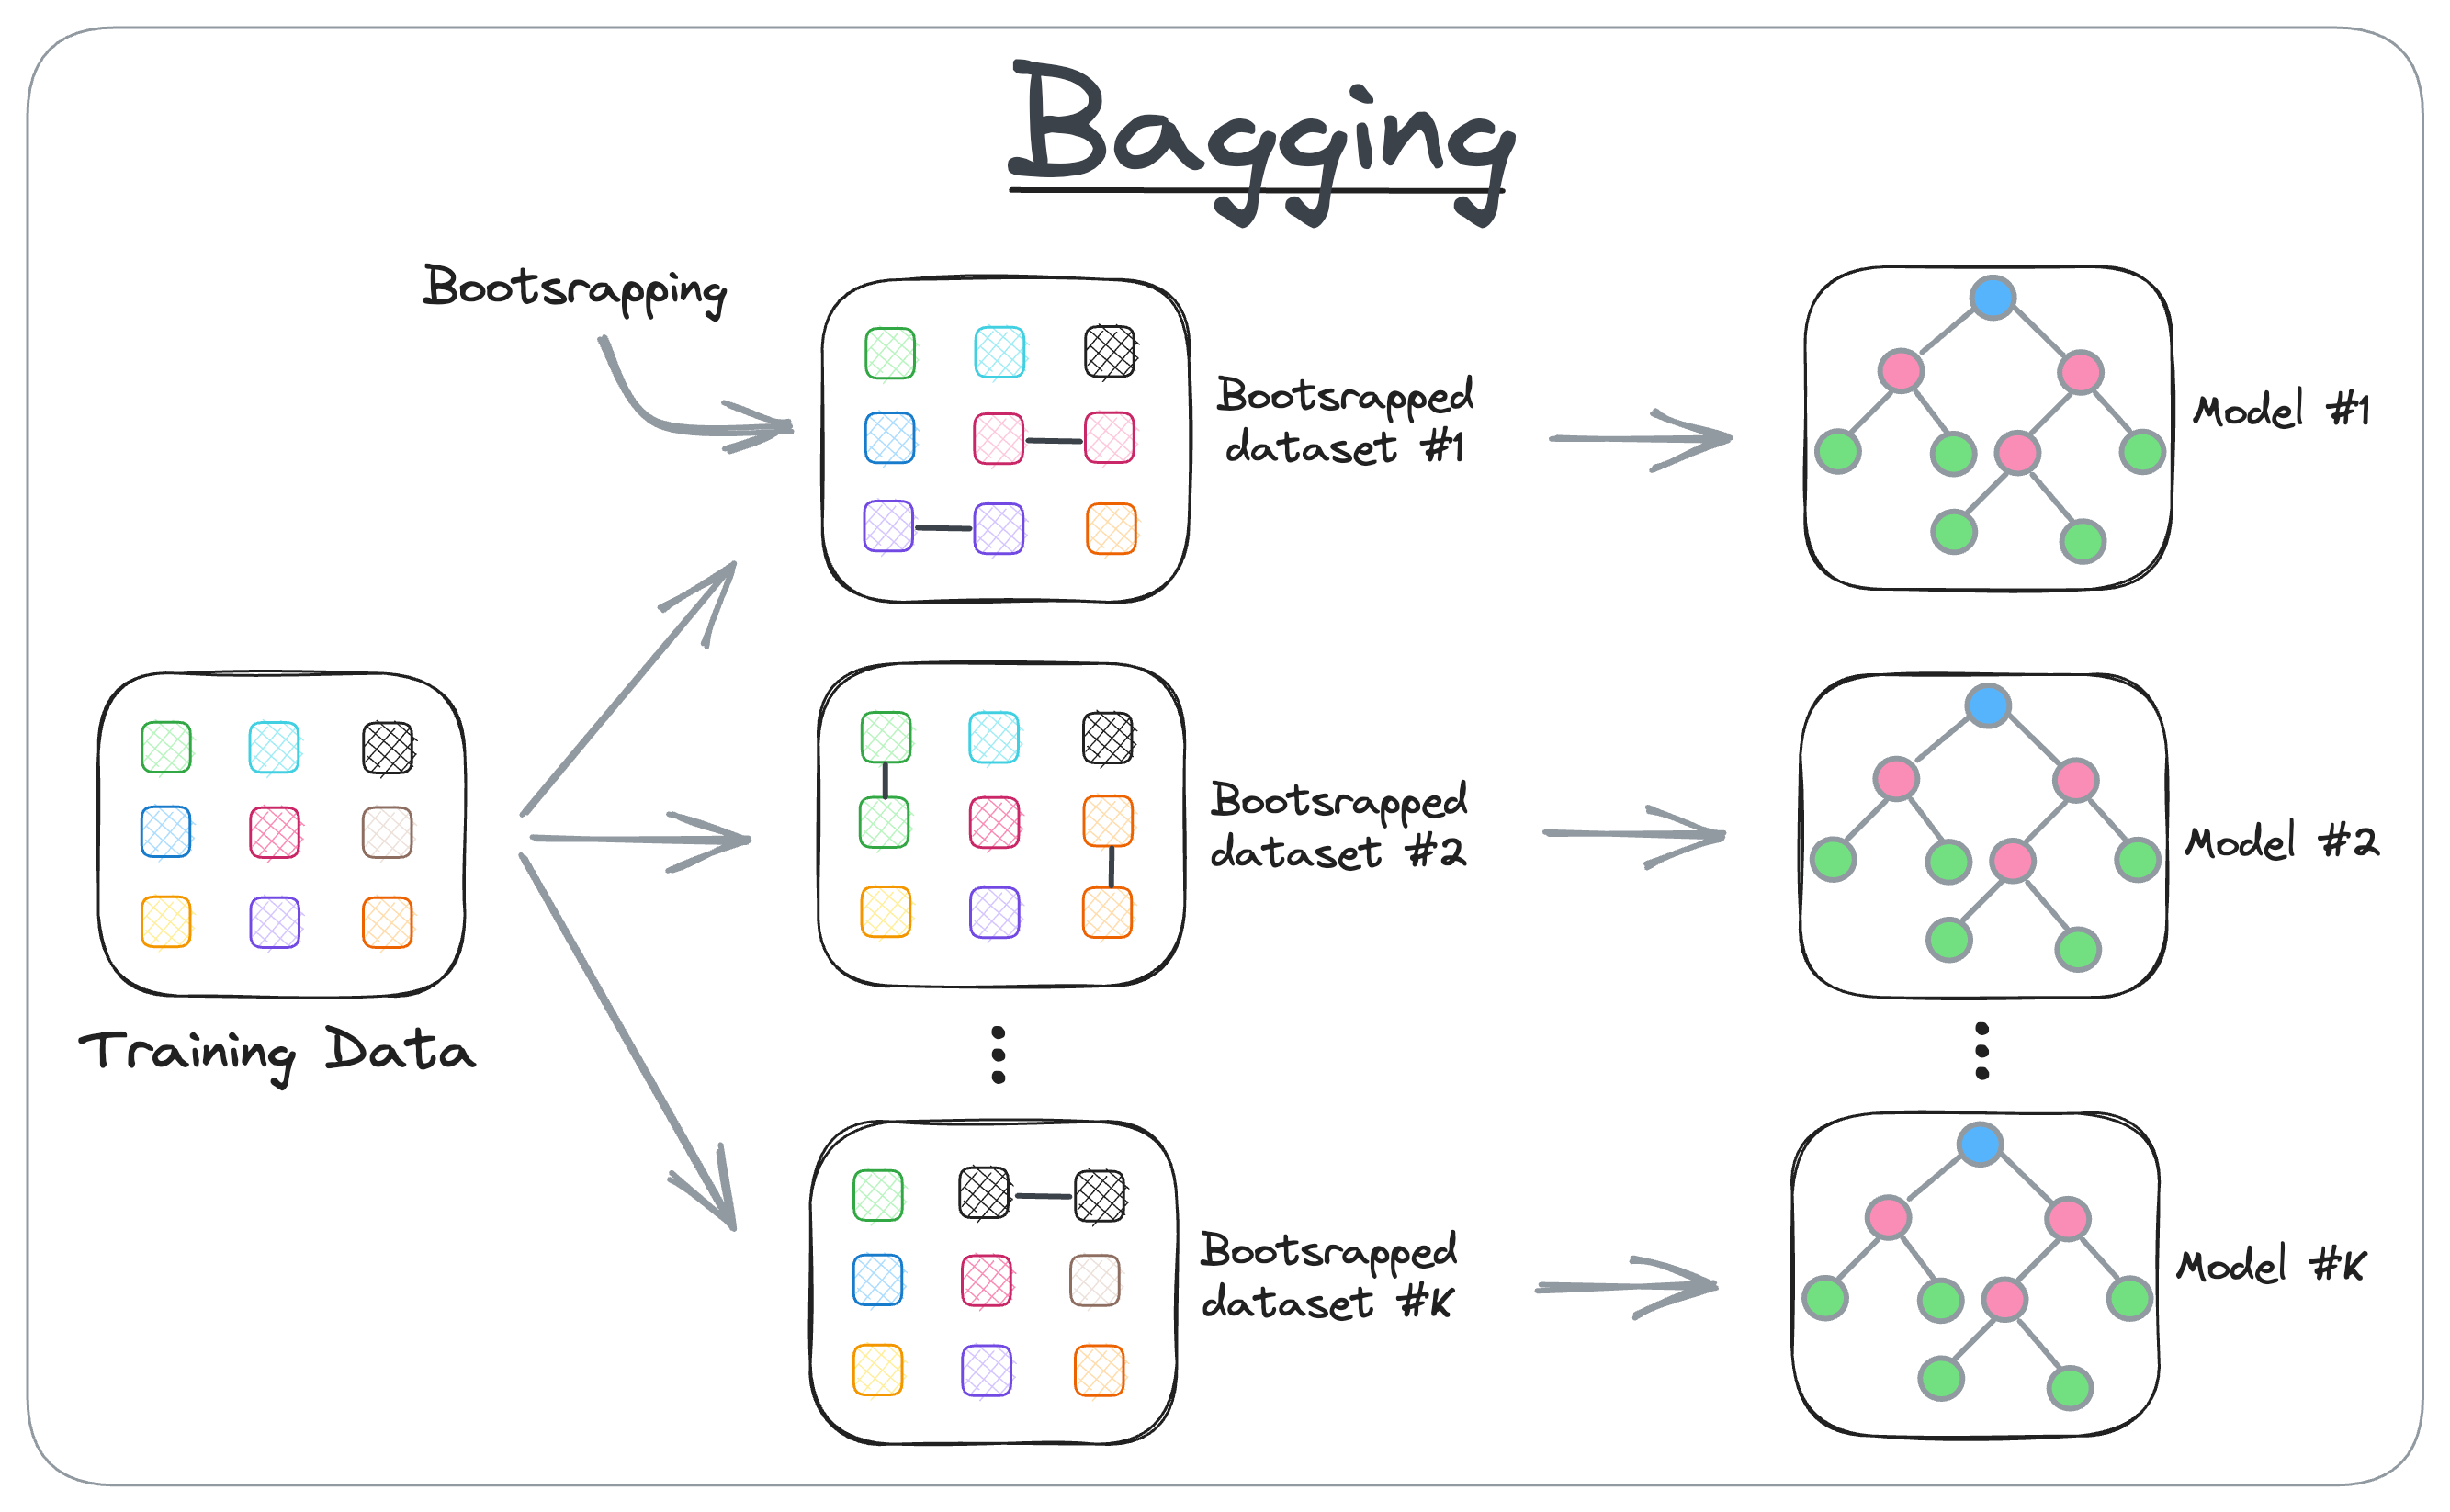
\includegraphics[width=0.8\textwidth]{img/bagging.png}
		\caption{Funzionamento del Bagging.}
	\end{figure}
	Il Bagging è un metodo di Ensemble learning il cui scopo principale è ridurre la varianza all'interno di un dataset "rumoroso", migliorando così la capacità di generalizzazione del modello e mitigando l'overfitting. Il processo di Bagging si articola in tre fasi fondamentali:
	\begin{enumerate}
		\item \textbf{Bootstrapping}: questa tecnica di ricampionamento genera diversi sottoinsiemi del training set. Il campionamento avviene selezionando istanze in modo casuale con re-immissione, ciò significa che una singola istanza può essere scelta più volte all'interno dello stesso sottoinsieme. Questo processo è cruciale per creare diversità tra i campioni su cui verranno addestrati i modelli individuali.
		\item \textbf{Addestramento parallelo}: i campioni bootstrap così generati vengono utilizzati per addestrare, in modo indipendente e parallelo, una serie di learner deboli, che nel contesto di Random forest sono tipicamente alberi di decisione.
		\item \textbf{Aggregazione}: una volta che i modelli individuali hanno prodotto le loro previsioni, queste vengono combinate. Per i problemi di regressione, si utilizza un processo noto come Soft voting (cioè la media di tutti gli output previsti dai singoli learner), mentre, per i problemi di classificazione, si utilizza l'Hard o Majority voting (cioè viene scelta la classe più votata).
	\end{enumerate}
	
	Il beneficio più significativo è la riduzione della varianza, particolarmente utile con dati ad alta dimensionalità o in presenza di valori mancanti, dove un'alta varianza può rendere il modello più incline all'overfitting. La diversità introdotta nei dati di training per ciascun modello contribuisce a ridurre la varianza nelle previsioni finali. Questo processo mitiga l'influenza del rumore nei dati e degli outlier, producendo un modello aggregato più stabile ed affidabile. Tuttavia, il Bagging può portare ad una perdita di interpretabilità, rendendo difficile estrarre intuizioni precise a causa del processo di media delle previsioni. È anche computazionalmente costoso, rallentando e diventando più intensivo all'aumentare del numero di iterazioni. Infine, è meno flessibile con algoritmi già stabili o con un alto bias, poiché i benefici, in termini di riduzione della varianza, sono meno visibili. \\
	Il Bagging non è semplicemente un metodo per combinare modelli, ma agisce come una forma intrinseca di regolarizzazione. Addestrando modelli su sottoinsiemi diversi del dataset, ottenuti attraverso il campionamento di tipo bootstrap, ciascun modello apprende una prospettiva leggermente differente del problema. Quando le previsioni di questi modelli, sebbene diversi, sono aggregate, gli errori casuali e la varianza intrinseca di un singolo modello tendono a compensarsi reciprocamente. Ciò porta a una previsione finale che è più stabile e meno sensibile al rumore oppure agli outlier. Questo meccanismo è la ragione fondamentale per cui il Bagging è così efficace nel ridurre l'overfitting, specialmente per learner ad alta varianza, come gli alberi di decisione profondi. Questa capacità di ridurre la varianza senza introdurre un bias significativo rende il Bagging una base così potente per algoritmi come Random forest, che altrimenti sarebbero molto inclini all'overfitting. È una dimostrazione del principio che la "diversità" all'interno di un ensemble conduce a una maggiore robustezza del modello complessivo.
	
	\section{Architettura e Costruzione}
	
	Random forest estende il concetto di Bagging introducendo un ulteriore livello di casualità, rendendo l'Ensemble ancora più robusto e meno propenso all'overfitting.
	
	\subsection{Bootstrapping e Feature bagging}
	
	La costruzione di un Random forest si basa su due fonti principali di casualità, essenziali per garantire che gli alberi individuali siano il più possibile non correlati tra loro. \\
	La prima fonte di casualità è il campionamento di tipo bootstrap. Per ogni albero che fa parte della foresta, viene estratto un campione casuale di dati dal set di training originale con re-immissione. Questo sottoinsieme di dati è noto come Bootstrap sample. Una caratteristica importante di questo processo è che circa un terzo dei dati originali non viene selezionato per un dato bootstrap sample; questi dati non utilizzati sono chiamati campioni "out-of-bag" e possono essere impiegati per la validazione interna del modello. Questo tipo di campionamento assicura che ogni albero sia addestrato su un sottoinsieme leggermente diverso dei dati originali, promuovendo una diversità fondamentale tra gli alberi. \\
	La seconda fonte di casualità è legata alle features, nota come feature bagging o random subspace method. Ad ogni split dei nodi, all'interno di un albero di decisione, Random forest non considera tutte le feature disponibili, ma seleziona solo un sottoinsieme casuale di esse. Questa è una differenza importante rispetto agli alberi di decisione standard, che valuterebbero tutte le feature possibili per trovare lo split migliore. L'introduzione di questa casualità nella selezione delle feature aggiunge ulteriore diversità al dataset per ogni albero e riduce significativamente la correlazione tra gli alberi di decisione individuali. \\
	La casualità introdotta nel Random Forest, tramite bootstrapping e feature bagging, non è ridondante, ma complementare e strategica. Il Bootstrapping riduce la varianza generale del modello assicurando che ogni albero acquisisca una prospettiva leggermente diversa del dataset complessivo. Il Feature bagging, d'altra parte, previene che caratteristiche particolarmente forti o dominanti influenzino la costruzione di tutti gli alberi. Se una singola caratteristica fosse sempre scelta come il miglior punto di split, tutti gli alberi all'interno della foresta risulterebbero molto simili e altamente correlati, rendendo inutili i benefici derivanti dall'approccio Ensemble. Introducendo la casualità nella selezione delle feature, si forza ogni albero ad esplorare diverse combinazioni di caratteristiche, riducendo ulteriormente la loro correlazione e, di conseguenza, la varianza dell'intero Ensemble.
	
	\subsection{Aggregazione delle predizioni}
	
	Una volta che tutti gli alberi di decisione sono stati costruiti e addestrati sui rispettivi sottoinsiemi di dati e feature, le loro previsioni vengono combinate per ottenere il risultato finale del Random forest. Il metodo di aggregazione dipende dalla natura del problema. Nei problemi di regressione, le previsioni numeriche generate da ciascun albero individuale vengono semplicemente mediate. Il valore medio di tutte le previsioni degli alberi costituisce la previsione finale del modello. Nei problemi di classificazione, la classe finale viene determinata attraverso un processo di voto di maggioranza. Ogni albero nella foresta produce una previsione e la classe che riceve il maggior numero di "voti" (cioè, la più scelta) tra tutti gli alberi viene accettata come previsione finale del Random forest. \\
	Questo processo di aggregazione trasforma un insieme di learner deboli in un modello forte. Sebbene gli alberi di decisione individuali possano presentare un'alta varianza, la media o il voto di maggioranza sulle loro previsioni riduce significativamente la varianza complessiva e rende il modello meno sensibile ad errori ed outlier. Questo processo mitiga la tendenza del singolo albero a sovrastimare o sottostimare i valori, producendo una previsione finale più stabile e robusta. Questo meccanismo di aggregazione è ciò che consente al Random forest di raggiungere un'elevata accuratezza mantenendo al contempo una solida capacità di generalizzazione. È un esempio pratico dell'applicazione del principio della "saggezza della folla" nel Machine learning, dove la combinazione di molteplici opinioni individuali, seppur imperfette, conduce ad un risultato finale superiore.
	
	\section{Vantaggi}
	Il Random Forest si distingue per la sua robustezza e flessibilità, offrendo diversi vantaggi che lo rendono una scelta popolare nel machine learning. Un punto di forza principale è la \textbf{riduzione della varianza}, che lo rende intrinsecamente meno propenso all'overfitting rispetto a un singolo albero di decisione. Questo risultato è ottenuto grazie alla sua natura ensemble, che aggrega le previsioni di molti alberi indipendenti, ed all'introduzione di casualità sia nel campionamento dei dati (bootstrap) sia nella selezione delle feature per ogni singolo albero. La sua robustezza non si limita alla varianza. L'algoritmo mostra anche una notevole \textbf{robustezza agli outlier}, poiché l'impatto di singole osservazioni estreme viene diluito e mediato tra i vari alberi. Il Random Forest eccelle anche nella \textbf{gestione dei valori mancanti}, semplificando notevolmente la fase di pre-elaborazione dei dati. Allo stesso modo, è in grado di gestire efficacemente \textbf{dataset sbilanciati}. Dal punto di vista della usabilità, il Random Forest facilita la \textbf{determinazione dell'importanza delle feature}, offrendo un modo diretto per valutare il contributo di ogni variabile al modello. La sua architettura è inoltre \textbf{parallelizzabile}, il che significa che i singoli alberi possono essere addestrati in parallelo. Questa caratteristica contribuisce in modo significativo alla sua velocità di addestramento, in particolare con dataset di grandi dimensioni e hardware multi-core.
	
	\section{Svantaggi}
	Nonostante i numerosi vantaggi, il Random Forest presenta alcune limitazioni, principalmente legate ai requisiti computazionali e alla complessità. Uno svantaggio notevole è il \textbf{costo computazionale ed il tempo di addestramento}. L'addestramento può essere lento, soprattutto con un numero elevato di alberi o su dataset molto grandi, poiché la costruzione di ogni singolo albero è un'operazione computazionalmente intensiva. Di conseguenza, il modello ha anche \textbf{requisiti di memoria} più elevati rispetto a un singolo albero, dato che deve memorizzare la struttura di tutti gli alberi che compongono la foresta. Un'altra debolezza significativa è \textbf{la complessità e la perdita di interpretabilità}. A differenza di un singolo albero di decisione, la cui logica è facile da visualizzare e comprendere, una "foresta" composta da centinaia o migliaia di alberi rende la previsione molto più difficile da interpretare a livello globale. Infine, il Random Forest \textbf{non include una regolarizzazione esplicita} nel suo nucleo. A differenza di altri algoritmi ensemble che possono incorporare tecniche di regolarizzazione dirette, il Random Forest si affida principalmente alla sua natura ensemble ed all'introduzione di casualità per prevenire l'overfitting.
	
	\chapter{eXtreme Gradient Boosting (XGBoost)}
	
	\section{Introduzione}
	Questo capitolo presenta eXtreme Gradient Boosting (XGBoost), un algoritmo che ha rivoluzionato il Machine Learning per la sua efficacia e velocità. L'obiettivo è analizzare come XGBoost, pur basandosi sul Gradient Boosting, lo superi grazie ad una serie di importanti ottimizzazioni. Verranno esaminati i miglioramenti che lo rendono così performante, come l'uso di una funzione di perdita avanzata ed una gestione più efficiente della regolarizzazione e dei dati mancanti. Il testo spiegherà come la sua architettura sfrutti il parallelismo e l'uso intelligente della cache per velocizzare i calcoli, rendendo l'addestramento più rapido. Si affronterà anche il tema degli iperparametri, che offrono una grande flessibilità per personalizzare il modello, sebbene richiedano un'attenta calibrazione. Il capitolo si conclude con un riassunto dei suoi vantaggi, come la robustezza e l'efficienza, e dei suoi svantaggi, tra cui la complessità e la maggiore richiesta di risorse per il tuning. \cite{chen2016xgboost, friedman2001gradientboosting, hoerl1970ridge, tibshirani1996lasso, zou2005elasticnet, fatima2023xgbvsrf}
	
	\begin{figure}[H]
		\centering
		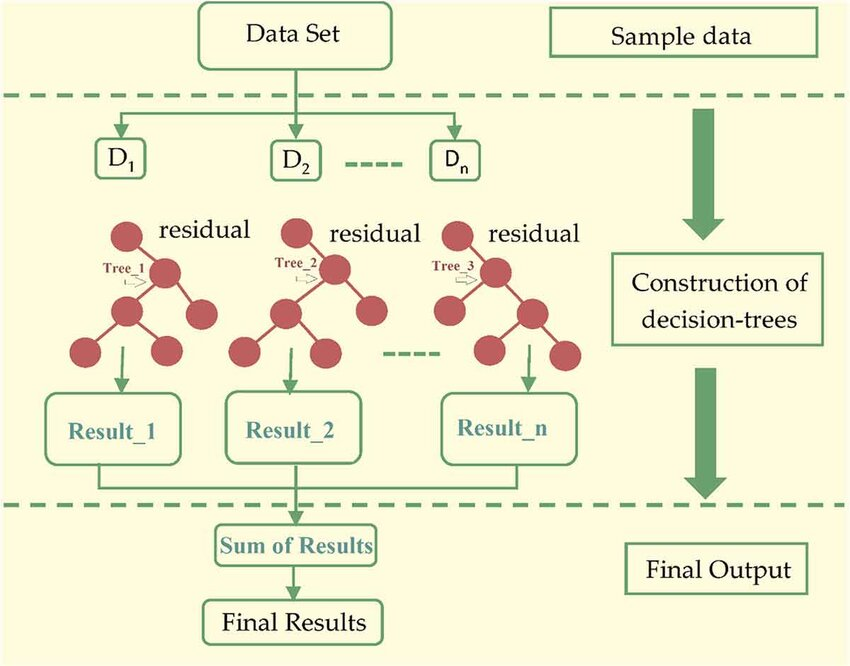
\includegraphics[width=0.8\textwidth]{img/xgb.png}
		\caption{Architettura del XGBoost.}
	\end{figure}
	
	\section{Introduzione al Gradient boosting}
	\begin{figure}[H]
		\centering
		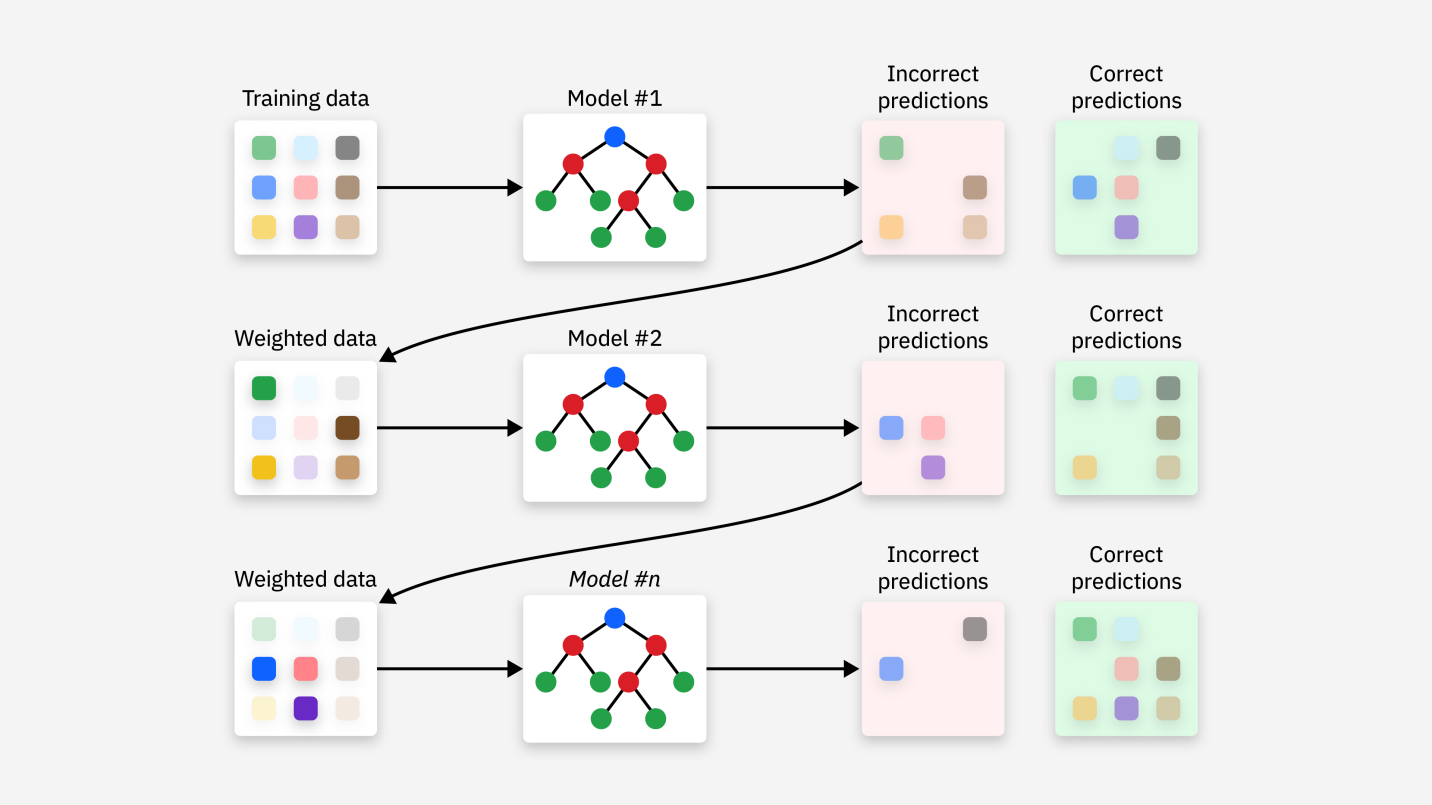
\includegraphics[width=1.0\textwidth]{img/grad_boost.png}
		\caption{Funzionamento del Gradient boosting.}
	\end{figure}
	
	Il Gradient boosting è una tecnica di Ensemble learning che costruisce un modello predittivo forte combinando iterativamente i risultati di numerosi "learner deboli". A differenza del Bagging, che addestra i modelli in parallelo, il Boosting adotta un approccio sequenziale, dove ogni nuovo modello cerca di correggere gli errori commessi dai modelli precedenti.
	
	\subsection{Principi iterativi e Weak learners}
	
	Il gradient boosting si fonda sull'idea di migliorare progressivamente un modello addestrando nuovi learner per correggere gli errori commessi dai precedenti. Questo processo è intrinsecamente iterativo e sequenziale. A differenza del Bagging, dove i learner sono addestrati in modo parallelo ed indipendente, il gradient boosting costruisce un modello additivo passo dopo passo. Ogni nuovo "albero" (che funge da learner debole) viene costruito specificamente per ridurre gli errori, o più precisamente gli "pseudo-residui", generati dalle previsioni degli alberi addestrati nelle iterazioni precedenti.
	I "learner deboli", in questo caso, sono modelli che, se utilizzati singolarmente, classificano o predicono i dati in modo scarso e presentano un alto tasso di errore. Nel framework del gradient boosting, i learner deboli sono tipicamente alberi di decisione semplici. Possono essere molto semplici, a volte ridotti ad un singolo split, in tal caso sono noti come "decision stumps". L'obiettivo generale del gradient boosting è minimizzare una funzione di perdita predefinita, aggiungendo iterativamente funzioni (i learner deboli) che puntano nella direzione del gradiente negativo di tale funzione. Mentre il Bagging mira a ridurre la varianza addestrando modelli indipendenti e poi mediandone i risultati, il Boosting si concentra sulla riduzione del bias del modello. Addestrando sequenzialmente nuovi learner per correggere gli errori dei precedenti, il modello impara a concentrarsi sulle istanze più difficili da classificare o predire. Questo processo iterativo consente al modello di adattarsi in modo più efficace alle relazioni complesse presenti nei dati, riducendo il bias complessivo e portando spesso a una maggiore accuratezza predittiva. Questa differenza fondamentale nell'approccio, ovvero la riduzione della varianza contro la riduzione del bias, spiega perché il Bagging ed il Boosting eccellono in contesti diversi.
	
	\subsection{Funzione di perdita e Discesa del gradiente}
	
	Il processo di apprendimento nel gradient boosting è formalizzato come un algoritmo di discesa del gradiente nello spazio delle funzioni, dove l'obiettivo è trovare la funzione che minimizza la funzione di perdita, che quantifica quanto bene il modello sta eseguendo le previsioni sui dati forniti. La scelta della funzione di errore dipende dalla natura del problema: ad esempio, per problemi di regressione si potrebbe usare l'errore quadratico medio (MSE), mentre per problemi di classificazione si potrebbe usare la log-loss. L'algoritmo di gradient boosting mira a minimizzare questa funzione di perdita. In ogni iterazione, il modello calcola i cosiddetti "pseudo-residui", che non sono i residui tradizionali (differenza tra valore osservato e previsto), ma piuttosto i gradienti negativi della funzione di perdita rispetto alle previsioni attuali del modello. Il nuovo learner debole (tipicamente un albero di decisione) viene quindi addestrato per predire questi pseudo-residui, imparando così a correggere gli errori del modello ensemble cumulativo. Il processo di aggiunta di nuovi alberi può essere interpretato come un passo nella direzione del gradiente negativo della funzione di perdita nello spazio delle funzioni. \\
	Un'innovazione significativa in XGBoost rispetto al gradient boosting tradizionale è l'utilizzo di un'approssimazione di Taylor del secondo ordine nella funzione di perdita. Questo approccio collega il processo di ottimizzazione di XGBoost al metodo Newton-Raphson, che è più robusto e può portare a una convergenza più rapida rispetto alla discesa del gradiente del primo ordine. L'utilizzo di un'approssimazione di Taylor del secondo ordine nella funzione di perdita distingue XGBoost dal gradient boosting tradizionale, che si basa sul gradiente del primo ordine. Ciò implica che XGBoost considera, non solo la direzione di discesa più ripida (data dal gradiente), ma anche la curvatura della funzione di perdita (data dall'hessiana). Ciò consente al modello di compiere passi più informati e potenzialmente più ampi verso il minimo della funzione di perdita, portando a una convergenza più rapida e stabile. Di conseguenza, XGBoost risulta meno sensibile a problemi come i minimi locali rispetto agli algoritmi che utilizzano esclusivamente il gradiente del primo ordine. Questa modifica è uno dei motivi principali della superiorità prestazionale di XGBoost in numerose competizioni di machine learning ed in svariate applicazioni reali. Dimostra come un'implementazione più avanzata dei principi fondamentali possa tradursi in miglioramenti significativi in termini di prestazioni ed efficienza del modello.
	
	\section{Miglioramenti di XGBoost rispetto al Gradient boosting tradizionale}
	
	XGBoost è riconosciuto come un'evoluzione del gradient boosting, grazie all'integrazione di una serie di ottimizzazioni e tecniche di regolarizzazione che ne migliorano significativamente prestazioni, velocità e robustezza.
	
	\subsection{Regolarizzazione e Tree pruning}
	XGBoost si distingue per l'integrazione di meccanismi di regolarizzazione configurabili, che sono cruciali per prevenire l'overfitting e migliorare la sua capacità di generalizzazione. Il modello incorpora termini di regolarizzazione L1 (Lasso) e L2 (Ridge) direttamente nella sua funzione obiettivo. Questi termini penalizzano la complessità del modello e i pesi di grandi dimensioni. In particolare, la regolarizzazione L1, che si basa sulla somma del valore assoluto dei pesi:
	$$ \Omega(w) = \lambda \|w\|_1 = \lambda \sum_j |w_j| $$
	incoraggia la sparsità, spingendo i pesi meno importanti verso lo zero. Al contrario, la regolarizzazione L2, che si basa sulla somma dei quadrati dei pesi:
	$$ \Omega(w) = \lambda \|w\|_2^2 = \lambda \sum_j w_j^2 $$
	incoraggia pesi più piccoli e distribuiti. \\
	Una componente fondamentale della regolarizzazione nel gradient boosting è il learning rate (o shrinkage). Questo parametro riduce il contributo di ogni nuovo albero aggiunto al modello. L'uso di learning rate piccoli (ad esempio, 0.01 o 0.1) migliora notevolmente la capacità di generalizzazione del modello, sebbene ciò comporti un aumento del numero di iterazioni e, di conseguenza, del tempo di calcolo. \\
	XGBoost implementa anche tecniche avanzate di tree pruning. A differenza di alcuni algoritmi che costruiscono alberi fino alla massima profondità, XGBoost pota gli alberi in base a un "guadagno" del nodo. La decisione di effettuare una ulteriore divisione su un nodo foglia dipende dal raggiungimento di un guadagno minimo, specificato dall'iperparametro $\gamma$ (gamma). Un valore più grande di $\gamma$ rende l'algoritmo più conservativo, limitando la crescita dell'albero e aiutando a prevenire l'overfitting.
	Il guadagno di un nodo in XGBoost quantifica il miglioramento nella funzione obiettivo che si ottiene dividendo un nodo. Questo guadagno deve superare una soglia minima, definita dall'iperparametro $\gamma$, per autorizzare la divisione. La formula per il guadagno è:
	$$
	\text{Gain} = \frac{1}{2} \left[ \frac{(\sum_{i \in I_L} g_i)^2}{\sum_{i \in I_L} h_i + \lambda} + \frac{(\sum_{i \in I_R} g_i)^2}{\sum_{i \in I_R} h_i + \lambda} - \frac{(\sum_{i \in I} g_i)^2}{\sum_{i \in I} h_i + \lambda} \right] - \gamma
	$$
	Dove $I_L$ e $I_R$ sono gli insiemi di istanze (dati di addestramento) nei nodi figli sinistro e destro, mentre $I$ rappresenta l'insieme di istanze nel nodo padre. In questa formula, $g_i$ è la derivata prima della funzione di perdita rispetto all'output dell'istanza $i$, mentre $h_i$ è la derivata seconda della funzione di perdita rispetto allo stesso output. Il parametro $\lambda$ è un termine di regolarizzazione L2 che penalizza i pesi elevati, e $\gamma$ è la soglia di guadagno minima richiesta per la divisione. Se il guadagno calcolato è inferiore a $\gamma$, la divisione viene annullata. \\
	Un altro parametro cruciale per la regolarizzazione è la somma minima dei pesi delle istanze, noto come "min\_child\_weight". Questo iperparametro agisce come un criterio di regolarizzazione per controllare la crescita degli alberi. Un nodo figlio può essere creato solo se la somma dei pesi delle istanze al suo interno supera un valore soglia predefinito. Questa somma è calcolata usando l'**hessiana**, e la condizione per uno split può essere espressa come:
	$$ \sum_{i \in I_L} h_i \ge \text{min\_child\_weight} \quad \text{e} \quad \sum_{i \in I_R} h_i \ge \text{min\_child\_weight} $$
	Se una delle somme è inferiore al valore di "min\_child\_weight", la partizione viene annullata. Un valore più grande di questo iperparametro rende l'algoritmo più conservativo, riducendo la complessità degli alberi individuali e aiutando a prevenire l'overfitting.
	
	\subsection{Gestione dei valori mancanti}
	
	XGBoost è in grado di lavorare efficacemente anche quando nel dataset ci sono dati assenti o non registrati per alcune feature. XGBoost incorpora internamente un meccanismo che permette di decidere automaticamente, durante la costruzione degli alberi, come trattare i valori mancanti. Durante la costruzione degli alberi di decisione, quando viene incontrato un valore mancante per una determinata feature, XGBoost non si limita a ignorare o richiedere una rimozione preliminare di essa. Invece, l'algoritmo impara quale direzione (ramo dell’albero) seguire per le istanze con valori mancanti per ottimizzare le performance. Internamente, durante la fase di training, XGBoost tratta la "mancanza" del dato come una caratteristica informativa a sé stante, apprendendo la direzione ottimale per i dati mancanti in modo da ottimizzare le suddivisioni. Questa capacità semplifica la pipeline di preparazione dei dati, evitando bias o rumori introdotti da imputazioni errate o rimozioni arbitrarie, e rende il modello più robusto e affidabile in scenari del mondo reale, dove i dati spesso presentano valori mancanti. Questa funzionalità rende XGBoost particolarmente efficiente e pratico per dataset reali, che spesso contengono valori mancanti, riducendo la necessità di avere una fase di pre-processing complessa, migliorando così l'affidabilità del modello in scenari del mondo reale.
	
	\subsection{Ottimizzazioni (Parallelismo, Cache-awareness)}
	
	Una delle ottimizzazioni chiave di XGBoost è il parallelismo. Sebbene il gradient boosting sia intrinsecamente sequenziale nella costruzione degli alberi (ogni albero corregge gli errori del precedente), XGBoost introduce il parallelismo, nella costruzione dei singoli alberi, in particolare sui livelli dell'albero o di split. Questo significa che, anziché costruire gli alberi in modo strettamente sequenziale, XGBoost può scansionare i valori del gradiente ed utilizzare somme parziali per valutare la qualità degli split in parallelo. Il sistema sfrutta tutti i core della CPU disponibili su una singola macchina e può operare in modalità distribuita, massimizzando l'utilizzo della potenza di calcolo. Questo parallelismo su larga scala accelera significativamente il processo di addestramento. \\
	Un'altra ottimizzazione interessante è il Cache-awareness. XGBoost è progettato per utilizzare in modo intelligente la cache della CPU per accelerare l'accesso ai dati. Durante l'addestramento, memorizza nella cache i calcoli intermedi e le statistiche importanti, evitando così di ricalcolare gli stessi valori ripetutamente. Questo riduce i ritardi nel recupero dei dati tra la CPU e memoria principale, portando ad un'elaborazione e previsioni molto più veloci. \\
	Infine, XGBoost beneficia della GPU acceleration, che velocizza significativamente l'addestramento del modello e contribuisce a migliorare l'accuratezza delle previsioni. L'algoritmo sfrutta il calcolo parallelo per eseguire operazioni veloci, per ripartizionare i dati e costruire gli alberi un livello alla volta, elaborando l'intero dataset contemporaneamente sulla GPU. \\
	
	\section{Parametri chiave e Tuning}
	
	XGBoost offre un'ampia e dettagliata lista di iperparametri che possono essere ottimizzati per personalizzare il comportamento del modello e massimizzare le sue prestazioni. Questa flessibilità, sebbene potente, richiede una comprensione approfondita ed un'attenta strategia di tuning.
	I parametri per il Tree booster controllano la costruzione dei singoli alberi all'interno dell'Ensemble:
	\begin{itemize}
		\item \texttt{learning\_rate} (o \texttt{eta}): questo è il tasso di apprendimento, un parametro cruciale che controlla la dimensione del passo di shrinkage per prevenire l'overfitting. Valori più piccoli di \texttt{eta} rendono il processo di boosting più conservativo, riducendo il rischio di overfitting ma richiedendo più iterazioni. Il suo intervallo è $(0, 1]$.
		\item \texttt{max\_depth}: definisce la profondità massima di un albero. Aumentare questo valore rende il modello più complesso e potenzialmente più incline all'overfitting. Un valore di $0$ indica nessuna limitazione di profondità, ma ciò può portare a un elevato consumo di memoria. L'intervallo è $[0, \infty]$.
		\item \texttt{min\_child\_weight}: specifica la somma minima del peso delle istanze (basata sull'hessiana) necessaria in un nodo figlio per consentire un ulteriore split. Un valore più grande rende l'algoritmo più conservativo, limitando la crescita dell'albero. L'intervallo è $[0, \infty]$.
		\item \texttt{subsample}: rappresenta la frazione di osservazioni (istanze) campionate casualmente per la costruzione di ogni albero. Questo campionamento avviene una volta per ogni iterazione di boosting ed aiuta a prevenire l'overfitting. L'intervallo è $(0, 1]$.
		\item \texttt{colsample\_bytree}: indica la frazione di features campionate casualmente per la costruzione di ogni albero. Questo parametro contribuisce anch'esso a prevenire l'overfitting introducendo casualità nella selezione delle caratteristiche. L'intervallo è $(0, 1]$.
		\item \texttt{lambda} (o \texttt{reg\_lambda}): é il termine di regolarizzazione L2 sui pesi. Aumentare questo valore rende il modello più conservativo, penalizzando i pesi grandi. L'intervallo è $[0, \infty)$.
		\item \texttt{alpha} (o \texttt{reg\_alpha}): é il termine di regolarizzazione L1 sui pesi. Un valore più grande rende il modello più conservativo e incoraggia la sparsità, spingendo i pesi meno importanti verso lo zero. L'intervallo è $[0, \infty]$.
		\item \texttt{objective}: definisce la funzione obiettivo che il modello mira a minimizzare. Ad esempio, \texttt{reg:squarederror} per problemi di regressione, \texttt{binary:logistic} per classificazione binaria e \texttt{multi:softprob} per classificazione multiclasse.
		\item \texttt{eval\_metric}: specifica la metrica di valutazione da monitorare durante l'addestramento. È possibile specificare più metriche.
	\end{itemize}
	A differenza di Random forest, che tende ad avere meno parametri da ottimizzare, XGBoost richiede una comprensione più approfondita ed una sperimentazione più estesa per raggiungere le sue prestazioni ottimali. Questo implica che, sebbene XGBoost possa teoricamente superare Random forest in termini di accuratezza, raggiungere tale superiorità richiede un investimento maggiore in termini di tempo e risorse per il tuning.
	
	\section{Vantaggi}
	
	L'algoritmo XGBoost è rinomato per le sue prestazioni e si distingue per una serie di vantaggi chiave che lo rendono uno standard nel machine learning competitivo. Uno dei suoi punti di forza principali è \textbf{la robustezza all'overfitting}, garantita da varie tecniche di regolarizzazione integrate. Questo controllo granulare sulla complessità del modello è un fattore determinante per la sua notevole capacità di generalizzazione. \\
	XGBoost è stato progettato per la scalabilità e l'efficienza, permettendogli \textbf{una gestione efficiente di grandi dataset}, dati sparsi e valori mancanti. La sua architettura ottimizzata consente di elaborare volumi di dati che per altri algoritmi sarebbero difficili da gestire. Nonostante la sua natura sequenziale, \textbf{la velocità di addestramento} di XGBoost è eccezionale; può superare quella del Random Forest, specialmente quando si sfruttano le sue capacità di parallelismo e l'accelerazione GPU, oltre al supporto per sistemi distribuiti. \\
	Un altro vantaggio significativo è \textbf{la sua flessibilità e personalizzazione}. L'algoritmo offre un'ampia gamma di iperparametri che consentono un fine-tuning profondo, adattando il modello alle specifiche esigenze di ogni problema e dataset. Inoltre, XGBoost è particolarmente efficace nella \textbf{gestione di dati sbilanciati}, un problema comune in molti contesti di classificazione.
	
	\section{Svantaggi}
	
	Nonostante i suoi punti di forza, XGBoost presenta alcune limitazioni, principalmente legate alla sua complessità. \textbf{Il processo di addestramento sequenziale} può renderlo intrinsecamente più lento del Random Forest nella costruzione completa degli alberi, dato che ogni albero dipende dal precedente. Sebbene siano state introdotte ottimizzazioni per il parallelismo interno, la sua natura sequenziale rimane una potenziale barriera, a meno che non si sfruttino appieno le sue capacità di parallelismo e le accelerazioni hardware. \\
	\textbf{La complessità e la necessità di tuning} rappresentano un'altra sfida. XGBoost è un algoritmo più complesso da comprendere e implementare rispetto al Random Forest. La sua vasta gamma di iperparametri richiede una maggiore conoscenza ed esperienza per un fine-tuning efficace, rendendo il processo più dispendioso in termini di tempo e risorse. \\
	Inoltre, XGBoost può risultare \textbf{meno interpretabile del Random Forest}. Sebbene fornisca l'importanza delle feature, la complessità dell'ensemble di alberi sequenziali può rendere le sue decisioni specifiche più difficili da interpretare. Spesso sono necessari strumenti aggiuntivi per la spiegabilità, a differenza del Random Forest che, in alcuni casi, può essere più trasparente. \\
	Infine, \textbf{il consumo di memoria} può essere una limitazione significativa. XGBoost può consumare una notevole quantità di memoria, in particolare quando si addestrano alberi molto profondi. Questo può rappresentare un problema per dataset estremamente grandi su hardware con risorse limitate.
	
	\chapter{Convolutional Neural Networks (CNN)}
	
	\section{Introduzione}
	Questo capitolo si occupa di introdurre le Convolutional Neural Networks (CNN), un'architettura di rete neurale che eccelle nell'analisi di immagini e di dati con una struttura a griglia. L'obiettivo è esplorare come queste reti riescano ad estrarre automaticamente le caratteristiche rilevanti, superando i limiti delle reti tradizionali. Il testo descriverà il funzionamento dei principali blocchi costruttivi, come la convoluzione e il pooling, che permettono alla rete di identificare forme e pattern in modo gerarchico e di ridurne la complessità. Verrà poi spiegato come, attraverso una sequenza di operazioni, un'immagine viene trasformata in rappresentazioni via via più astratte fino a giungere ad una decisione finale. Infine, il capitolo riassume i vantaggi delle CNN, come la loro efficienza e la capacità di riconoscere oggetti a prescindere dalla loro posizione, e i loro svantaggi, tra cui la necessità di enormi quantità di dati e il loro costo computazionale. \cite{oshea2015cnn, krizhevsky2012imagenet, simonyan2014very, ioffe2015batch, ba2016layer, wu2018group, poojary2020dataaug}
	
	\begin{figure}[H]
		\centering
		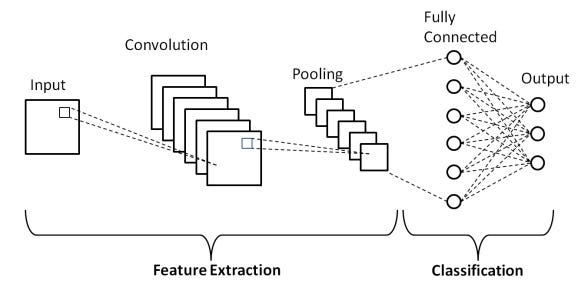
\includegraphics[width=1.0\textwidth]{img/cnn.jpg}
		\caption{Architettura delle Convolutional Neural Networks.}
	\end{figure}
	
	\section{Principi fondamentali delle CNN}
	
	\subsection{Convoluzione: kernel, stride, padding}
	Un kernel (o filtro) è una matrice di piccole dimensioni, tipicamente 3$\times$3, 5$\times$5 o 7$\times$7, contenente pesi apprendibili che vengono moltiplicati elemento per elemento con porzioni locali dell'input. Durante l'operazione di convoluzione, il kernel viene fatto scorrere attraverso l'intera immagine di input, calcolando il prodotto scalare tra i pesi del filtro e i valori corrispondenti dell'input in ogni posizione. \\
	Lo stride rappresenta la grandezza in pixel di cui il kernel si sposta ad ogni passo durante la convoluzione. Uno stride di 1 significa che il filtro si muove di un pixel alla volta, producendo un output con dimensioni spaziali simili all'input. Uno stride maggiore (ad esempio 2 o 3) riduce significativamente le dimensioni dell'output, fornendo un effetto di downsampling. \\
	Il padding è una tecnica che consiste nell'aggiungere pixel (solitamente con valore zero) ai bordi dell'immagine di input. Esistono due tipi principali di padding:
	\begin{itemize}
		\item Valid padding: nessun padding viene aggiunto, l'output risulta più piccolo dell'input.
		\item Same padding: viene aggiunto padding sufficiente per mantenere le stesse dimensioni spaziali dell'input.
	\end{itemize}
	La formula per calcolare le dimensioni dell'output di una convoluzione è:
	$$O = \frac{W - K + 2P}{S} + 1$$
	dove $W$ è la dimensione dell'input, $K$ è la dimensione del kernel, $P$ è il padding e $S$ è lo stride.
	
	\subsection{Feature maps e profondità dei canali}
	Le feature maps rappresentano l'output prodotto dall'applicazione di filtri convoluzionali all'input. Ogni feature map corrisponde ad un filtro specifico e rappresenta la risposta di quel filtro all'immagine di input. Negli strati iniziali della rete, le feature maps possono catturare caratteristiche semplici come bordi, linee e angoli, mentre negli strati più profondi possono rappresentare pattern più complessi come forme, texture o addirittura oggetti interi. \\
	La profondità dei canali si riferisce al numero di feature maps prodotte da uno strato convoluzionale. Aumentare il numero di feature maps consente alla rete di apprendere caratteristiche più complesse e astratte, ma incrementa anche il costo computazionale e può portare ad overfitting se la rete è troppo grande per i dati disponibili. Un aspetto cruciale è che la profondità di un filtro deve corrispondere alla profondità dell'input. Ad esempio, per un'immagine RGB (3 canali), ogni filtro deve avere profondità 3. L'output di ogni convoluzione è una feature map 2D, indipendentemente dalla profondità dell'input.
	
	\section{Pooling e normalizzazione}
	
	\subsection{Max pooling vs average pooling}
	Il pooling è un'operazione di downsampling che riduce le dimensioni spaziali delle feature maps mantenendo le informazioni più importanti. Questa operazione migliora l'efficienza computazionale e introduce una forma di invarianza alle traslazioni, rendendo la rete meno sensibile a piccoli spostamenti nell'input. \\
	Il max pooling seleziona il valore massimo all'interno di ogni finestra di pooling. È particolarmente efficace nel preservare le caratteristiche più importanti e nell'introdurre invarianza alle traslazioni. Ad esempio, con una finestra 2$\times$2 e stride 2, il max pooling riduce le dimensioni dell'input della metà mantenendo le attivazioni più forti. \\
	L'average pooling calcola la media dei valori all'interno di ogni finestra di pooling. Mentre preserva più informazione locale rispetto al max pooling, può essere meno efficace nel gestire variazioni sottili delle caratteristiche o features significative in certe regioni dell'immagine.
	
	\subsection{Global pooling}
	
	Il global pooling è una variante che riduce ogni feature map ad un singolo valore, eliminando completamente le dimensioni spaziali. Il global max pooling seleziona il valore massimo da ogni feature map intera, mentre il global average pooling calcola la media di tutti i valori in ogni feature map. Questa tecnica è spesso utilizzata prima degli strati fully connected finali nelle architetture CNN per la classificazione, riducendo drasticamente il numero di parametri e prevenendo l'overfitting.
	
	\subsection{Batch, Layer e Group normalization}
	La batch normalization è una tecnica introdotta per accelerare l'addestramento delle reti neurali profonde e ridurre la sensibilità all'inizializzazione dei parametri. Normalizza gli input di ogni strato utilizzando la media e varianza del mini-batch corrente durante l'addestramento. \\
	Per ogni canale, durante la fase di apprendimento, la batch normalization calcola:
	$$\hat{x}_i = \frac{x_i - \mu_B}{\sqrt{\sigma_B^2 + \epsilon}}$$
	dove $\mu_B$ e $\sigma_B^2$ sono la media e varianza del batch, ed $\epsilon$ è una costante piccola per evitare divisioni per zero. Successivamente applica una trasformazione affine apprendibile:
	$$y_i = \gamma \hat{x}_i + \beta$$
	dove $\gamma$ e $\beta$ sono parametri apprendibili. \\
	La layer normalization normalizza tutti i neuroni in un particolare strato per ogni input individualmente, rendendola indipendente dalla dimensione del batch. \\
	La group normalization divide i canali in gruppi e normalizza all'interno di ogni gruppo, offrendo un compromesso tra batch e layer normalization.
	
	\section{Data augmentation: rotazioni, zoom, colour jitter}
	La data augmentation è una tecnica che aumenta artificialmente le dimensioni del dataset applicando trasformazioni realistiche agli esempi di training, migliorando la generalizzazione e riducendo l'overfitting. \\
	Le rotazioni ruotano le immagini di angoli casuali (tipicamente tra -50$^\circ$ e 50$^\circ$), aiutando la rete a riconoscere oggetti indipendentemente dal loro orientamento. Studi hanno dimostrato che la rotazione può migliorare significativamente le prestazioni. \\
	Lo zoom (o scaling) modifica le dimensioni degli oggetti nell'immagine, permettendo alla rete di riconoscere oggetti a diverse scale. Il random crop è una variante che estrae porzioni casuali dell'immagine originale. \\
	Il colour jitter modifica luminosità, contrasto, saturazione e tonalità delle immagini. Questa tecnica varia i canali RGB con valori casuali, producendo cambiamenti casuali nel colore che aiutano la rete a essere invariante alle variazioni di illuminazione e colore.
	
	\section{Funzionamento delle CNN}
	
	\subsection{Forward pass}
	\begin{figure}[H]
		\centering
		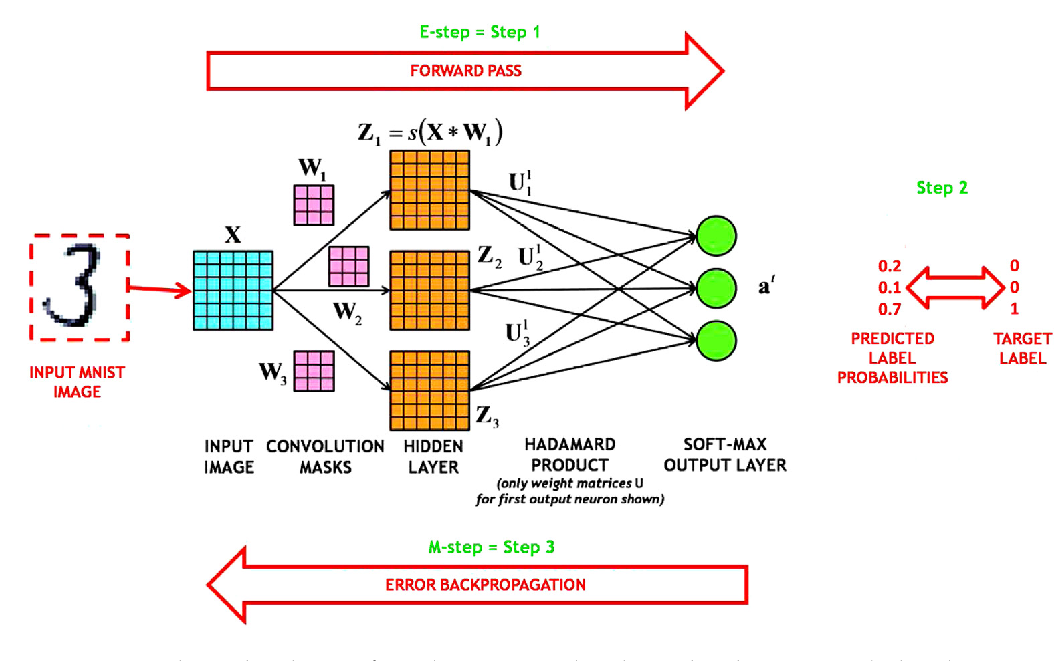
\includegraphics[width=1.0\textwidth]{img/cnn_fp.png}
		\caption{Diagramma del forward pass in una CNN.}
	\end{figure}
	Il forward pass rappresenta il percorso che i dati seguono dall’input verso l’output attraverso l’intera architettura della rete. Questo processo inizia con l’immagine grezza e termina con la predizione finale, passando attraverso una serie di trasformazioni matematiche che estraggono progressivamente caratteristiche sempre più complesse.
	
	\subsection{Strati di convoluzione}
	Il primo stadio, per l'elaborazione delle immagini, coinvolge gli strati convoluzionali, che rappresentano il cuore dell’architettura CNN. Quando un’immagine di input entra nella rete, essa viene elaborata attraverso un insieme di filtri (kernel) che eseguono l’operazione di convoluzione. Ogni filtro è responsabile del rilevamento di una specifica caratteristica: negli strati iniziali, questi filtri apprendono a riconoscere caratteristiche di basso livello come bordi, linee e angoli. L’operazione di convoluzione produce le feature maps, che rappresentano la risposta di ciascun filtro all’immagine di input. Ogni elemento nella feature map indica l’intensità della presenza di quella specifica caratteristica in quella posizione dell’immagine.
	
	\subsection{Funzioni di attivazione}
	Dopo ogni operazione di convoluzione, viene applicata una funzione di attivazione, tipicamente ReLU. Questa fase è cruciale perché introduce non-linearità nel modello, permettendo alla rete di apprendere relazioni complesse nei dati.
	
	\subsection{Strati di pooling}
	Successivamente agli strati convoluzionali, i dati passano attraverso gli strati di pooling. Questi strati eseguono un’operazione di downsampling che riduce le dimensioni spaziali delle feature maps mantenendo le informazioni più importanti.
	
	\subsection{Gerarchia delle caratteristiche}
	Man mano che i dati attraversano strati successivi, si verifica un fenomeno fondamentale: la costruzione gerarchica delle caratteristiche. Gli strati iniziali rilevano caratteristiche elementari (bordi, texture), gli strati intermedi combinano queste caratteristiche per formare pattern più complessi (forme geometriche, motivi), mentre gli strati più profondi assemblano questi pattern in rappresentazioni di alto livello che corrispondono a parti di oggetti o oggetti interi.
	
	\subsection{Strati fully-connected}
	Dopo l'estrazione gerarchica delle caratteristiche, i dati raggiungono gli strati fully-connected. Prima di entrare in questi strati, le mappe di caratteristiche multidimensionali vengono convertite in un vettore unidimensionale. Negli strati fully-connected, ogni neurone è collegato a tutti i neuroni dello strato precedente, consentendo alla rete di combinare tutte le caratteristiche estratte per prendere la decisione finale, in base al tipo di problema. \\
	Durante il terzo caso di studio, verranno esplorate le modifiche agli strati fully-connected delle CNN, analizzando due diverse architetture: MLP e KAN.
	
	\subsection{Flusso informativo e Trasformazioni progressive}
	Durante tutto questo processo, l’immagine originale, inizialmente rappresentata come una matrice di valori pixel, viene gradualmente trasformata in rappresentazioni sempre più astratte e significative dal punto di vista semantico. Ogni strato della rete contribuisce a questa trasformazione: gli strati convoluzionali estraggono e raffinano le caratteristiche, gli strati di pooling riducono la complessità computazionale e introducono invarianza, mentre gli strati fully-connected integrano tutte le informazioni per la classificazione finale. \\
	Questo design architetturale permette alle CNN di apprendere automaticamente le rappresentazioni ottimali per il compito specifico, eliminando la necessità di progettare manualmente gli estrattori di caratteristiche. La capacità di costruire rappresentazioni gerarchiche rende le CNN particolarmente efficaci per compiti di computer vision, dove la comprensione dell’immagine richiede l’integrazione di informazioni a diversi livelli di astrazione.
	
	\section{Vantaggi}
	
	Le CNN si distinguono per una serie di vantaggi che le rendono lo standard per l'elaborazione delle immagini. Il loro punto di forza principale è il \textbf{rilevamento automatico delle caratteristiche}. A differenza delle reti neurali tradizionali che richiedono un'estrazione manuale delle feature, le CNN apprendono e identificano autonomamente le caratteristiche rilevanti direttamente dai dati grezzi. Questo approccio riduce drasticamente lo sforzo di pre-processing e permette al modello di adattarsi in modo più efficace ai dati. \\
	Un'altra caratteristica distintiva è la loro \textbf{efficienza computazionale e riduzione dei parametri}. L'uso del weight sharing (una tecnica che permette ad un singolo filtro di rilevare la stessa caratteristica in qualsiasi posizione dell'immagine utilizzando lo stesso set di pesi) e degli strati di pooling riduce notevolmente il numero di parametri da addestrare rispetto alle reti fully-connected. Questo non solo accelera l'addestramento, ma contribuisce anche a prevenire l'overfitting. \\
	Grazie all'operazione di convoluzione, le CNN offrono \textbf{invarianza alla traslazione}. Sono in grado di riconoscere un oggetto indipendentemente dalla sua posizione nell'immagine. Un filtro che ha imparato a riconoscere un occhio, ad esempio, lo riconoscerà sia che si trovi in alto a sinistra che in basso a destra. \\
	Le architetture CNN sono anche estremamente \textbf{scalabili}: possono essere adattate facilmente a dataset di grandi dimensioni ed a compiti complessi, aumentando la profondità e la larghezza della rete per gestire immagini ad alta risoluzione o per apprendere pattern più astratti.
	
	\section{Svantaggi}
	
	Nonostante i loro numerosi vantaggi, le CNN presentano alcune limitazioni. La principale è la loro \textbf{dipendenza da grandi dataset}. Specialmente le architetture più complesse richiedono enormi quantità di dati etichettati per un addestramento efficace. La mancanza di un dataset sufficientemente grande può portare all'overfitting o ad una scarsa capacità di generalizzazione. \\
	Un altro limite è l'\textbf{invarianza limitata}. Le CNN standard sono invarianti alla traslazione, ma non lo sono rispetto ad altre trasformazioni geometriche. Se un'immagine viene ruotata o scalata in modo significativo, il modello potrebbe non riconoscerla correttamente, a meno che non si usino tecniche di data augmentation per esporre il modello a tali variazioni durante l'addestramento. \\
	Le CNN sono spesso criticate per la loro \textbf{mancanza di interpretazione}. È difficile capire il motivo per cui un modello prenda una determinata decisione. Le feature map intermedie possono essere visualizzate, ma il processo decisionale complessivo rimane una "black box", rendendo complicato il debugging e l'adozione in settori critici come la medicina, dove è essenziale la trasparenza. \\
	Infine, l'addestramento di architetture CNN molto profonde ha un elevato \textbf{costo computazionale}. Spesso richiede una notevole potenza di calcolo e hardware specializzato come le GPU. Anche l'inferenza su dispositivi a bassa potenza può risultare problematica.
	
	\chapter{Ottimizzazione degli iperparametri}
	
	\section{Introduzione}
	Questo capitolo presenta una panoramica delle metodologie di ottimizzazione degli iperparametri, essenziali per migliorare le performance dei modelli di Machine e Deep Learning. L'obiettivo è esplorare come queste tecniche permettano di navigare lo spazio delle configurazioni di un modello per trovare la combinazione ideale. Il testo inizia descrivendo diverse forme di Cross-Validation, tra cui la K-fold CV, la Nested Cross-Validation e la Time Series Cross-Validation, pensata specificamente per i dati temporali. Successivamente, il capitolo si concentra sulle strategie di ricerca, a partire dai metodi più semplici come il Grid Search e il Random Search, per poi introdurre approcci più sofisticati come l'Ottimizzazione Bayesiana e gli Algoritmi Genetici. Infine, viene fornito un confronto pratico tra questi metodi per aiutare a comprendere quando applicare ciascuno di essi. Per la sua efficienza e scalabilità, in questa ricerca è stato scelto il Random Search, che è stato ottimizzato utilizzando una formula che utilizza le probabilità per determinare il numero ideale di iterazioni. \cite{franceschi2024hyperparameter, wainer2018cvncv, deng2023tscv, bergstra2012random, snoek2012bo, alibrahim2021gagsbo}
	
	\section{Cross-Validation (CV)}
	\begin{figure}[H]
		\centering
		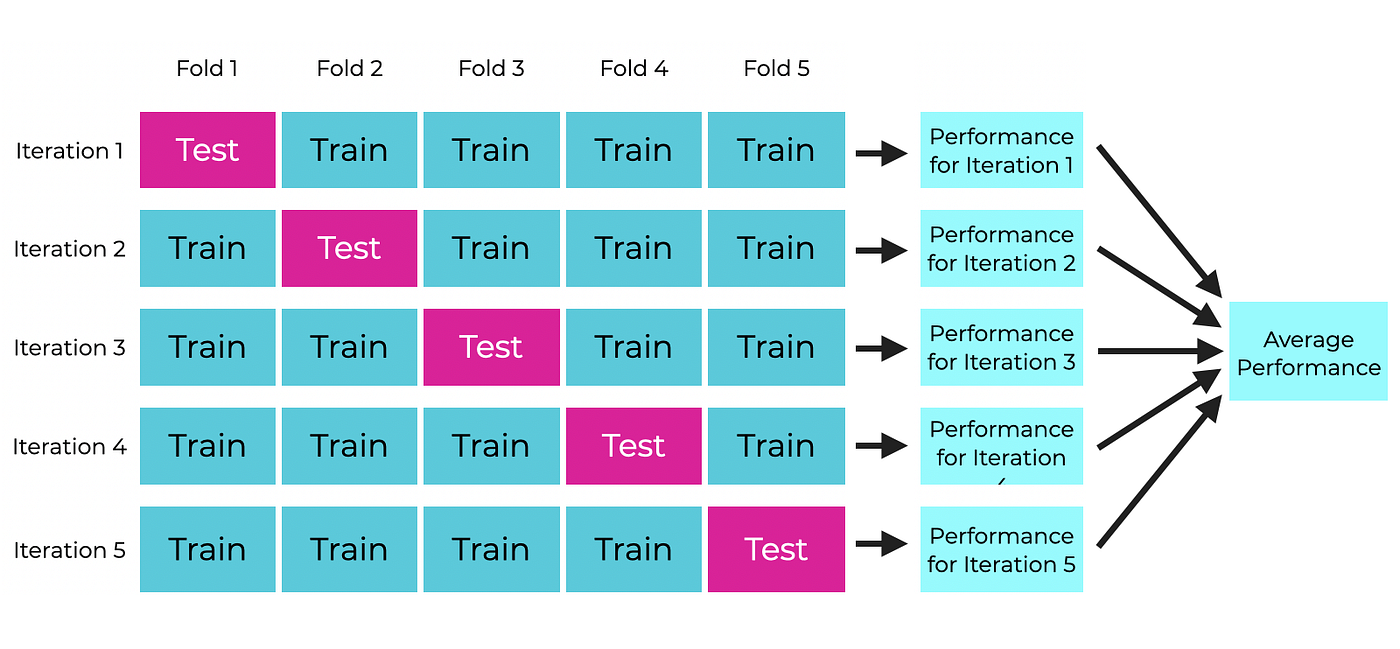
\includegraphics[width=1.0\textwidth]{img/cv.png}
		\caption{Funzionamento della tecnica di Cross-Validation.}
	\end{figure}
	La CV è una metodologia utilizzata per la valutazione delle prestazioni di un modello predittivo. Il suo scopo principale è quello di stimare quanto un modello é in grado di generalizzare su dati indipendenti non visti durante la fase di training. Dato un dataset $D = \{z_1, \dots, z_N\}$ e una procedura di training che produce un modello $\hat f_{D}$, la K-fold cross-validation divide i dati in $K$ parti disgiunte (fold), dove ognuno ha una dimensione approssimativamente uguale. Il processo si ripete $K$ volte. Per ogni iterazione $k \in \{1, \dots, K\}$, si usano le restanti $K-1$ parti, che costituiscono il training set $D^{(k)} = D \setminus D_k$, per allenare il modello. Questo produce un modello parziale $\hat f_{D^{(k)}}$. Poi, si valuta l'errore del modello $\hat f_{D^{(k)}}$ sul fold lasciato fuori $D_k$, che ricopre il ruolo del validation set per questa iterazione. L'errore viene calcolato come $E_k = \text{Errore}(\hat f_{D^{(k)}}, D_k)$. Al termine delle $K$ iterazioni, si ottiene una lista di $K$ errori $\{E_1, E_2, \dots, E_K\}$. La stima finale della performance del modello è data dalla media degli errori calcolati su ogni fold, $\bar{E} = \frac{1}{K} \sum_{k=1}^K E_k$.
	
	\subsection{Time Series Cross-Validation (TSCV)}
	\begin{figure}[H]
		\centering
		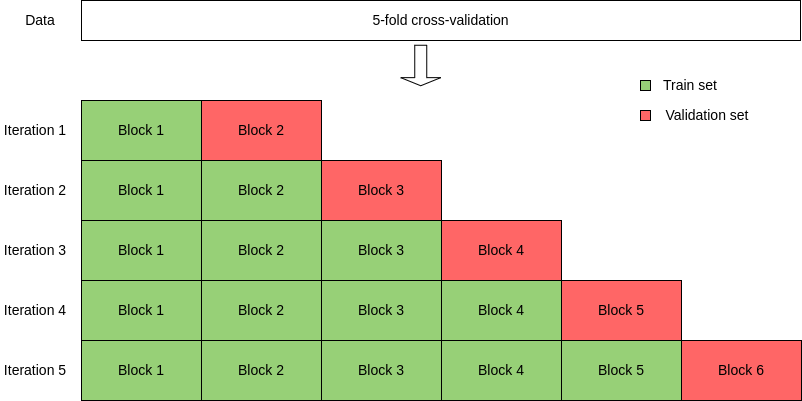
\includegraphics[width=1.0\textwidth]{img/tscv.png}
		\caption{Svolgimento della tecnica di Time Series Cross-Validation.}
	\end{figure}
	Per i dati che hanno una dipendenza temporale, come le serie storiche, la CV standard non è adatta. Suddividere i dati in fold casuali romperebbe la struttura temporale, e l'addestramento su dati futuri per testare il modello su dati passati (fenomeno noto come data leakage) non avrebbe senso pratico e porterebbe a risultati fuorvianti. La TSCV, sviluppata per risolvere questa problematica, crea un training set che cresce sequenzialmente nel tempo, ed il validation set è sempre un blocco di dati che segue immediatamente il dataset di allenamento. Il processo funziona così:
	\begin{itemize}
		\item \textbf{Prima iterazione:} il modello è addestrato sui primi $m$ punti temporali e testato sui successivi $n$ punti.
		\item \textbf{Seconda iterazione:} il modello è addestrato sui primi $m+n$ punti temporali e testato sui successivi $n$ punti.
		\item \textbf{Iterazioni successive:} il processo continua, con il training set che si espande ad ogni passo ed il validation set che avanza nel tempo.
	\end{itemize}
	Questo approccio rispecchia fedelmente lo scenario reale in cui un modello di serie storica viene addestrato su dati passati e utilizzato per fare previsioni su dati futuri non ancora visti. La media degli errori di validazione su tutte le iterazioni fornisce una stima robusta e realistica delle prestazioni del modello.
	
	\section{Nested Cross-Validation (NCV)}
	\begin{figure}[H]
		\centering
		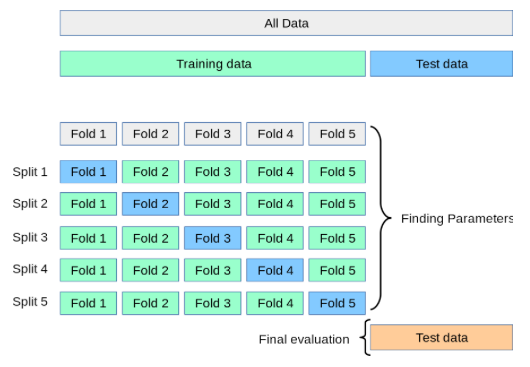
\includegraphics[width=1.0\textwidth]{img/ncv.png}
		\caption{Funzionamento della tecnica di Nested Cross-Validation.}
	\end{figure}
	La NCV é un estensione della classica CV. Il suo scopo principale è quello di fornire una stima imparziale ed affidabile dell'errore di generalizzazione di un modello, risolvendo il problema del bias di selezione che può verificarsi quando gli stessi dati vengono utilizzati sia per la scelta degli iperparametri che per la valutazione finale del modello. L'idea alla base della NCV è quella di creare due cicli di CV: un ciclo esterno ed uno interno. 
	
	\begin{enumerate}
		\item \textbf{Ciclo esterno (Outer loop):} ha il compito di stimare l'errore di generalizzazione del modello. Il dataset viene diviso in $K$ fold. Per ogni iterazione di questo ciclo, vengono utilizzati $K-1$ parti per costruire il training set esterno ed il restante fold agisce da test set finale, che non verrà mai utilizzato per la selezione degli iperparametri, garantendo una valutazione finale imparziale.
		\item \textbf{Ciclo interno (Inner loop):} all'interno di ogni iterazione del ciclo esterno, si esegue un altro ciclo di CV (solitamente con $L$ fold) sul training set esterno. Questo ciclo interno è dedicato esclusivamente all'ottimizzazione degli iperparametri. Per ogni combinazione di essi da testare (ad esempio, utilizzando Grid o Random Search), si addestra il modello sui $L-1$ fold interni e si valuta la sua performance sul fold interno rimanente. La combinazione di iperparametri che ottiene la migliore performance media su tutte le $L$ iterazioni viene selezionata.
		\item \textbf{Valutazione del modello ottimizzato:} una volta trovata la migliore combinazione di iperparametri nel ciclo interno, il modello viene addestrato nuovamente sull'intero training set esterno utilizzando proprio quella combinazione ottimale. Infine, la performance di questo modello viene valutata sul test set esterno, che é stato lasciato fuori all'inizio dell'iterazione $K$. L'errore ottenuto in questa fase è la stima delle prestazioni di generalizzazione del modello per quella specifica iterazione del ciclo esterno.
	\end{enumerate}
	Questo processo viene ripetuto per tutti i $K$ fold del ciclo esterno. La stima finale dell'errore del modello è la media dei $K$ errori ottenuti sui test set esterni.
	
	\section{Grid search (GS)}
	\begin{figure}[H]
		\centering
		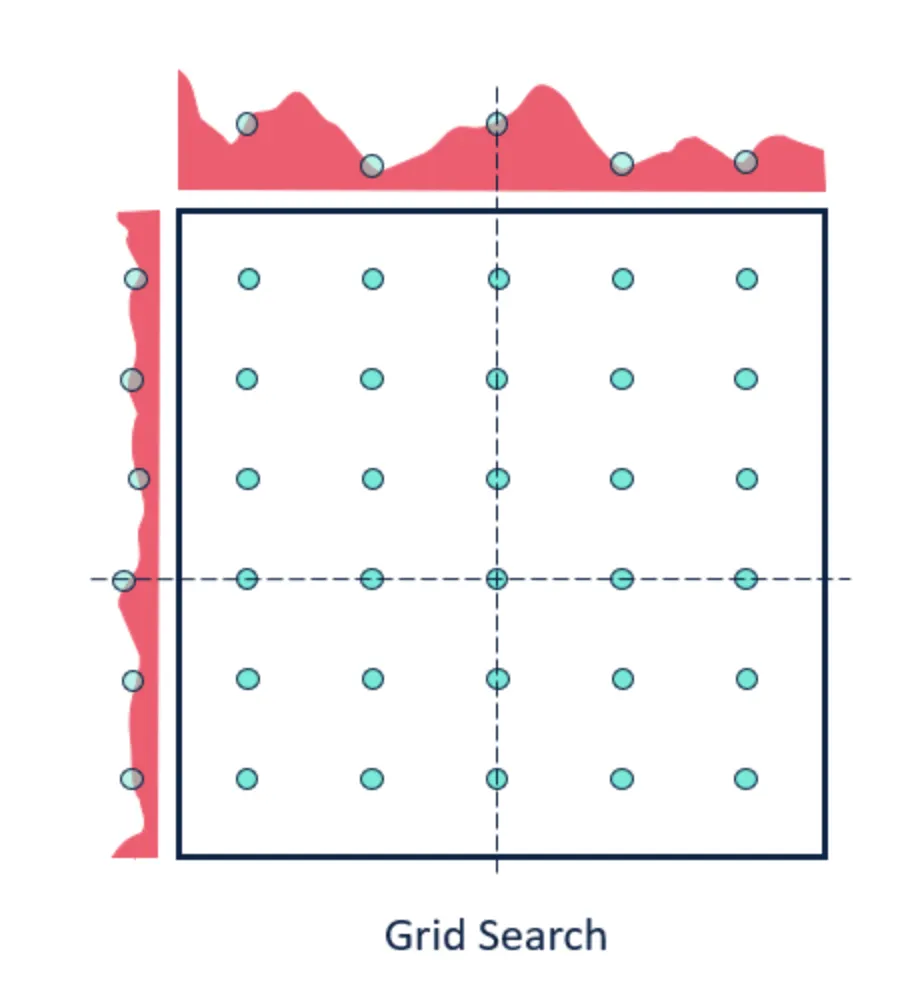
\includegraphics[width=1.0\textwidth]{img/gs.png}
		\caption{Grafico che mostra come Grid search ispeziona lo spazio degli iperparametri.}
	\end{figure}
	\subsection{Spiegazione dell'algoritmo}
	Il GS consiste nel definire una griglia discreta di possibili valori per ciascun iperparametro e nell'eseguire una valutazione esaustiva del modello per ogni combinazione. Alla fine, si seleziona il set di iperparametri che ottimizza la metrica di interesse. Il metodo non introduce casualità, risultando completamente ripetibile e deterministico.
	
	\subsection{Vantaggi}
	L'approccio del Grid Search offre diversi vantaggi. Primo fra tutti, la sua natura \textbf{esaustiva}: esplora tutte le combinazioni predefinite nello spazio di ricerca, permettendo di trovare l'ottimo globale se questo è incluso nella griglia. Inoltre, è un metodo \textbf{deterministico e riproducibile}, dato che l'assenza di casualità assicura che ogni esecuzione dell'algoritmo fornisca risultati replicabili. Infine, la sua \textbf{semplicità di implementazione} lo rende ideale in spazi di ricerca ridotti e ben definiti, o come baseline quando si dispone di elevate risorse computazionali.
	
	\subsection{Limiti}
	Nonostante i suoi vantaggi, il Grid Search presenta anche dei limiti significativi. Il suo \textbf{costo computazionale è esponenziale}, a causa della curse of dimensionality, rendendolo impraticabile per spazi di ricerca ampi o ad alta dimensionalità. Il metodo è spesso \textbf{inefficiente}, poiché molte valutazioni potrebbero riguardare regioni poco promettenti, specialmente quando solo alcuni parametri influenzano la performance ottimale. \textbf{La discretizzazione e la perdita di ottimi} sono altri problemi rilevanti: la necessità di fissare una griglia per iperparametri continui può portare a saltare valori potenzialmente migliori che non sono inclusi. Infine, non è \textbf{adatto a modelli e dataset complessi}, poiché il costo aumenta drasticamente con la complessità e la dimensione del dataset.
	
	\section{Random Search (RS)}
	\begin{figure}[H]
		\centering
		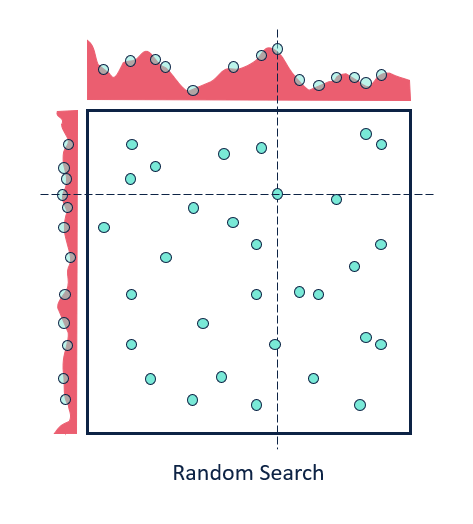
\includegraphics[width=1.0\textwidth]{img/rs.png}
		\caption{Grafico che mostra come Random search esegue l'ottimizzazione degli iperparametri sullo spazio definito.}
	\end{figure}
	\subsection{Spiegazione dell'algoritmo}
	Il RS seleziona casualmente $N$ configurazioni dagli intervalli o distribuzioni scelte per ciascun iperparametro, valutando il modello solo in quei punti. La campionatura può avvenire secondo distribuzioni uniformi, log-uniformi o guidate da conoscenze pregresse. Questo approccio si basa, quindi, sulla randomizzazione invece che su una griglia predefinita.
	
	\subsection{Vantaggi}
	Il Random Search presenta numerosi vantaggi, tra cui l'\textbf{efficienza su spazi estesi}. Campionando casualmente, si ha una maggiore probabilità di individuare combinazioni efficaci, specialmente quando solo pochi parametri sono percepiti come determinanti per le prestazioni. Un altro punto di forza è la sua \textbf{scalabilità}: il numero di valutazioni può essere fissato (es. N=100), spesso ottenendo performance simili a quelle del Grid Search con molte meno combinazioni. L'algoritmo è anche \textbf{facile da parallelizzare}, poiché ogni valutazione è indipendente, consentendo l'esecuzione in parallelo. Infine, è molto \textbf{adattabile}, in quanto è possibile scegliere distribuzioni di campionamento informate da conoscenze a priori.
	
	\subsection{Limiti}
	Tra i limiti del Random Search, il più evidente è la sua natura \textbf{non sistematica}, che non esplora esaustivamente lo spazio delle ipotesi e può quindi saltare l'ottimo globale. Le prestazioni dipendono in gran parte dalla \textbf{distribuzione di campionamento} scelta; campionamenti mal scelti possono ignorare regioni promettenti. Inoltre, i risultati \textbf{non sono ripetibili} a meno che non si fissi un random seed. Infine, su spazi di ricerca piccoli e ben definiti, il Grid Search può risultare più efficace.
	
	\section{Bayesian optimization (BO)}
	\begin{figure}[H]
		\centering
		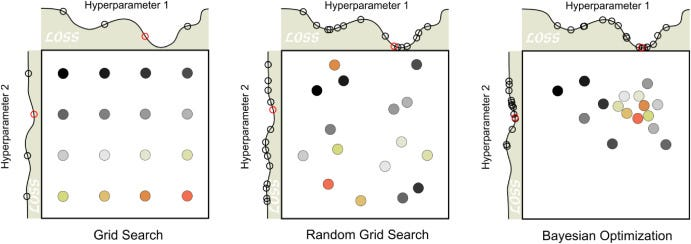
\includegraphics[width=1.0\textwidth]{img/bo.jpg}
		\caption{Confronto tra la ricerca di Grid e Random search con l'ottimizzazione bayesiana.}
	\end{figure}
	\subsection{Spiegazione dell'algoritmo}
	La BO interpreta l’ottimizzazione degli iperparametri come la ricerca del massimo/minimo di una funzione obiettivo costosa ed ignota. Si costruisce un modello surrogato probabilistico (come un Gaussian Process, GP) che stima la funzione obiettivo e quantifica l’incertezza predittiva. Ad ogni iterazione, una funzione di acquisizione determina il prossimo punto da valutare.
	
	\subsubsection{Modello surrogato: Gaussian Process (GP)}
	Un GP definisce, per ogni punto $\lambda$, una distribuzione normale per il valore $f(\lambda)$ con media $\mu(\lambda)$ e varianza $\sigma^2(\lambda)$. Dopo aver osservato alcune valutazioni, si aggiorna $\mu$ e $\sigma$ per riflettere ciò che si è imparato.
	
	\subsubsection{Le fasi del BO}
	
	\begin{enumerate}
		\item \textbf{Campionamento iniziale:} Si comincia con una serie di prove iniziali, selezionando casualmente diverse combinazioni di iperparametri. Per ogni combinazione, si addestra il modello e si calcola una metrica di performance, come la precisione (accuracy) o l'errore quadratico medio (MSE), che funge da risultato della funzione obiettivo.
		\item \textbf{Modello surrogato:} sulla base dei risultati del campionamento iniziale, si costruisce un modello probabilistico, solitamente un Gaussian process, che approssima la funzione obiettivo. Questo modello non solo predice la performance attesa per una data combinazione di iperparametri, ma fornisce anche un'incertezza sulla predizione.
		\item \textbf{Funzione di acquisizione:} viene usata per decidere la prossima combinazione di iperparametri da testare. Questa funzione bilancia l'esplorazione (provare combinazioni di cui si sa poco, per ridurre l'incertezza) e lo sfruttamento (provare combinazioni che il modello surrogato ritiene promettenti, per migliorare la performance).
		\item \textbf{Valutazione della performance:} la nuova combinazione di iperparametri viene utilizzata per addestrare il modello e valutarne le prestazioni. Il risultato di questa valutazione rappresenta il nuovo punto dati che viene aggiunto al nostro set di informazioni.
		\item \textbf{Aggiornamento del modello surrogato:} viene aggiornato con i nuovi risultati. Questo affina le sue predizioni e riduce l'incertezza, permettendo alla funzione di acquisizione di prendere decisioni più informate nelle iterazioni successive.
		\item \textbf{Ripetizione:} i passaggi 3, 4 e 5 vengono ripetuti. Il ciclo si ferma quando si raggiunge un criterio predefinito, come un budget di tempo, un numero massimo di iterazioni, o quando la performance del modello smette di migliorare significativamente.
	\end{enumerate}
	
	\subsection{Vantaggi}
	La Bayesian optimization è un metodo molto \textbf{efficiente}, riducendo drasticamente il numero di valutazioni necessarie, il che la rende ideale per funzioni costose. La sua funzione di acquisizione permette un eccellente \textbf{bilanciamento tra exploration ed exploitation}, permettendo di esplorare nuove regioni e raffinare quelle già note. Inoltre, il modello surrogato offre una \textbf{modellazione dell'incertezza}, che indirizza la ricerca nelle zone potenzialmente più promettenti.
	
	\subsection{Limiti}
	Tra i limiti della BO, si include l'\textbf{overhead computazionale} dovuto al mantenimento e all'aggiornamento del modello surrogato. La sua natura sequenziale rende più \textbf{complessa la parallelizzazione} rispetto a Random o Grid Search. Infine, la sua \textbf{scalabilità è limitata}: pur essendo efficiente su spazi continui di media dimensione, l'ottimizzazione può diventare difficoltosa su spazi molto ampi.
	
	\section{Genetic algorithm (GA)}
	\begin{figure}[H]
		\centering
		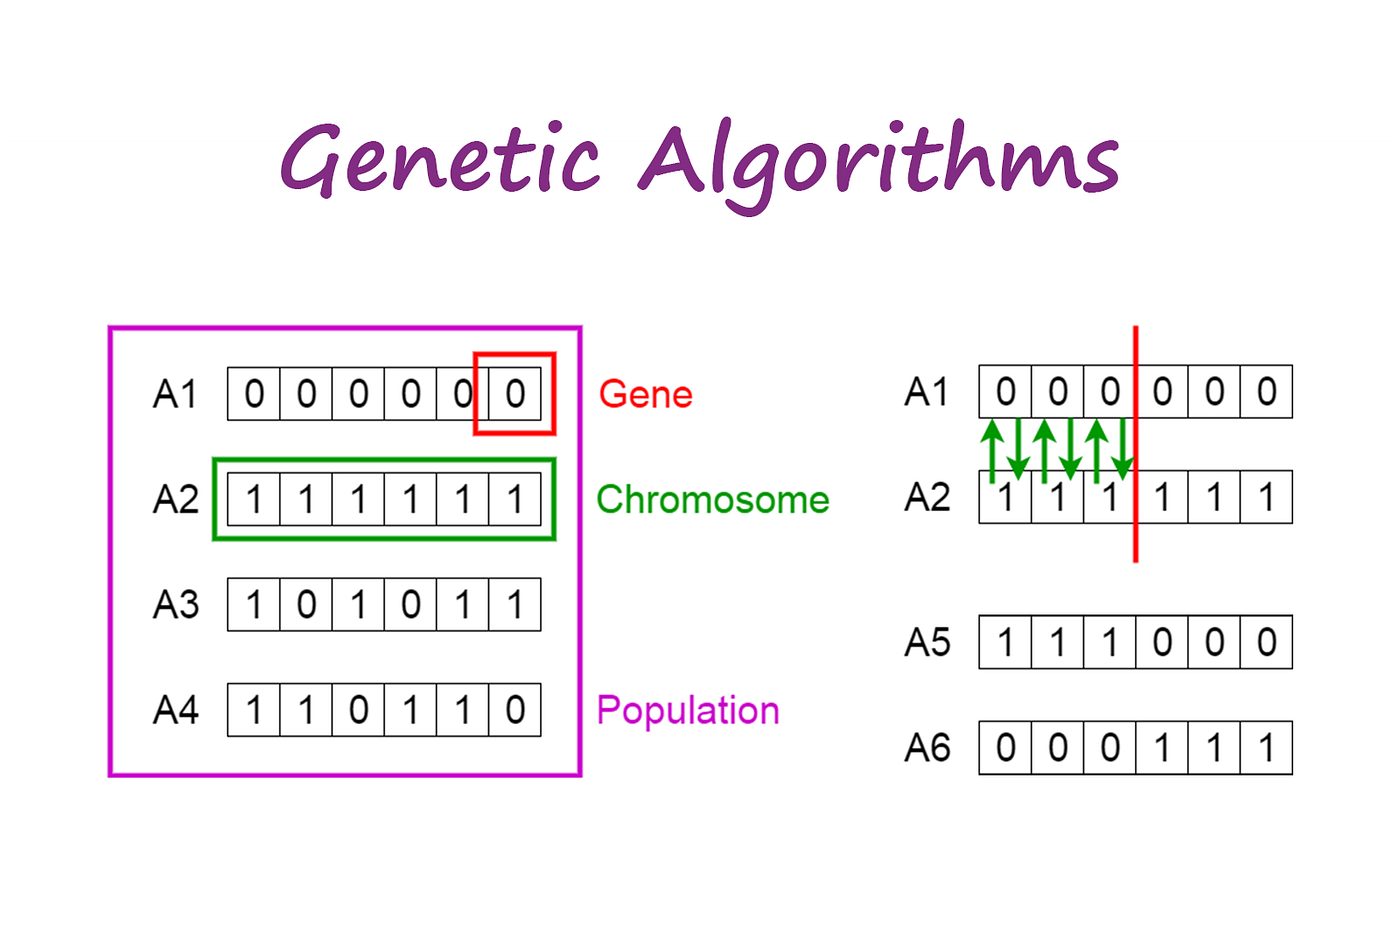
\includegraphics[width=1.0\textwidth]{img/ga.png}
		\caption{Definizione dei concetti principali alla base del funzionamento degli Algoritmi genetici.}
	\end{figure}
	\subsection{Spiegazione dell'algoritmo}
    I Genetic algorithm(GA) sono metodi di ottimizzazione degli iperparametri, ispirati al processo di selezione naturale. Funzionano mantenendo una popolazione di soluzioni e migliorandole nel tempo tramite un processo iterativo. Ad ogni iterazione, detta anche generazione, vengono applicati tre operatori evolutivi principali:
	
	\begin{itemize}
		\item \textbf{Selezione:} gli individui con un punteggio di fitness più alto (le soluzioni "migliori" o più "adatte") vengono scelti per la riproduzione. Questo processo assicura che le caratteristiche positive si diffondano nella popolazione.
		\item \textbf{Crossover:} le soluzioni selezionate vengono combinate per creare nuovi individui "figli". Questo operatore permette di esplorare nuove combinazioni e di mescolare le caratteristiche delle soluzioni migliori.
		\item \textbf{Mutazione:} vengono introdotte piccole, casuali variazioni nelle nuove soluzioni. La mutazione è fondamentale per mantenere la diversità genetica e per evitare che l'algoritmo rimanga bloccato in un'unica soluzione.
	\end{itemize}
	Questi operatori permettono, agli algoritmi genetici, di esplorare un vasto spazio di soluzioni (esplorazione globale) ed, allo stesso tempo, di migliorare le soluzioni promettenti (esplorazione locale), migliorandole sempre di più nel corso delle generazioni.
	
	\subsubsection{Le fasi del GA}
	\begin{figure}[H]
		\centering
		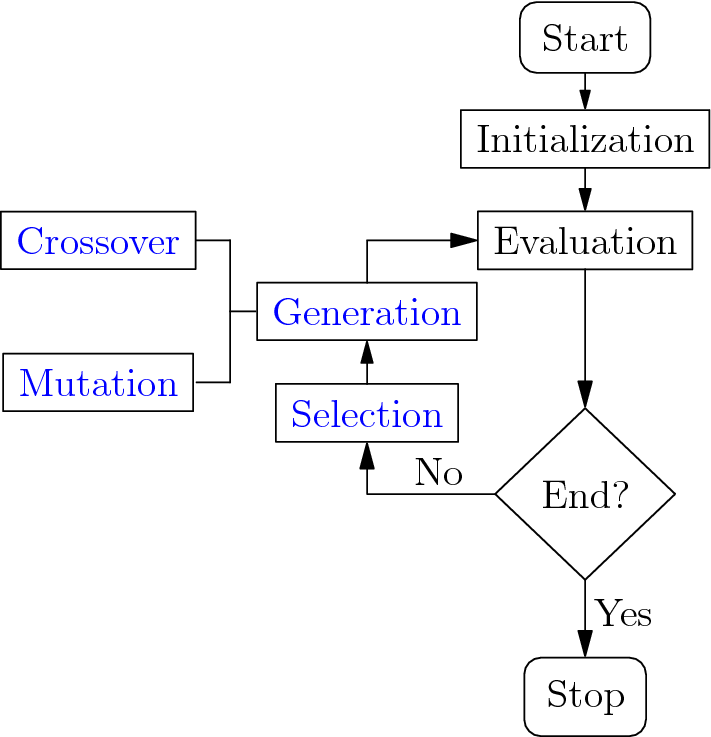
\includegraphics[width=0.5\textwidth]{img/ga_process.png}
		\caption{Le varie fasi del processo del Genetic algorithm.}
	\end{figure}
	\begin{itemize}
		\item \textbf{Inizializzazione:}
		\begin{itemize}
			\item Definire lo spazio di ricerca degli iperparametri.
			\item Generare una popolazione iniziale di $N$ individui casuali.
			\item Impostare i parametri: dimensione popolazione ($N$), generazioni massime ($G_{max}$), tassi di crossover ($p_c$) e mutazione ($p_m$).
		\end{itemize}
		
		\item \textbf{Ciclo evolutivo} (per ogni generazione $g = 1, 2, \ldots, G_{max}$):
		\begin{itemize}
			\item \textbf{Valutazione:} allenare il modello per ogni individuo e calcolare il fitness $f(x_i)$.
			\item \textbf{Selezione:} scegliere i genitori migliori.
			\item \textbf{Crossover:} combinare coppie di genitori con probabilità $p_c$ per generare figli.
			\item \textbf{Mutazione:} introdurre variazioni casuali nei figli con probabilità $p_m$.
			\item \textbf{Sostituzione:} formare la nuova popolazione (strategia elitista o generazionale).
		\end{itemize}
		
		\item \textbf{Terminazione:}
		\begin{itemize}
			\item Fermarsi quando: raggiunto $G_{max}$, nessun miglioramento per $k$ generazioni, o fitness target raggiunto.
			\item Restituire l'individuo con il miglior fitness come soluzione ottimale.
		\end{itemize}
	\end{itemize}
	
	\subsection{Vantaggi}
	Gli algoritmi genetici offrono una \textbf{esplorazione robusta} grazie a crossover e mutazioni, il che li rende adatti a spazi complessi e non lineari per trovare ottimi globali. Sono inoltre efficaci nella \textbf{gestione di spazi misti}, lavorando bene con iperparametri discreti, continui e categorici. Un altro vantaggio è la loro \textbf{parallelizzazione}, in quanto le valutazioni del fitness possono essere distribuite in parallelo.
	
	\subsection{Limiti}
	Tra gli svantaggi, si evidenzia il \textbf{costo computazionale elevato}, poiché richiedono molte generazioni e valutazioni. I risultati dipendono anche da \textbf{iperparametri evolutivi}, come la dimensione della popolazione e i tassi di mutazione/crossover, che devono essere a loro volta ottimizzati. Infine, non c'è una \textbf{garanzia di convergenza} all'ottimo globale, dato che l'algoritmo potrebbe bloccarsi in minimi sub-ottimali se la diversità non viene mantenuta.
	
	\section{Confronto pratico}
	
	\subsection{Criteri per la scelta}
	Nella scelta del metodo di ottimizzazione degli iperparametri, è fondamentale valutare diversi criteri per identificare la soluzione più adatta ad un problema specifico. I criteri principali includono \textbf{l'efficienza}, che si riferisce al numero di valutazioni necessarie per trovare una buona soluzione; \textbf{la scalabilità}, ovvero il comportamento dell'algoritmo all'aumentare della dimensionalità degli iperparametri; \textbf{il supporto per vari tipi di variabili}, che possono essere continue, discrete o categoriche; \textbf{la parallelizzazione}, ovvero la facilità con cui l'algoritmo può essere eseguito su cluster o GPU; \textbf{la robustezza}, ovvero la capacità di gestire rumore e funzioni complesse; e infine \textbf{le risorse computazionali richieste}, che considerano l'overhead e i costi aggiuntivi dell'algoritmo.
	
	\subsection{Tabella riassuntiva comparativa}
	\begin{table}[H]
		\centering
		\small
		\begin{tabular}{lccccc}
			\toprule
			\textbf{Metodo} & \textbf{Efficienza} & \textbf{Scalabilità} & \textbf{Parallelizz.} & \textbf{Complessità} & \textbf{Spazi misti}\\
			\midrule
			Grid search & Bassa & Pessima & Eccellente & Bassa & Bassa\\
			Random search & Media & Buona & Eccellente & Bassa & Bassa\\
			Bayesian opt. & Alta & Limitata & Moderata & Alta & Media\\
			Genetic alg. & Variabile\textsuperscript{*} & Discreta & Eccellente & Media-Alta & Alta\\
			\bottomrule
		\end{tabular}
	\end{table}
	\textsuperscript{*} può essere molto efficace su spazi complessi/discreti, ma richiede molte valutazioni rispetto a BO in spazi piccoli; meno efficiente se valutazioni sono molto care.
	
	\subsection{Matrice decisionale per la scelta del metodo}
	\begin{table}[H]
		\centering
		\footnotesize
		\begin{tabular}{lccc}
			\toprule
			\textbf{Condizioni} & \textbf{Metodo consigliato} & \textbf{Alternativa} & \textbf{Da evitare}\\
			\midrule
			Spazi piccoli (2-3 param.) & Grid Search & Random Search & Bayesian Opt.\\
			Spazi medi/ampi ($>4$ param.) & Random Search & Bayesian Opt. & Grid Search\\
			Valutazioni costose, budget limitato & Bayesian Opt. & Random Search & Grid Search\\
			Spazi molto complessi & Genetic Algorithms & Bayesian Opt. & Grid Search\\
			Multi-obiettivo & Genetic Algorithms & - & Grid/Random Search\\
			Risorse limitate & Random Search & Bayesian Opt. & Grid Search\\
			\bottomrule
		\end{tabular}
	\end{table}
	
	\subsection{Scelta per i casi studio: Random search}
	
	\subsubsection{Motivazioni della scelta}
	Per i casi studio, si è scelto di adottare il Random Search per diverse ragioni. Questo approccio garantisce una notevole \textbf{efficienza su spazi ampi}, offrendo prestazioni superiori al Grid Search quando l'impatto di alcuni iperparametri è marginale. Inoltre, la sua \textbf{scalabilità} lo rende immune all'aumento esponenziale della complessità, mantenendo performance elevate anche con un gran numero di iperparametri. A livello implementativo, la sua \textbf{semplicità} lo rende un metodo ideale per l'implementazione e la parallelizzazione, riducendo la complessità del codice e facilitando l'esecuzione su cluster e GPU. Un'altra motivazione importante è la sua \textbf{flessibilità operativa}, che permette interruzioni anticipate tramite Early stopping ed un facile riutilizzo dei risultati per analisi successive. Infine, il Random Search offre \textbf{il miglior rapporto costo-beneficio}, bilanciando efficienza esplorativa e semplicità computazionale, rendendolo la scelta ideale per il contesto di questa tesi.
	
	\subsection{Ottimizzazione del numero di iterazioni nel Random search}
	Per massimizzare l'efficienza del Random search, è fondamentale stimare il numero minimo di iterazioni necessarie per garantire un'alta probabilità di trovare configurazioni quasi-ottimali. Questo approccio consente di bilanciare l'efficacia esplorativa con il costo computazionale, evitando valutazioni superflue.
	
	\subsubsection{Derivazione teorica della formula}
	La stima del numero di iterazioni richieste si basa sulla teoria della probabilità discreta. Il processo di derivazione segue una logica chiara, partendo dalla probabilità di fallimento in un singolo tentativo. Se in uno spazio di ricerca con $M$ configurazioni totali ne esistono $k$ che consideriamo "quasi-ottimali", la probabilità di non selezionarne una in un singolo campionamento casuale è:
	$$P(\text{fallimento singolo}) = 1 - \frac{k}{M}$$
	La probabilità di fallire in tutti gli $n$ tentativi indipendenti è quindi:
	$$P(\text{fallimento totale}) = \left(1 - \frac{k}{M}\right)^n$$
	Da qui, si ricava la probabilità di successo, ovvero di trovare almeno una configurazione top-$k$ in $n$ tentativi:
	$$P(\text{successo}) = 1 - \left(1 - \frac{k}{M}\right)^n$$
	Infine, per determinare il numero di iterazioni $n$ necessarie per raggiungere una probabilità di successo $P$ desiderata, si risolve la formula per $n$:
	$$1 - \left(1 - \frac{k}{M} \right)^n = P \quad \Longrightarrow \quad n = \frac{\ln(1 - P)}{\ln\left(1 - \frac{k}{M} \right)}$$
	Quando il numero delle migliori configurazioni ($k$) è molto più piccolo del numero totale di configurazioni ($M$), si può usare l'approssimazione $\ln(1 - x) \approx -x$ per $x$ piccolo. In questo caso, la formula si semplifica in:
	$$n \approx - \frac{\ln(1 - P)}{k/M}$$
	
	\subsubsection{Vantaggi dell'approccio probabilistico}
	L'approccio probabilistico al Random search offre notevoli vantaggi. Garantisce un'elevata \textbf{efficienza computazionale}, riducendo drasticamente il numero di valutazioni necessarie. Fornisce inoltre un forte \textbf{controllo statistico}, offrendo una garanzia probabilistica di trovare soluzioni quasi-ottimali. Grazie alla sua \textbf{flessibilità}, permette di modulare il trade-off tra accuratezza desiderata ($P$) e il costo computazionale ($n$). Infine, il metodo si distingue per la sua \textbf{scalabilità}, adattandosi automaticamente alla dimensione dello spazio di ricerca, un aspetto cruciale in contesti con molti iperparametri.
	
	\chapter{Studio di ablazione e Pruning post-training}
	
	\section{Introduzione}
	Questo capitolo introduce e analizza due metodologie fondamentali per l'ottimizzazione e la comprensione dei modelli di Machine e Deep Learning: lo studio di ablazione ed il post-training pruning. L'obiettivo è esplorare come queste tecniche permettano non solo di diagnosticare il funzionamento interno di un modello, ma anche di migliorarne l'efficienza senza comprometterne significativamente le prestazioni. Il testo inizia descrivendo la natura degli studi di ablazione e la loro utilità nell'identificare le componenti critiche di un modello. Successivamente, il capitolo si concentra sul pruning post-training, partendo da una definizione generale per poi focalizzarsi sulla tecnica di L1 pruning applicata a diverse architetture, come i classici MLP e le KAN. Infine, viene fornito un confronto tra il pruning rank-based per le Random Forest e il cumulative pruning per XGBoost, illustrando come queste tecniche possano essere adattate per ottimizzare diversi tipi di ensemble. Per la sua efficienza e la sua flessibilità, il pruning L1 è stato scelto come tecnica di riferimento per l'ottimizzazione dei modelli di deep learning presentati in questa ricerca. \cite{meyes2019ablation, vadera2021dnnpruning, tsoumakas1970rfpruning}
	
	\section{Studi di ablazione}
	Gli studi di ablazione rappresentano una metodologia fondamentale nell'analisi e nell'ottimizzazione dei modelli di machine e deep learning, che consiste nella rimozione temporanea di una componente del modello, come un layer o gruppo di parametri, per osservare l'impatto sulle prestazioni. Si tratta di un esperimento diagnostico che aiuta a comprendere quali elementi contribuiscono maggiormente alla capacità predittiva del modello. In questo contesto, il pruning post-training viene utilizzato come una tecnica complementare che permette non solo di comprendere l'importanza delle componenti del modello, ma anche di ottenere versioni più efficienti senza compromettere significativamente le prestazioni.
	
	\subsection{Definizione}
	Per formalizzare matematicamente il concetto di ablazione, consideriamo un modello $f_\theta$ dove $\theta$ rappresenta l'insieme completo dei suoi parametri, e $L(\theta)$ indica la funzione di perdita del modello. Dato un sottoinsieme specifico di parametri $S$, la variazione di performance dovuta all'ablazione può essere quantificata come:
	
	\[
	\Delta_S = L(\theta_{-S}) - L(\theta)
	\]
	
	In questa formulazione, $\theta_{-S}$ rappresenta il modello con la componente $S$ rimossa. Un valore elevato di $\Delta_S$ indica che la componente $S$ fornisce un contributo importante alle prestazioni del modello. Questa definizione matematica fornisce una base quantitativa per valutare l'importanza relativa delle diverse componenti del modello.
	
	\subsection{Benefici}
	Gli studi di ablazione offrono diversi benefici significativi. Innanzitutto, permettono l'\textbf{identificazione delle componenti critiche}, aiutando a comprendere la sensibilità del modello a specifiche parti della sua architettura e rivelando potenziali vulnerabilità o punti di forza. Inoltre, i risultati di questi studi fungono da \textbf{guida per la semplificazione} del modello, fornendo una base empirica per le decisioni di pruning. Infine, l'analisi di come la rimozione di una componente specifica influenzi le previsioni facilita l'\textbf{interpretazione del comportamento del modello}, contribuendo a una maggiore comprensione dei meccanismi interni che portano alle predizioni finali.
	
	\section{Pruning post-training}
	
	\subsection{Definizione}
	Il pruning post-training può essere considerato come l'applicazione di un operatore $\mathcal{P}$ ad un modello già addestrato, che elimina parametri secondo criteri specifici (come l'ampiezza del parametro, l'importanza stimata, o il contributo marginale) per avere un modello più leggero. \\
	La scelta del criterio di pruning influenza significativamente sia l'efficacia della compressione sia il mantenimento delle prestazioni. I criteri più comuni includono la magnitudine dei parametri, misure di sensibilità basate sui gradienti, e metriche di importanza derivate dall'analisi della struttura del modello.
	
	\subsection{Benefici}
	I benefici del pruning sono molteplici. Il primo e più evidente è la \textbf{riduzione della memoria e del tempo di inferenza}: il pruning riduce lo spazio di memoria richiesto e il tempo necessario per le predizioni, aspetti critici per il deployment in ambienti con risorse limitate. L'obiettivo primario è il \textbf{mantenimento delle prestazioni}, bilanciando l'efficienza e l'accuratezza del modello in modo che le performance rimangano entro una tolleranza accettabile. Infine, riducendo il numero di elementi attivi, il pruning contribuisce a un aumento dell'\textbf{interpretabilità}, facilitando l'analisi e la comprensione del contributo delle parti rimanenti.
	
	\subsection{Trade-off bias-varianza}
	La riduzione della complessità del modello, attraverso l'eliminazione di parametri, tende a diminuire la varianza, riducendo il rischio di overfitting sui dati di training. Tuttavia, questa semplificazione può introdurre bias, limitando la capacità del modello di catturare pattern complessi nei dati. L'obiettivo pratico del pruning consiste nel trovare il punto ottimale dove la riduzione della varianza compensa l'aumento del bias, mantenendo prestazioni globalmente superiori. Questo equilibrio è altamente dipendente dalla natura dei dati, dalla complessità del task, e dalle caratteristiche specifiche dell'architettura del modello.
	
	\section{Pruning L1 post-training per MLP e KAN}
	
	\subsection{Definizione}
	Dato un insieme di parametri del modello $\Theta = \{\theta_1, \theta_2, \dots, \theta_N\}$, la procedura di L1 pruning opera applicando una trasformazione a ciascun parametro $\theta_i$, che è definita da una soglia di potatura $\lambda$, che viene tipicamente determinata a livello globale per il modello o a livello locale per ciascun strato.
	
	La formula è:
	$$
	\theta_i^{\text{pruned}} = \begin{cases}
		0 & \text{se } |\theta_i| \le \lambda \\
		\theta_i & \text{se } |\theta_i| > \lambda
	\end{cases}
	$$
	In questa formulazione, se la magnitudine assoluta ($|\theta_i|$) di un parametro è inferiore o uguale alla soglia $\lambda$, esso viene permanentemente impostato a zero. Al contrario, se la sua magnitudine è superiore a $\lambda$, il parametro viene mantenuto invariato.
	
	\subsection{Considerazioni specifiche per le KAN}
	L'applicazione del L1 pruning alle KAN é abbastanza diverso rispetto a MLP. La motivazione principale risiede nella diversa natura dei parametri che compongono questi modelli. Nelle MLP, i parametri sono pesi e bias che operano su connessioni lineari, mentre nelle KAN sono coefficienti che definiscono funzioni univariate (tipicamente B-spline) su ogni arco della rete. \\
	Il pruning su KAN può essere implementato in due modi. Il primo approccio prevede la rimozione di coefficienti locali delle spline, riducendo la risoluzione locale della rappresentazione funzionale mantenendo la struttura generale. Il secondo approccio elimina intere funzioni su specifici archi della rete, semplificando direttamente l'architettura della KAN. \\
	La scelta tra questi approcci deve considerare l'impatto sulla continuità delle funzioni e sulla loro interpretabilità. La rimozione di coefficienti locali mantiene la struttura generale ma può creare delle discontinuità o irregolarità indesiderate nella curva che la spline rappresenta, mentre l'eliminazione di intere funzioni preserva la continuità locale ma può alterare significativamente la capacità espressiva del modello.
	
	\section{Pruning per Ensemble: Rank-based pruning per Random forest}
	
	\subsection{Principio fondamentale}
	Il rank-based pruning per Random forest si basa sul principio che non tutti gli alberi nell'ensemble contribuiscono equamente alle prestazioni finali. Alcuni alberi possono essere ridondanti o addirittura dannosi per la capacità di generalizzazione dell'ensemble, rendendo la loro rimozione vantaggiosa sia in termini di efficienza e prestazioni. L'approccio implementato definisce per ogni albero $m$ un contributo stimato alle prestazioni, quantificato attraverso la variazione di errore $\Delta L_m$ che si osserverebbe rimuovendo l'albero dall'ensemble. Gli alberi con contributo minore sono candidati prioritari per la rimozione durante il processo di pruning.
	
	\subsection{Criterio di ranking basato sulla feature importance}
	Invece di valutare l'impatto della rimozione di ogni singolo albero sull'errore complessivo, il criterio di ranking si basa sulle feature importance di ogni singolo albero. Specificamente, l'importanza di un albero $m$ viene calcolata come la somma delle feature importance che l'albero utilizza. La logica sottostante è che un albero che si basa su feature più discriminative, che riducono significativamente l'entropia o l'indice di Gini, è probabile che fornisca un contributo maggiore all'ensemble. Questo metodo offre un vantaggio computazionale significativo rispetto a un'analisi diretta dell'errore.
	
	\subsection{Procedura di selezione}
	La procedura di selezione implementa una strategia greedy che ordina gli alberi per importanza decrescente e seleziona i primi $k$ alberi, dove $k$ è determinato dal pruning ratio desiderato. Questa scelta greedy è giustificata dall'assunzione che l'utilità marginale degli alberi decresce monotonicamente con il loro ranking. La validazione empirica di questa assunzione rappresenta un aspetto critico della metodologia, poiché la submodularità della funzione di utilità non è sempre garantita negli ensemble reali. L'implementazione, infatti, include procedure di validazione che verificano che la selezione greedy produca risultati coerenti.
	
	\section{Pruning per Ensemble: Cumulative pruning per XGBoost}
	
	\subsection{Criterio di pruning cumulativo}
	Il pruning cumulativo implementato si basa su un principio di selezione basato sull'ordine: vengono mantenuti solo i primi $n$ round di boosting, scartando i successivi. Il presupposto è che le prime iterazioni, che hanno l'obiettivo di ridurre al massimo l'errore iniziale, contribuiscano in modo più significativo e non siano ridondanti come gli alberi meno performanti che si trovano alla fine del processo di training. La percentuale di iterazioni da mantenere è controllata direttamente dal pruning ratio, che determina la frazione di modello da eliminare. In pratica, l'algoritmo mantiene le iterazioni da $1$ a $n$, dove $n$ è calcolato come $(1 - \text{pruning ratio})$ moltiplicato per il numero totale di round di boosting.
	
	\subsection{Procedura di selezione}
	A differenza di Random forest, che può semplicemente rimuovere alberi dalla lista degli "estimators", XGBoost richiede un'operazione più delicata a causa della natura additiva delle sue predizioni.
	
	Il processo tecnico consiste in:
	\begin{enumerate}
		\item \textbf{Calcolo del numero di iterazioni da mantenere:} si determina il numero di alberi da utilizzare per la predizione. Questo valore viene calcolato in base ad un pruning ratio definito. Nei problemi di classificazione multiclasse, ogni round di boosting aggiunge un albero per ogni classe.
		\item \textbf{Predizione con iterazioni limitate:} invece di modificare la struttura del modello, si sfrutta una funzionalità di XGBoost che permette di specificare il numero di alberi da usare per la predizione. Il modello addestrato mantiene al suo interno tutti gli alberi, ma per calcolare il risultato finale si usa solo l'insieme limitato di alberi specificato.
	\end{enumerate}
	
	Se l'obiettivo è creare un modello più leggero da salvare o esportare, è possibile potare il modello in modo permanente. Questo si ottiene limitando l'ensemble agli alberi selezionati e salvando il nuovo modello ridotto. Questo processo è utile per ridurre l'occupazione di memoria e rendere il modello più efficiente per la distribuzione in produzione, una volta che la migliore configurazione è stata identificata tramite lo studio di ablazione.
	
	\chapter{Casi di studio}
	
	\section{Progettazione dei casi di studio}
	
	\subsection{Tecnologie e librerie}
	Il workflow sperimentale e di analisi è stato interamente sviluppato in \texttt{Python}, con un insieme di librerie comuni ai tre casi studio e componenti specifiche in base alla natura del problema affrontato. \\
	Per la manipolazione dei dati si è fatto uso di \textbf{NumPy} e \textbf{pandas}, mentre la visualizzazione è stata realizzata con \textbf{matplotlib} e \textbf{seaborn} (con configurazione \texttt{sns.set\_theme()}). I moduli \texttt{json}, \texttt{os}, \texttt{inspect} e \texttt{copy} sono stati utilizzati per la gestione dei metadati, il salvataggio dei risultati e la serializzazione delle configurazioni. \\
	Le reti neurali (MLP, KAN e loro estensioni CNN nel terzo caso studio) sono state implementate in \textbf{PyTorch}, facendo ricorso a \texttt{torch.nn}, \texttt{torch.optim}, \texttt{torch.utils.data} e \texttt{torch.nn.utils.prune}, con funzioni di supporto definite in \texttt{torch.nn.functional}. Nel terzo caso studio è stato inoltre utilizzato \textbf{torchvision} per le trasformazioni e la gestione delle immagini. La libreria \textbf{kan} è stata integrata in tutti i casi studio per l’implementazione della Kolmogorov-Arnold Network.
	Per gli approcci ensemble, sono stati adottati \textbf{scikit-learn} (RandomForestRegressor, RandomForestClassifier, metriche di regressione e classificazione, pipeline, \texttt{ColumnTransformer}, scaling, encoding, \texttt{ParameterSampler}, \texttt{KFold}, \texttt{RandomizedSearchCV}, \texttt{TimeSeriesSplit}) e \textbf{XGBoost}. Nel secondo e terzo caso studio si è inoltre fatto uso di \textbf{imblearn} (\texttt{SMOTE}, \texttt{ImbPipeline}) per il bilanciamento delle classi. \\
	Gli strumenti ausiliari hanno incluso \texttt{tqdm} per le progress bar (caso studio 3), \texttt{logging} per il tracciamento degli esperimenti e librerie standard come \texttt{random}, \texttt{time}, \texttt{glob}, \texttt{zipfile}, \texttt{pathlib} e \texttt{PIL.Image} per la gestione dei dataset e delle immagini.
	
	\subsection{Ambienti di sviluppo e infrastruttura}
	La prototipazione ed il debug sono stati effettuati su \textbf{Google Colab}, sfruttando notebook interattivi; le sperimentazioni su larga scala e l’addestramento intensivo dei modelli sono stati condotti sul \textbf{Cluster HPC} dell’Università di Bologna, con allocazione di GPU tramite SLURM. \\
	Per la riproducibilità delle dipendenze, sono stati creati ambienti virtuali dedicati (\texttt{venv}) e un file \texttt{requirements.txt}. I risultati di ogni run, insieme a configurazioni ed iperparametri, sono stati serializzati in \texttt{JSON}, mentre i notebook eseguiti sul cluster sono stati automaticamente convertiti in HTML per la documentazione.
	
	\subsection{Linguaggi, scripting e automazione del workflow}
	Il linguaggio principale è \texttt{Python}. Le analisi esplorative e la reportistica sono state realizzate in Jupyter notebooks, mentre l’automazione degli esperimenti e la sottomissione su cluster sono state gestite tramite script \texttt{bash} integrati con SLURM. \\
	La conversione automatica ed esecuzione dei notebook è stata gestita con \texttt{nbconvert}, così da produrre sia versioni aggiornate in formato notebook che report in HTML. Ogni esperimento ha registrato seed, configurazioni ed eventi salienti del training con logging strutturato, assicurando piena riproducibilità.
	
	\subsection{Script di sottomissione (Cluster GPU)}
	La struttura degli script SLURM è risultata uniforme tra i casi studio, con differenze solo nelle risorse richieste, nel nome del job e nel notebook eseguito. Un esempio generico è riportato di seguito:
	
	\begin{verbatim}
		#!/bin/bash
		#SBATCH --job-name=Generic_Case
		#SBATCH --mail-type=ALL
		#SBATCH --mail-user=martin.tomassi@studio.unibo.it
		#SBATCH --time=120:00:00
		#SBATCH --nodes=1
		#SBATCH --ntasks-per-node=1
		#SBATCH --cpus-per-task=8
		#SBATCH --mem=60G
		#SBATCH --partition=l40
		#SBATCH --output=output_jupyter_exec_job_%j.txt
		#SBATCH --chdir=/scratch.hpc/martin.tomassi
		#SBATCH --gres=gpu:1
		
		export JUPYTER_CONFIG_DIR=
				"/scratch.hpc/martin.tomassi/jupyter_config_$SLURM_JOB_ID"
		export MPLCONFIGDIR=
				"/scratch.hpc/martin.tomassi/matplotlib_cache_$SLURM_JOB_ID"
		mkdir -p "$JUPYTER_CONFIG_DIR"
		mkdir -p "$MPLCONFIGDIR"
		
		source venv_case/bin/activate
		jupyter nbconvert --to notebook
				--execute case_notebook.ipynb
				--output case_notebook_trained.ipynb
		jupyter nbconvert --to html case_notebook_trained.ipynb
		deactivate
		
		rm -rf "$JUPYTER_CONFIG_DIR"
		rm -rf "$MPLCONFIGDIR"
	\end{verbatim}
	
	\subsection{Scelte architetturali ed iperparametri}
	Le scelte architetturali e gli iperparametri finali sono stati specifici per ciascun caso studio. Le configurazioni dettagliate, incluse nelle tabelle dei singoli capitoli, documentano gli iperparametri selezionati dopo la fase di ottimizzazione. In tutti i casi, si è fatto ricorso a \textit{Early stopping} per migliorare la generalizzazione.
	
	\section{Addestramento dei modelli}
	
	In tutti i casi studio considerati (regressione CO2, classificazione PM2.5, classificazione età da immagini) è stata adottata una pipeline di addestramento omogenea che mira a garantire comparabilità sperimentale tra le architetture (MLP, KAN, Random Forest, XGBoost).
	
	\subsection{Pipeline di preprocessing}
	Le trasformazioni iniziali applicate alle variabili indipendenti sono state incapsulate in pipeline riutilizzabili (ad es. \texttt{ColumnTransformer}) per evitare data leakage e garantire riproducibilità. La selezione delle feature ha rimosso colonne non informative o ridondanti; le variabili categoriche sono state codificate con \texttt{OneHotEncoder} eseguito all'interno della pipeline; le feature numeriche sono state standardizzate tramite \texttt{StandardScaler}. I missing values sono stati trattati in modo coerente tra gli esperimenti: dove possibile si è preferita la rimozione controllata delle righe; si sottolinea che, sebbene XGBoost gestisca NaN nativamente, per confronto omogeneo i NaN sono stati generalmente eliminati. Per i dataset di immagini il preprocessing include resize e crop centrato a $224\times224$, normalizzazione canale-per-canale e data augmentation (flip orizzontale, rotazioni lievi, jitter di luminosità/contrasto) applicata esclusivamente in fase di training. Per problemi di classificazione sbilanciata si è fatto ricorso a tecniche di bilanciamento approcciate esclusivamente sul training fold (SMOTE per dati tabellari, pesi di classe o \texttt{WeightedRandomSampler} per immagini).
	
	\subsection{Suddivisione dei dati e validazione}
	Il dataset è stato suddiviso in test set indipendente (circa 20\%) e training pool (circa 80\%). Per i dataset non temporali si è impiegata una Nested Cross-Validation con outer KFold = 5 e inner KFold = 3 in combinazione con Random Search per la selezione degli iperparametri e la stima della performance generalizzata. Per i dataset temporali si è usata una Time Series Cross Validation che rispetta l'ordine cronologico delle osservazioni.
	
	\subsection{Metriche e intervalli di confidenza}
	Le metriche sono state scelte in funzione del tipo di problema. Per i compiti di regressione, sono state utilizzate:
	\begin{itemize}
		\item \textbf{MSE} (Mean Squared Error): \(\text{MSE} = \frac{1}{n} \sum_{i=1}^{n} (y_i - \hat{y}_i)^2\).
		\item \textbf{MAE} (Mean Absolute Error): \(\text{MAE} = \frac{1}{n} \sum_{i=1}^{n} |y_i - \hat{y}_i|\).
		\item \textbf{MAPE} (Mean Absolute Percentage Error): \(\text{MAPE} = \frac{100}{n} \sum_{i=1}^{n} \left| \frac{y_i - \hat{y}_i}{y_i} \right|\), calcolata escludendo i casi con \(y_i=0\) o valori non finiti.
		\item \textbf{R\(^2\)} e \textbf{R\(^2\)-adjusted}:
		\[
		R^2 = 1 - \frac{\sum (y_i - \hat{y}_i)^2}{\sum (y_i - \bar{y})^2}, \qquad
		R^2_{adj} = 1 - (1 - R^2)\frac{n-1}{n-k-1},
		\]
		dove \(n\) è il numero di osservazioni e \(k\) il numero di predittori.
		\item \textbf{Max Error}: \(\max_i |y_i - \hat{y}_i|\).
	\end{itemize}
	
	Per i compiti di classificazione, sono state considerate:
	\begin{itemize}
		\item \textbf{Accuracy}:
		\[
		\text{Accuracy} = \frac{\text{Numero di predizioni corrette}}{\text{Numero totale di predizioni}} = \frac{\sum_{i=1}^{N} \mathbb{I}(y_i = \hat{y}_i)}{N}
		\]
		dove $y_i$ è il valore vero, $\hat{y}_i$ è il valore predetto e $\mathbb{I}(\cdot)$ è la funzione indicatrice.
		
		\item \textbf{Precisione} ($P$) e \textbf{Recall} ($R$):
		\[
		P = \frac{\text{TP}}{\text{TP} + \text{FP}}, \quad R = \frac{\text{TP}}{\text{TP} + \text{FN}}
		\]
		dove TP = True Positives, FP = False Positives, FN = False Negatives.
		
		\item \textbf{F1-score}: basato su Precisione e Recall della classe specifica.
		\[
		F1 = 2 \cdot \frac{P \cdot R}{P + R}
		\]
		
		\item \textbf{F1-score macro e weighted}:
		\[
		F1_{\text{macro}} = \frac{1}{C} \sum_{c=1}^{C} F1_c
		\]
		\[
		F1_{\text{weighted}} = \sum_{c=1}^{C} F1_c \cdot \frac{N_c}{N}
		\]
		dove $C$ è il numero di classi, $F1_c$ è l'F1-score della classe $c$, $N_c$ è il numero di istanze della classe $c$, e $N$ è il numero totale di istanze.
		
		\item \textbf{Confusion Matrix}: la matrice di confusione è una tabella che riassume la performance di un modello di classificazione. Per un problema di classificazione binaria, la sua struttura è:
		\[
		\begin{array}{c|c|c|}
			\multicolumn{1}{c}{} & \multicolumn{2}{c}{\textbf{Predetto}} \\
			\cline{2-3}
			\multicolumn{1}{c}{\textbf{Reale}} & \text{Positivo} & \text{Negativo} \\
			\cline{2-3}
			\text{Positivo} & \text{TP} & \text{FN} \\
			\cline{2-3}
			\text{Negativo} & \text{FP} & \text{TN} \\
			\cline{2-3}
		\end{array}
		\]
		dove TP = True Positives, FP = False Positives, FN = False Negatives, TN = True Negatives.
		
		\item \textbf{AUC-ROC weighted}: l'area sotto la curva ROC (Receiver Operating Characteristic), che traccia il True Positive Rate (TPR) contro il False Positive Rate (FPR) per diverse soglie.
		\[
		\text{TPR} = \frac{\text{TP}}{\text{TP} + \text{FN}}, \quad \text{FPR} = \frac{\text{FP}}{\text{FP} + \text{TN}}
		\]
		L'AUC-ROC weighted è la media pesata dell'AUC di ogni classe.
		
		\item \textbf{AUC-PR weighted}: l'area sotto la curva Precision-Recall, che traccia la Precisione in funzione del Recall.
		\[
		\text{AUC-PR} = \int_{0}^{1} \text{Precision}(\text{Recall}) \, d(\text{Recall})
		\]
		L'AUC-PR weighted è la media pesata dell'AUC-PR di ogni classe.
	\end{itemize}
	
	\paragraph{Intervalli di confidenza}  
	Per tutte le metriche principali è stata stimata l’incertezza statistica tramite bootstrap, un metodo di ricampionamento che approssima la distribuzione empirica delle metriche. La procedura consiste nel generare $B$ campioni bootstrap $S_1, S_2, \dots, S_B$ estraendo con ripetizione $N$ elementi dal test set $S$; su ciascun campione viene calcolata la metrica $\text{M}(S_i)$. L’intervallo di confidenza al livello $(1-\alpha)$ si ottiene quindi dai percentili della distribuzione delle metriche:  
	\[
	\text{CI}_{(1-\alpha)} = \left( \text{Percentile}_{\alpha/2}(\text{M}), \; \text{Percentile}_{1-\alpha/2}(\text{M}) \right).
	\]
	Nel presente lavoro sono riportati intervalli al 95\%, calcolati in modo uniforme in tutti i casi studio per le seguenti metriche:
	\begin{itemize}
		\item Regressione: $R^2$, MSE, MAE, MAPE;
		\item Classificazione: Accuracy, F1 macro, F1 weighted, AUC-ROC weighted, AUC-PR weighted.
	\end{itemize}
	
	\paragraph{Complessitá dei modelli}
	Oltre alle metriche predittive, per tutti i casi studio è stata calcolata la complessità dei modelli:
	\begin{itemize}
		\item Per le KAN, la formula per calcolare la sua complessità è:
		\[
		P_{\text{KAN}} = \sum_{i=0}^{L-1} (N_i \cdot N_{i+1}) \cdot (G+k+3) + N_{i+1}
		\]
		dove $L$ è il numero di strati, $N_i$ indica le dimensioni dello strato $i$, $G$ è la dimensione della griglia e $k$ è l'ordine della spline.
		
		\item Per le MLP, la formula è:
		\[
		P_{\text{MLP}} = \sum_{i=1}^{L-1} N_i \cdot N_{i+1} + N_{i+1}
		\]
		
		\item Per Random Forest e XGBoost, la complessità è il numero totale di nodi in tutti gli alberi dell'ensemble.
		\[
		\text{Complessità}_{\text{Albero}} = \sum_{i=1}^{T} \text{Nodi}_i
		\]
		dove $T$ è il numero totale di alberi nell'ensemble e $\text{Nodi}_i$ è il numero di nodi nell'albero $i$.
	\end{itemize}
	
	\chapter{Primo Caso Studio: Regressione su emissioni di automobili}
	
	\section{Introduzione}
	Il presente caso studio affronta la previsione delle emissioni di CO2 di veicoli a partire da caratteristiche tecniche e di consumo (anno di produzione, cilindrata, tipo di trasmissione e carburante, consumo L/100km, ecc.). Il dataset utilizzato deriva dalla fusione di tre sorgenti ufficiali: i dati originali provengono dalla Vehicle Certification Agency (VCA) del Department for Transport del Regno Unito, dal sito ufficiale del Governo canadese e dal Instituto para la Diversificación y Ahorro de la Energía (IDAE), istituzione spagnola; il materiale è stato fornito in forma pre-elaborata da terze parti \cite{olivi2024car}. Per questo motivo, la trattazione qui riportata si concentra sulle fasi di modellazione, validazione ed analisi dei risultati, più che sulle operazioni di preprocessing. Per ottenere stime di performance affidabili si adotta il Nested CV con Random Search per l’ottimizzazione degli iperparametri ed una valutazione che combina indicatori di accuratezza con misure di complessità ed intervalli di confidenza. Inoltre, sono condotti studi di ablazione che valutano l’impatto di tecniche di pruning sui diversi tipi di modello per investigare il trade-off tra compressione e mantenimento della qualità predittiva. \\
	Nel capitolo seguente vengono presentati, in ordine: una sintetica nota sull’origine e lo stato del dataset; la pipeline di preprocessing e le scelte di split; la descrizione delle procedure di training e ottimizzazione; i risultati principali con le valutazioni comparative e gli esperimenti di ablazione con le considerazioni finali sul compromesso performance/complessità.
	
	\section{Data preparation}
	
	\subsection{Riassunto delle principali trasformazioni}
	Le principali trasformazioni applicate includono: l'unione delle tre sorgenti in un unico dataframe coerente; l'omogeneizzazione degli schemi attraverso la mappatura e la ridenominazione delle colonne per ottenere uno schema comune; la pulizia testuale con la standardizzazione e capitalizzazione dei valori e la rimozione di suffissi o annotazioni spurie. Inoltre, è stata effettuata un'imputazione conservativa, utilizzando la mediana (globale o per gruppo/categoria) per riempire i valori mancanti numerici significativi, con eliminazioni conservative per categoria quando necessario. Infine, sono stati applicati dei filtri per eliminare righe prive della variabile target (\texttt{CO2\_Emissions}) o prive di attributi ritenuti fondamentali per l'allenamento dei modelli.
	
	\section{Addestramento dei modelli}
	
	Il dataset finale comprende le seguenti features:
	\begin{itemize}
		\item \texttt{Year}: anno di produzione del veicolo (numerica);
		\item \texttt{Manufacturer}: casa automobilistica (categorica);
		\item \texttt{Model}: nome del modello (categorica);
		\item \texttt{Engine\_cm3}: cilindrata in \(\mathrm{cm^3}\) (numerica);
		\item \texttt{Transmission\_type}: Automatic / Manual (categorica);
		\item \texttt{Fuel\_type}: Petrol / Diesel / LPG / \ldots (categorica);
		\item \texttt{Fuel\_consumption}: L/100km (numerica).
	\end{itemize}
	La variabile target da prevedere è \texttt{CO2\_Emissions} (g/km).
	
	\subsection{Strategia di training comune e griglie di iperparametri}
	La strategia di training è stata omogenea per tutti i modelli considerati. Le procedure comuni adottate sono le seguenti: il protocollo di validazione impiega una Nested CV con un outer KFold $= 5$ e un inner KFold $= 3$. Il ciclo interno esegue una Random Search sulle griglie di iperparametri. La migliore configurazione trovata viene riaddestrata sul sottoinsieme interno e valutata sul corrispondente outer test fold. Per la Random Search, il numero di iterazioni $n$ è stato scelto con una logica probabilistica per assicurare una probabilità del 90\% di includere almeno una delle 10 migliori configurazioni. Per le reti neurali, l'ottimizzazione è stata gestita con l'ottimizzatore \texttt{Adam} e la funzione di perdita \texttt{MSELoss}, con una regolarizzazione L2 opzionale. Le epoche massime sono 1000, ma con l'uso di un Early stopping per interrompere il training in caso di mancato miglioramento. Infine, la \textbf{valutazione finale} di ogni outer fold ha incluso il calcolo delle metriche (MSE, MAE, MAPE, $R^2$, $R^2$-adjusted, Max Error), degli intervalli di confidenza al 95\% per MSE, MAE e MAPE e della complessità del modello. Inoltre, la funzione di attivazione della MLP é la ReLU. \\
	
	Di seguito sono riportate le griglie di iperparametri entro cui la Random Search esplora le combinazioni, al fine di individuare quelle che forniscono i risultati migliori per ciascun modello.
	\smallskip
	\noindent\textbf{MLP} \quad (Random Search: $n=15$)
	\begin{itemize}
		\item \texttt{input\_dim:} dimensionalità input
		\item \texttt{hidden\_sizes:} [(32,32), (64,64), (128,)]
		\item \texttt{dropout:} [0.1, 0.2, 0.5]
		\item \texttt{lr:} [$10^{-3}$, $10^{-4}$]
		\item \texttt{batch\_size:} 32
		\item \texttt{l2\_lambda:} [0, $10^{-5}$, $10^{-4}$, $10^{-3}$]
	\end{itemize}
	
	\smallskip
	\noindent\textbf{KAN} \quad (Random Search: $n=6$)
	\begin{itemize}
		\item \texttt{input\_dim:} dimensionalità input
		\item \texttt{width:} [(8,4), (16,8)]
		\item \texttt{grid:} [5, 10]
		\item \texttt{k:} [2, 4]
		\item \texttt{seed:} 0
		\item \texttt{lr:} $10^{-3}$
		\item \texttt{batch\_size:} 32
		\item \texttt{l2\_lambda:} [0, $10^{-5}$, $10^{-4}$, $10^{-3}$]
	\end{itemize}
	
	\smallskip
	\noindent\textbf{Random Forest} \quad (Random Search: $n=32$)
	\begin{itemize}
		\item \texttt{n\_estimators:} [100, 200, 300, 500]
		\item \texttt{max\_depth:} [10, 20, 30]
		\item \texttt{min\_samples\_split:} [10, 20, 30]
		\item \texttt{min\_samples\_leaf:} [5, 10]
		\item \texttt{max\_features:} [\text{'sqrt'}, \text{'log2'}]
		\item \texttt{random\_state:} 42
	\end{itemize}
	
	\smallskip
	\noindent\textbf{XGBoost} \quad (Random Search: $n=677$)
	\begin{itemize}
		\item \texttt{n\_estimators:} [100, 200, 300]
		\item \texttt{max\_depth:} [3, 4, 5, 6]
		\item \texttt{learning\_rate:} [0.01, 0.05, 0.1]
		\item \texttt{subsample:} [0.7, 0.8, 0.9]
		\item \texttt{colsample\_bytree:} [0.7, 0.8, 0.9]
		\item \texttt{reg\_alpha:} [0.5, 1.0, 2.0]
		\item \texttt{reg\_lambda:} [2.0, 5.0, 10.0]
		\item \texttt{random\_state:} 42
	\end{itemize}
	
	\subsection{Scelte architetturali finali}
	Nella Tabella \ref{tab:model-config-car} vengono mostrate le scelte finali, dopo l'ottimizzazione degli iperparametri, utilizzate per training, valutazioni comparative e studio di ablazione.
	
	\begin{table}[H]
		\centering
		\caption{Configurazioni finali dei modelli usati per il Training, dopo aver effettuato l'ottimizzazione degli iperparametri.}
		\label{tab:model-config-car}
		\begin{tabular}{l p{0.65\linewidth}}
			\toprule
			\textbf{MLP} & \texttt{input\_dim = 1048}, \texttt{hidden\_sizes = (128,)}, \texttt{dropout = 0.1}; ottimizzatore: Adam; \texttt{lr = 1e-3}; \texttt{l2\_lambda = 1e-5}; \texttt{batch\_size = 32}. Early stopping applicato. \\
			\midrule
			\textbf{KAN} & \texttt{input\_dim = 1048}, \texttt{width = (16,8)}, \texttt{grid = 10}, \texttt{k = 4}, \texttt{seed = 0}; ottimizzatore: Adam; \texttt{lr = 1e-3}; \texttt{l2\_lambda = 1e-4}; \texttt{batch\_size = 32}. Early stopping applicato. \\
			\midrule
			\textbf{Random Forest} & \texttt{n\_estimators = 100}, \texttt{max\_depth = 30}, \texttt{min\_samples\_split = 20}, \texttt{min\_samples\_leaf = 5}, \texttt{max\_features = 'sqrt'}, \texttt{random\_state = 42}. \\
			\midrule
			\textbf{XGBoost} & \texttt{n\_estimators = 300}, \texttt{max\_depth = 6}, \texttt{learning\_rate = 0.1}, \texttt{subsample = 0.8}, \texttt{colsample\_bytree = 0.7}, \texttt{reg\_alpha = 2.0}, \texttt{reg\_lambda = 2.0}, \texttt{random\_state = 42}. \\
			\bottomrule
		\end{tabular}
	\end{table}
	
	\section{Valutazione dei modelli}
	
	La figura \ref{fig:comparison_models} sintetizza le principali metriche di performance con intervalli di confidenza al 95\% e la complessità dei modelli.
	
	\begin{figure}[H]
		\centering
		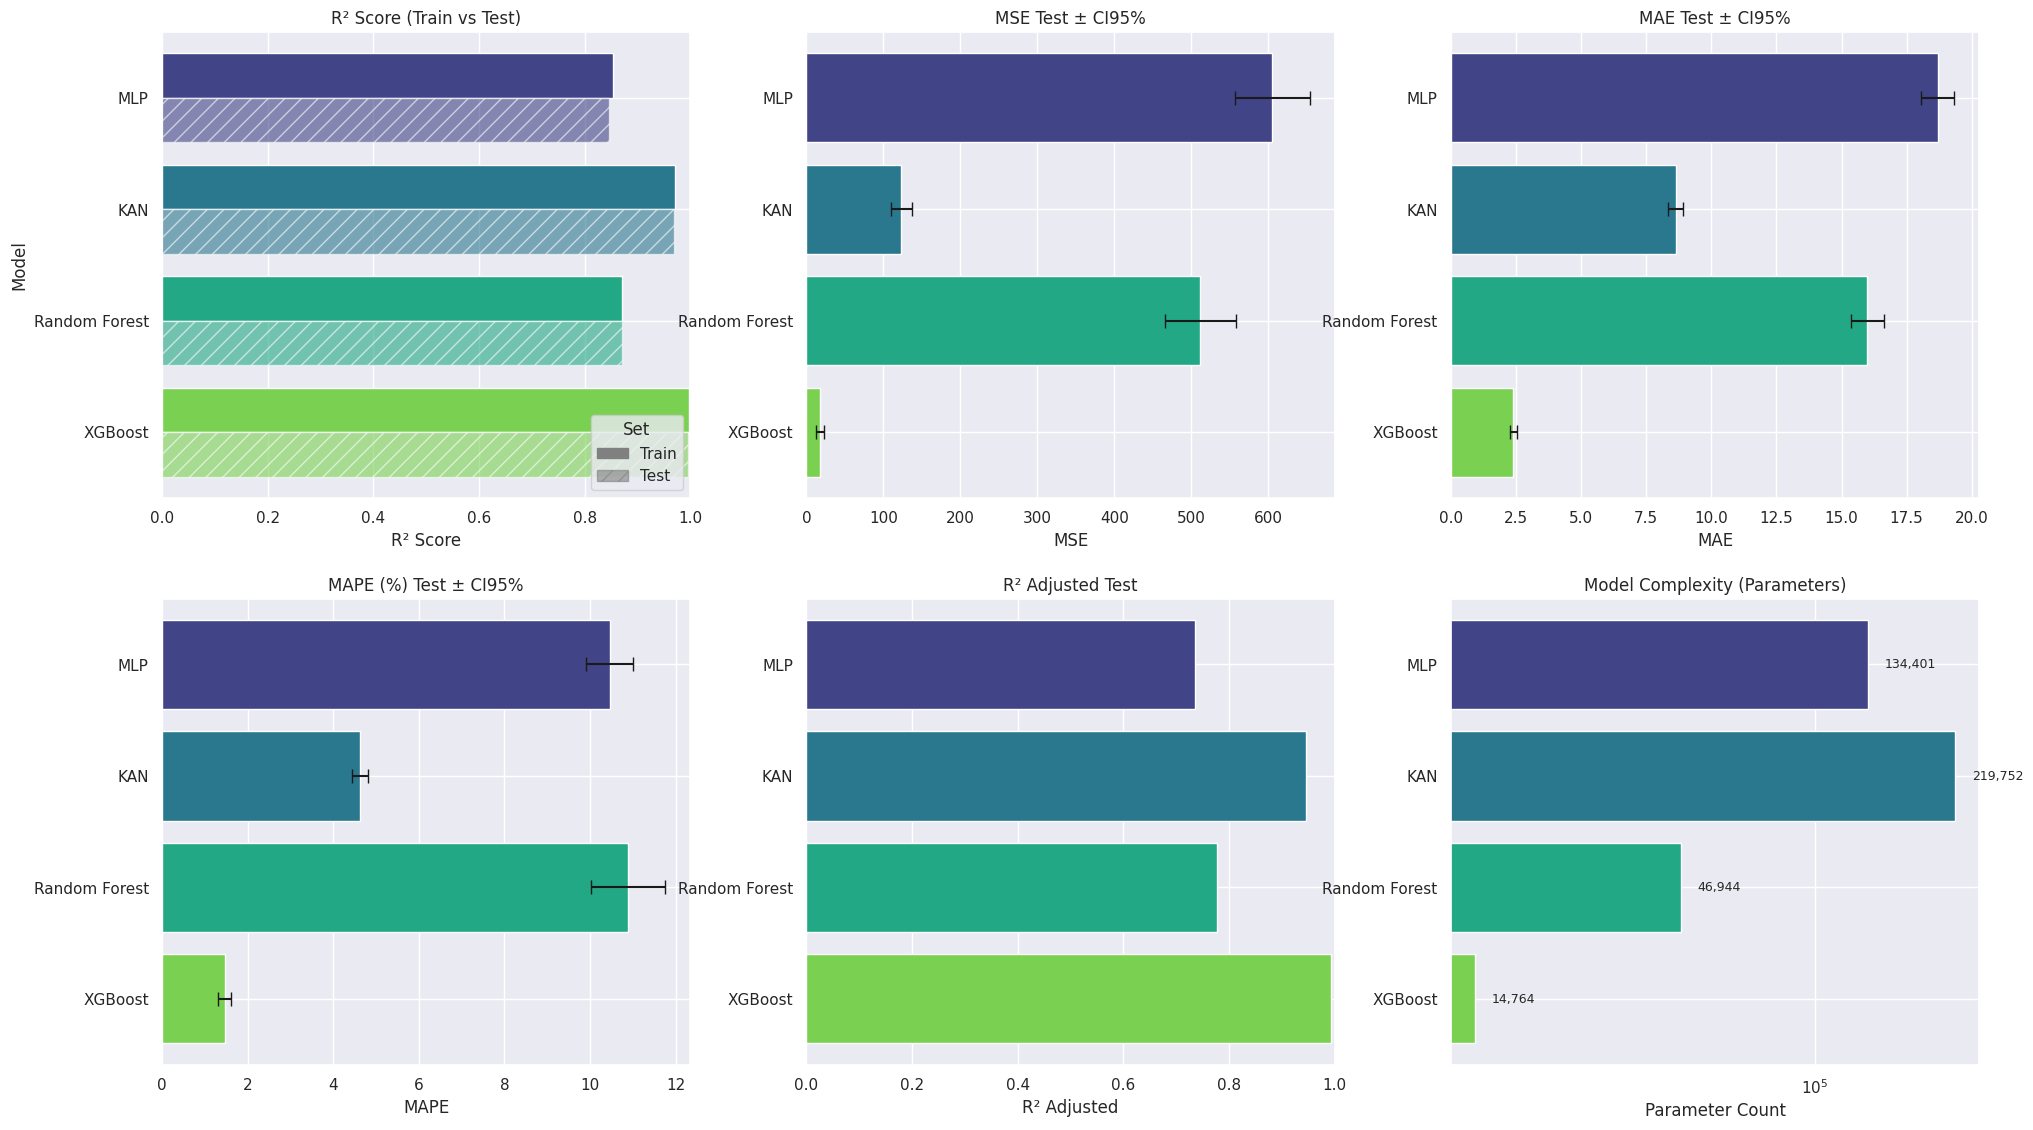
\includegraphics[width=1.0\textwidth]{img/comparison_car.png}
		\caption{Confronto visivo della complessitá e prestazioni dei modelli, utilizzando come metriche $R^2$, MSE, MAE, MAPE e $R^2$ aggiustato.}
		\label{fig:comparison_models}
	\end{figure}
	
	\begin{table}[H]
		\centering
		\small
		\label{tab:comparison_summary}
		\resizebox{\textwidth}{!}{
			\begin{tabular}{l
					c
					c
					c
					c
					c
					c
					c
					c}
				\toprule
				\textbf{Model} &
				\textbf{MSE Train (CI95\%)} &
				\textbf{MSE Test (CI95\%)} &
				\textbf{\(R^2\) Train} &
				\textbf{\(R^2\) Test} &
				\textbf{\(R^2\) Adj. Test} &
				\textbf{MAE Test} &
				\textbf{MAPE Test (CI95\%)} &
				\textbf{Max Error Test} \\
				\midrule
				MLP &
				589.72 (568.69 -- 610.76) &
				605.28 (556.94 -- 653.62) &
				0.8541 &
				0.8467 &
				0.8451 &
				18.69 &
				10.46 (9.91 -- 11.01) &
				136.45 \\
				KAN &
				119.10 (112.34 -- 125.86) &
				123.33 (110.11 -- 136.54) &
				0.9705 &
				0.9688 &
				0.9687 &
				8.63 &
				4.63 (4.45 -- 4.81) &
				108.35 \\
				RF &
				529.81 (510.10 -- 549.51) &
				511.72 (465.44 -- 558.00) &
				0.8717 &
				0.8704 &
				0.8654 &
				15.98 &
				10.89 (10.02 -- 11.76) &
				134.95 \\
				XGBoost &
				12.42 (11.22 -- 13.63) &
				17.52 (12.56 -- 22.48) &
				0.9970 &
				0.9956 &
				0.9968 &
				2.39 &
				1.46 (1.31 -- 1.62) &
				70.21 \\
				\bottomrule
			\end{tabular}
		}
		\caption{Tabella riassuntiva delle prestazioni (MSE con CI95\%, R$^2$, MAE, MAPE con CI95\%), Max Error e complessit\`a.}
	\end{table}
	
	\subsection{Risultati sperimentali}
	
	L’analisi dei risultati ha messo in evidenza differenze significative tra le reti neurali e i modelli ensemble, sia in termini di accuratezza sia di complessità computazionale. \\
	Per quanto riguarda le reti neurali, la \textbf{MLP} ha ottenuto un $R^2$ in test pari a $0.8467$ e un $R^2$ aggiustato di $0.8451$, con un errore quadratico medio (MSE) di circa $605$ e un errore assoluto medio (MAE) pari a $18.9$. Il valore di MAPE si attesta attorno al $10.5\%$, mentre il massimo errore assoluto in test ha raggiunto circa $136.5$. Queste prestazioni sono accettabili ma non particolarmente competitive, soprattutto considerando il numero relativamente elevato di parametri del modello (circa $134$k), che lo rende più pesante da addestrare e meno efficiente rispetto ad altre soluzioni. La \textbf{KAN} ha invece fornito risultati decisamente migliori, raggiungendo un $R^2$ test pari a $0.9688$ e un $R^2$ aggiustato di $0.9687$, con un MSE di $123$ e un MAE di $9.0$. Anche il MAPE, pari a circa $4.6\%$, conferma l’elevata accuratezza, mentre il massimo errore assoluto in test è stato di circa $108.3$. Questo incremento di precisione è stato ottenuto al costo di una complessità ancora maggiore, pari a circa $220$k parametri. Nel complesso, le reti neurali hanno mostrato un buon compromesso tra capacità di generalizzazione e accuratezza, ma con differenze marcate: l’MLP è risultato il meno competitivo, mentre KAN ha dimostrato una notevole capacità di modellare il problema, pur a fronte di un costo parametrico elevato. \\
	I modelli ensemble hanno mostrato un comportamento altrettanto interessante. La \textbf{Random Forest} ha raggiunto un $R^2$ test pari a $0.8704$ e un $R^2$ aggiustato di $0.8654$, con MSE di $511$ e MAE di $15.9$. Il MAPE ha raggiunto un valore medio del $10.9\%$, mentre il massimo errore assoluto è stato di circa $134.9$. Le sue prestazioni sono state quindi superiori a quelle dell’MLP, ma comunque meno accurate di quelle della KAN e soprattutto di XGBoost. La complessità del modello, stimata in circa $47$k parametri, lo rende più leggero delle reti neurali, ma non sufficientemente performante da rappresentare la soluzione migliore. \textbf{XGBoost}, al contrario, si è distinto come il modello più efficace: il suo $R^2$ test ha raggiunto il valore di $0.9956$ con un $R^2$ aggiustato di $0.9968$, accompagnato da un MSE di appena $17.5$ e un MAE pari a $2.5$. Il MAPE medio in test si attesta intorno all’$1.5\%$, e il massimo errore assoluto è stato limitato a circa $70.2$, valori che lo rendono nettamente superiore agli altri modelli. Oltre all’elevata precisione, un ulteriore vantaggio di XGBoost è l’efficienza, poiché la sua complessità è di soli $15$k parametri, rendendolo non solo il più accurato ma anche il più scalabile e pratico da utilizzare. \\
	
	\subsection{Selezione del miglior modello}
	Per identificare il modello più adatto al problema di regressione delle emissioni di CO2, è stata adottata una procedura che combina prestazione e complessità. Inizialmente, sono state definite le metriche di interesse e la rispettiva direzione di ottimizzazione, come mostrato di seguito: \\
	
	\begin{verbatim}
		metrics = {
			'MSE_Test'           : 'min',
			'MAE_Test'           : 'min',
			'MAPE_Test'          : 'min',
			'R2_Test'            : 'max',
			'R2_Adjusted_Test'   : 'max'
		}
	\end{verbatim}
	
	Per ciascuna metrica è stato calcolato il rank dei modelli (con il rank 1 che indica il migliore), tenendo conto della direzione appropriata (ascendente o discendente). Successivamente, è stato calcolato un \texttt{performance\_score} come media dei rank delle metriche di prestazione e un \texttt{Complexity\_rank} basato sul numero di parametri o nodi, dove il rank 1 corrisponde al modello meno complesso. \\
	Infine, sono stati combinati i punteggi di performance e complessità in base a diverse strategie di ponderazione. Sono stati usati l'Equal Weight (1:1), che somma direttamente il \texttt{performance\_score} e il \texttt{Complexity\_rank}, e le varianti con peso maggiore sulla complessità, ovvero il Complexity Weighted (1:2) e l'Extreme Complexity (1:3). È stato inoltre applicato un Pareto Approach (40:60), che combina i punteggi normalizzati con una ponderazione di 0.4 per la performance e 0.6 per la complessità. Per ogni metodo di aggregazione, il modello con il punteggio minimo è stato selezionato come il migliore. \\
	I risultati hanno mostrato una chiara prevalenza del modello XGBoost su tutte le metriche ponderate. Nello specifico, XGBoost è risultato il modello vincente in Equal Weight (1:1), Complexity Weighted (1:2), Extreme Complexity (1:3) e Pareto Approach (40:60). \\
	Di seguito la tabella riassuntiva con i valori principali usati per il ranking (valori ricavati dall'analisi finale):
	
	\begin{table}[H]
		\centering
		\setlength{\tabcolsep}{2pt}
		\small
		\begin{tabular}{lcccccc}
			\toprule
			\textbf{Model} & \textbf{Param\_Count} & \textbf{Avg\_Perf} & \textbf{Compl\_Rank} & \textbf{Equal\_Rank} & \textbf{Ext\_Rank} & \textbf{Pareto\_Rank} \\
			\midrule
			MLP           & 134,401 & 3.83 & 3 & 4 & 3 & 4 \\
			KAN           & 219,752 & 2.00 & 4 & 3 & 4 & 3 \\
			XGB 		  & 14,764  & 1.00 & 1 & 1 & 1 & 1 \\
			RF 			  & 46,944  & 3.17 & 2 & 2 & 2 & 2 \\
			\bottomrule
		\end{tabular}
		\caption{Riepilogo ranking: conteggio parametri, performance media (rank-based) e ranks per metodo di aggregazione.}
	\end{table}
	
	\subsubsection{Conclusioni}
	L'analisi ha portato a individuare XGBoost come il più adatto al problema. Questo modello non solo ha ottenuto le migliori performance assolute su tutte le metriche di regressione, ma ha anche la complessità stimata più bassa, rendendolo la scelta ideale per un deployment operativo. La rete KAN ha raggiunto un buon compromesso in termini di performance, sebbene la sua complessità stimata sia risultata elevata in rapporto al beneficio predittivo assoluto. L'MLP, pur avendo il maggior numero di parametri di XGBoost, ha conseguito performance inferiori rispetto ad esso in termini di MSE e MAE. Il Random Forest ha fornito risultati stabili e prestazioni intermedie, ma non è riuscito a superare XGBoost nel compromesso tra performance e complessità. \\
	La classifica dei tre migliori modelli, secondo il criterio \emph{complexity-weighted} (dal migliore al peggiore), è la seguente:
	\begin{enumerate}
		\item XGBoost (Parametri: 14,764 | MSE Test: 17.52)
		\item Random Forest (Parametri: 46,944 | MSE Test: 511.72)
		\item MLP (Parametri: 134,401 | MSE Test: 605.28)
	\end{enumerate}
	
	\section{Studio di ablazione}
	
	\subsection{Ablation study: L1 pruning su MLP e KAN}
	L'obiettivo è misurare il compromesso tra compressione del modello (numero di parametri attivi / rapporto di compressione) ed il mantenimento delle prestazioni (MSE, MAE, \(R^2\), MAPE).
	
	\subsubsection{Metodologia}
	La tecnica di pruning impiegata è il L1 post-training pruning, applicato ai pesi lineari della MLP ed ai coefficienti spline della KAN. Sono stati testati diversi pruning ratios, specificamente l'insieme ${0.0,0.1,0.2,0.3,0.4,0.5,0.6,0.7,0.8,0.9,0.95}$. Ciascuna versione del modello potata è stata valutata sia sul test set che sul train set utilizzando le metriche MSE, MAE, MAPE, $R^2$ e max error. Per ogni configurazione, sono stati calcolati il numero totale di parametri, il numero di parametri attivi post-pruning ed il rapporto di compressione. Per interpretare i risultati, sono state definite alcune definizioni operative. La baseline è il modello non potato (pruning ratio $= 0.0$). Il punto di degrado significativo è il primo pruning ratio che comporta una perdita relativa in $R^2$ superiore al 5\% rispetto alla baseline. Il best trade-off è il punto di massima compressione che causa una perdita relativa in $R^2$ inferiore o uguale al 2\%.
	
	\subsubsection{Figura riassuntiva}
	\begin{figure}[H]
		\centering
		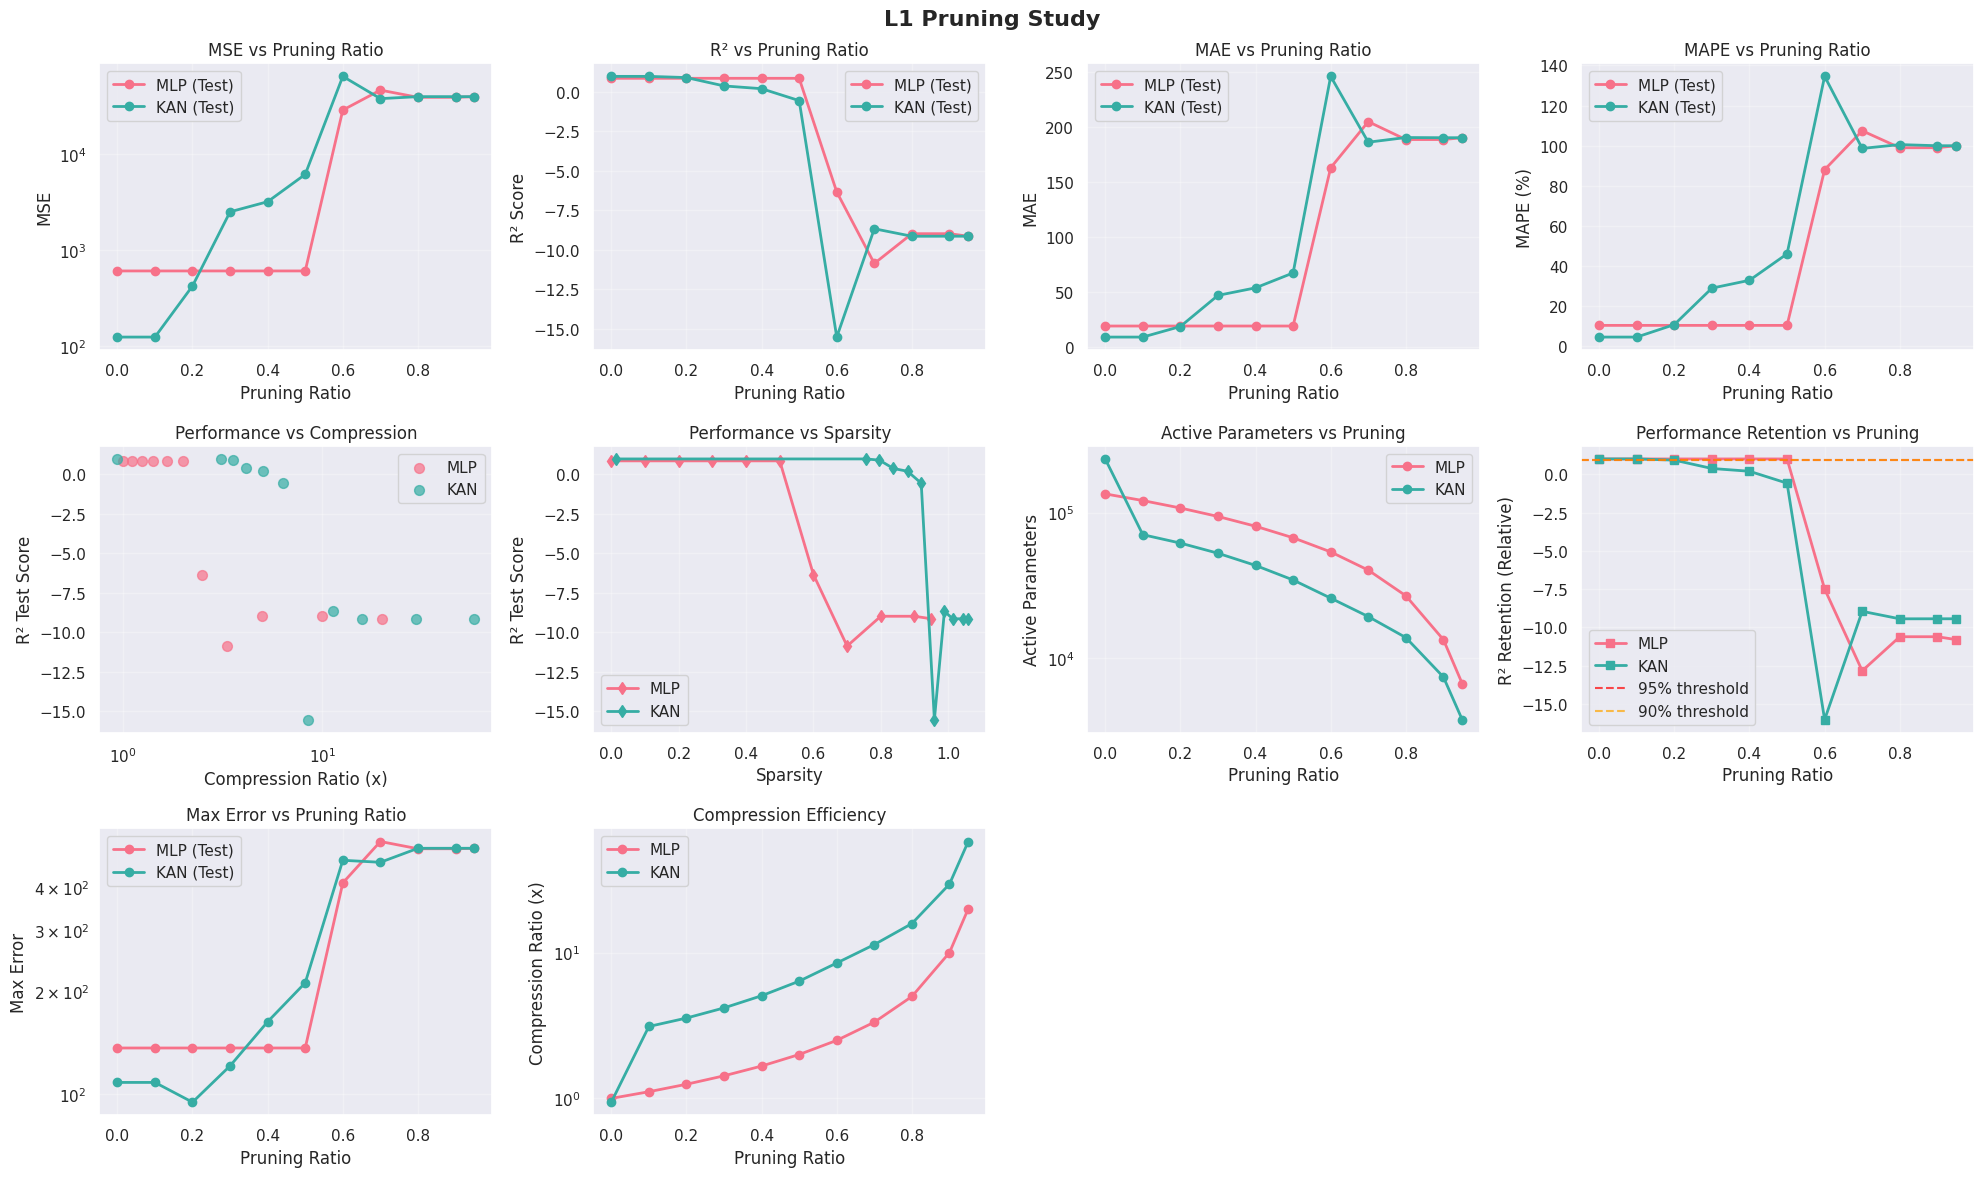
\includegraphics[width=1.0\textwidth]{img/abl_kanvsmlp_car.png}
		\caption{Risultati dello studio L1 pruning per MLP e KAN, utilizzando metriche principali e indicatori di compressione (MSE, \(R^2\), MAE, MAPE, max error, sparsitá, parametri attivi, performance retention).}
	\end{figure}
	
	\subsubsection{Risultati}
	\begin{table}[H]
		\centering
		\setlength{\tabcolsep}{4pt}
		\begin{tabular}{lcccc}
			\toprule
			\textbf{Model} & \textbf{Total params} & \textbf{Baseline $R^2$} & \textbf{Best trade-off} & \textbf{Sign. degr.} \\
			\midrule
			MLP & 134\,401  & 0.8467 & 50\% pruning (compression $\approx 2.0\times$) & 60\% pruning \\
			KAN & 219\,752  & 0.9688 & 10\% pruning (compression $\approx 3.1\times$) & 20\% pruning \\
			\bottomrule
		\end{tabular}
		\caption{Riepilogo dei punti di trade-off e dei punti di degrado osservati nello studio L1 pruning.}
	\end{table}
	
	La MLP ha una baseline \(R^2=0.8467\). Fino a un pruning del 50\%, non si osserva una perdita significativa in \(R^2\), rappresentando il miglior trade-off con una compressione di circa $2.0\times$. Il modello inizia a mostrare un degrado significativo intorno al 60\% di pruning, dove MSE e MAE aumentano drasticamente e l'\(R^2\) diventa negativo per pruning più aggressivi. La compressione massima sperimentata è di circa $20\times$ (pruning del 95\%), ma a questo livello la performance è inutilizzabile. \\
	La KAN, con una baseline \(R^2=0.9688\), ha mostrato il suo miglior trade-off empirico con un pruning del 10\% con una compressione di circa $3.1\times$, mantenendo la performance praticamente invariata. Il degrado significativo compare già a circa il 20\% di pruning, oltre il quale MSE e MAE aumentano rapidamente. La massima compressione sperimentata è di circa $57.8\times$ (pruning del 95\%), ma con una perdita di performance molto elevata. \\
	
	\subsection{Ablation study: ensemble pruning su Random Forest e XGBoost}
	Lo scopo è valutare il compromesso tra riduzione del modello (numero di alberi / rounds) e mantenimento delle prestazioni (qui riportate con metriche di regressione — MSE, \(R^2\), MAE.
	
	\subsubsection{Metodologia}
	La metodologia di pruning varia per i due modelli. Per il Random Forest, è stato utilizzato un Rank-Based Pruning: gli alberi sono stati ordinati per importanza e quelli meno rilevanti sono stati rimossi fino a raggiungere il \texttt{pruning\_ratio} desiderato. Per XGBoost, si è optato per un Cumulative Pruning, mantenendo solo le prime iterazioni di boosting fino al numero corrispondente a \((1 - \texttt{pruning\_ratio})\) della lunghezza originale, troncando di fatto la sequenza di boosting. Anche in questo caso, i pruning ratios testati sono stati ${0.0,0.1,0.2,0.3,0.4,0.5,0.6,0.7,0.8,0.9,0.95}$. Per ogni versione potata, sono stati calcolati il numero totale e residuo di alberi, il rapporto di compressione e le metriche di performance su train e test set. Le definizioni operative di baseline, punto di degrado significativo ($R^2 >5\%$) e best trade-off ($R^2 \le 2\%$) sono rimaste le medesime.
	
	\subsubsection{Figura riassuntiva}
	\begin{figure}[H]
		\centering
		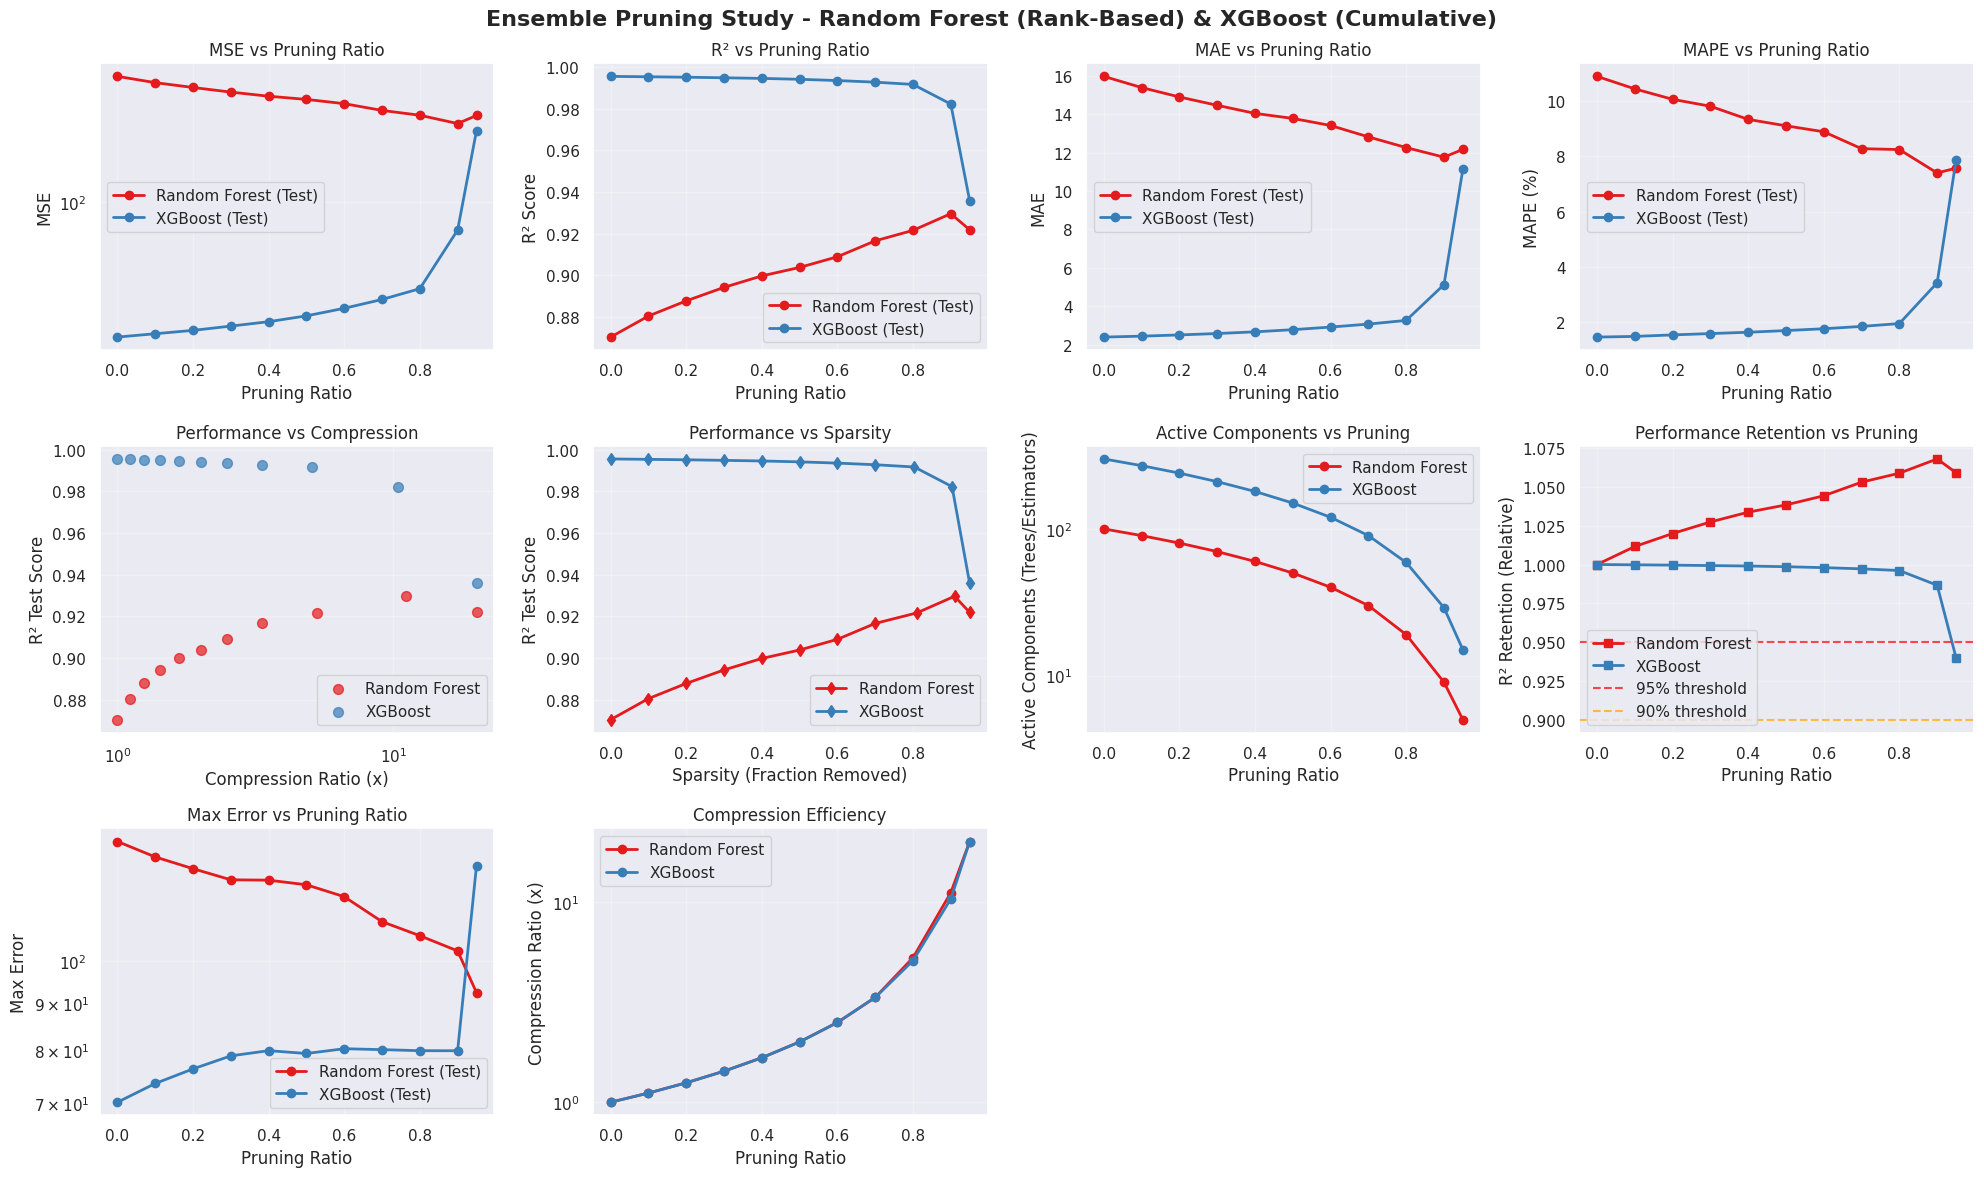
\includegraphics[width=\textwidth]{img/abl_xgbvsrf_car.png}
		\caption{Risultati dello studio di pruning per Random Forest (rank-based) e XGBoost (cumulative), utilizzando metriche principali e indicatori di compressione (MSE, \(R^2\), MAE, MAPE, max error, sparsitá, parametri attivi, performance retention).}
	\end{figure}
	
	\subsubsection{Risultati}
	\begin{table}[H]
		\centering
		\setlength{\tabcolsep}{4pt}
		\begin{tabular}{lcccc}
			\toprule
			\textbf{Model} & \textbf{Total components} & \textbf{Baseline (\(R^2\))} & \textbf{Best trade-off} & \textbf{Sign. degr.} \\
			\midrule
			RF        & 100 trees & 0.8704 & 95\% (compression 20.0×) & no degr. rilevata \\
			XGB       & 300 trees & 0.9956 & 90\% (compression 10.3x) & 95\% pruning \\
			\bottomrule
		\end{tabular}
		\caption{Riepilogo sintetico dei punti di trade-off osservati per i due ensemble.}
	\end{table}
	
	XGBoost ha dimostrato di essere molto robusto anche con pruning aggressivi, mantenendo una perdita trascurabile in \(R^2\) fino ad una riduzione del 70-80\% degli estimators. Il miglior trade-off empirico si è verificato al 90\% di pruning, mantenendo 29 alberi su 300, con una compressione di circa $10.3\times$ ed una perdita relativa di \(R^2\) di appena l'1.3\%. Oltre questa soglia, le performance calano rapidamente. \\
	Nel caso del Random Forest, il pruning rank-based ha mostrato una tendenza a mantenere o addirittura a migliorare leggermente la generalizzazione, riducendo l'overfitting. L'esperimento ha rivelato che il modello rimane stabile anche con pruning aggressivi: mantenendo solo 5 alberi su 100 (95\% di pruning, compressione $20\times$), l'\(R^2\) sul test set non peggiora e, in alcuni casi, migliora rispetto alla baseline.
	
	\subsection{Ablation study — Confronto complessivo (Neural Networks vs Ensemble)}
	Per il confronto, sono stati considerati pruning ratios tipici: 30\%, 50\%, 70\%, 90\%.  
	
	\subsubsection{Metriche e output considerati}
	Per ogni modello sono state raccolte le seguenti misure:
	\begin{itemize}
		\item \textbf{\(R^2\)} (test);
		\item \textbf{MSE} (test);
		\item \textbf{MAE} (test);
		\item \textbf{MAPE} (test);
		\item \textbf{Compression ratio}: rapporto tra dimensione modello baseline e modello pruned;
		\item statistiche di performance retention (\(R^2\) pruned / baseline).
	\end{itemize}
	
	\subsubsection{Figure riassuntive}
	\begin{figure}[H]
		\centering
		\begin{minipage}{0.49\textwidth}
			\centering
			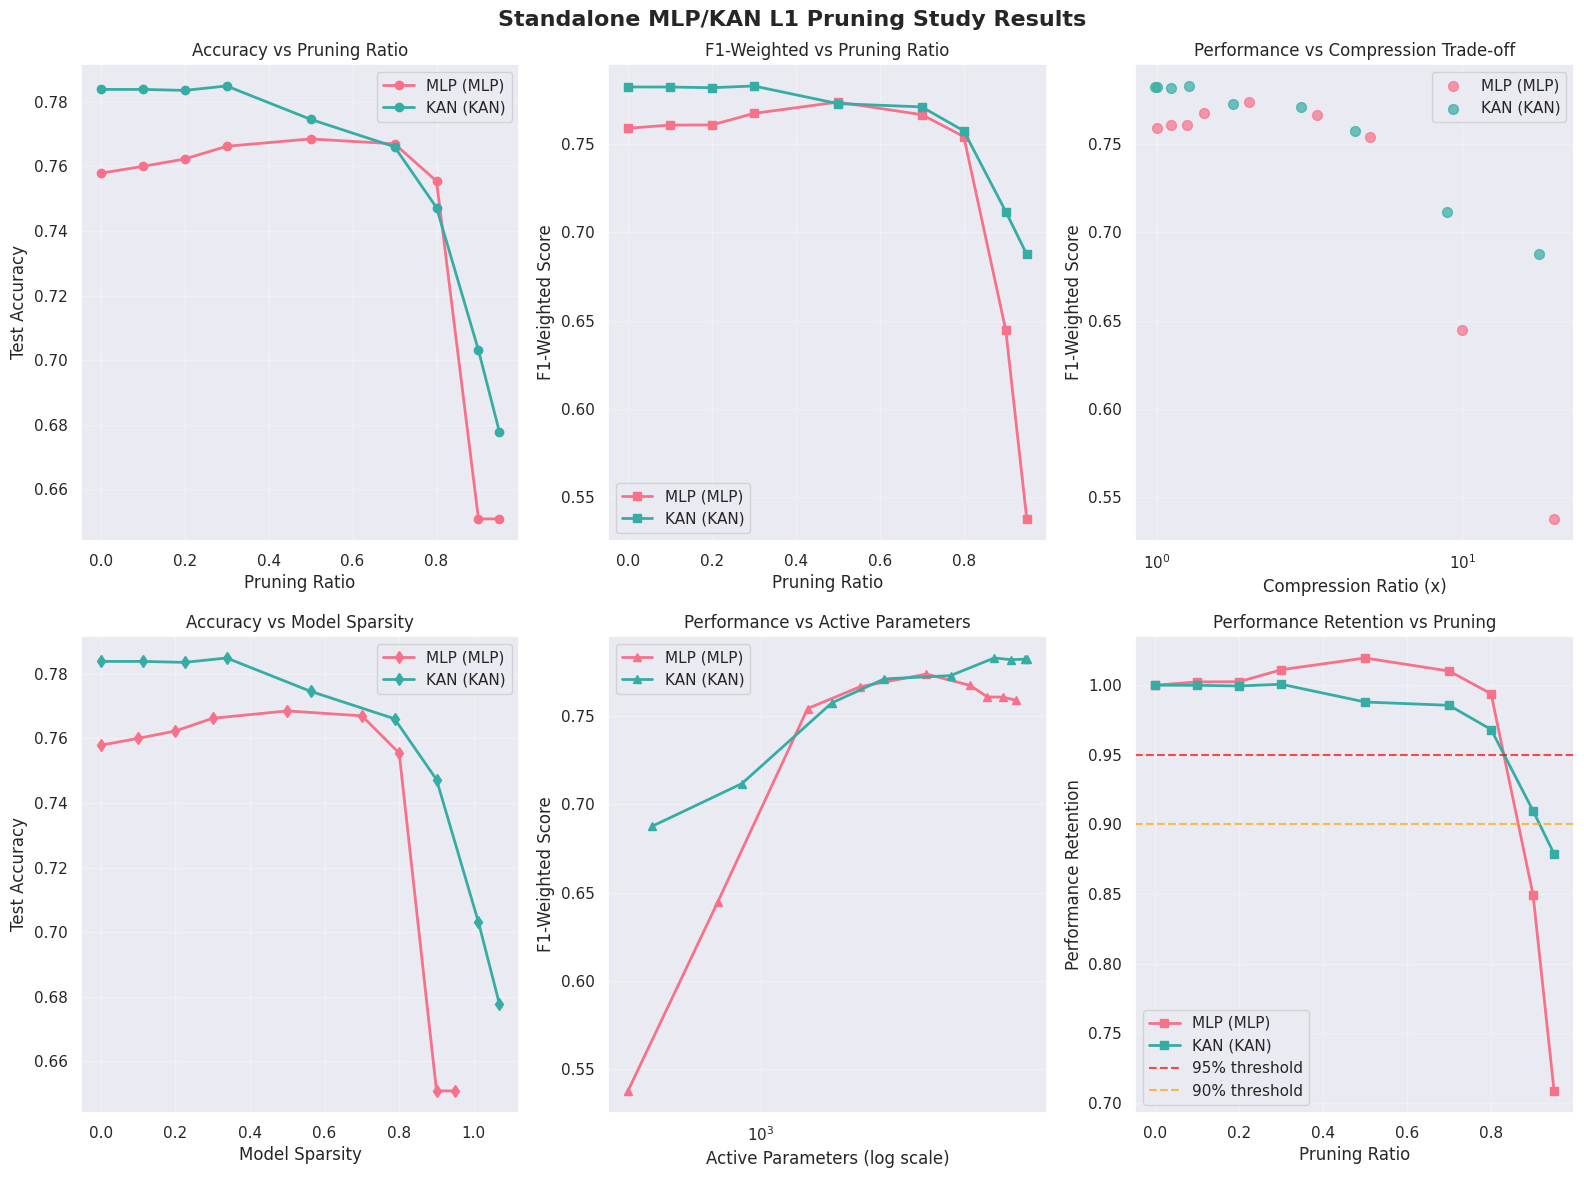
\includegraphics[width=\linewidth]{img/abl_kanvsmlp_pm.png}
			\caption*{A: Studio di Ablazione MLP e KAN (L1 pruning).}
		\end{minipage}\hfill
		\begin{minipage}{0.49\textwidth}
			\centering
			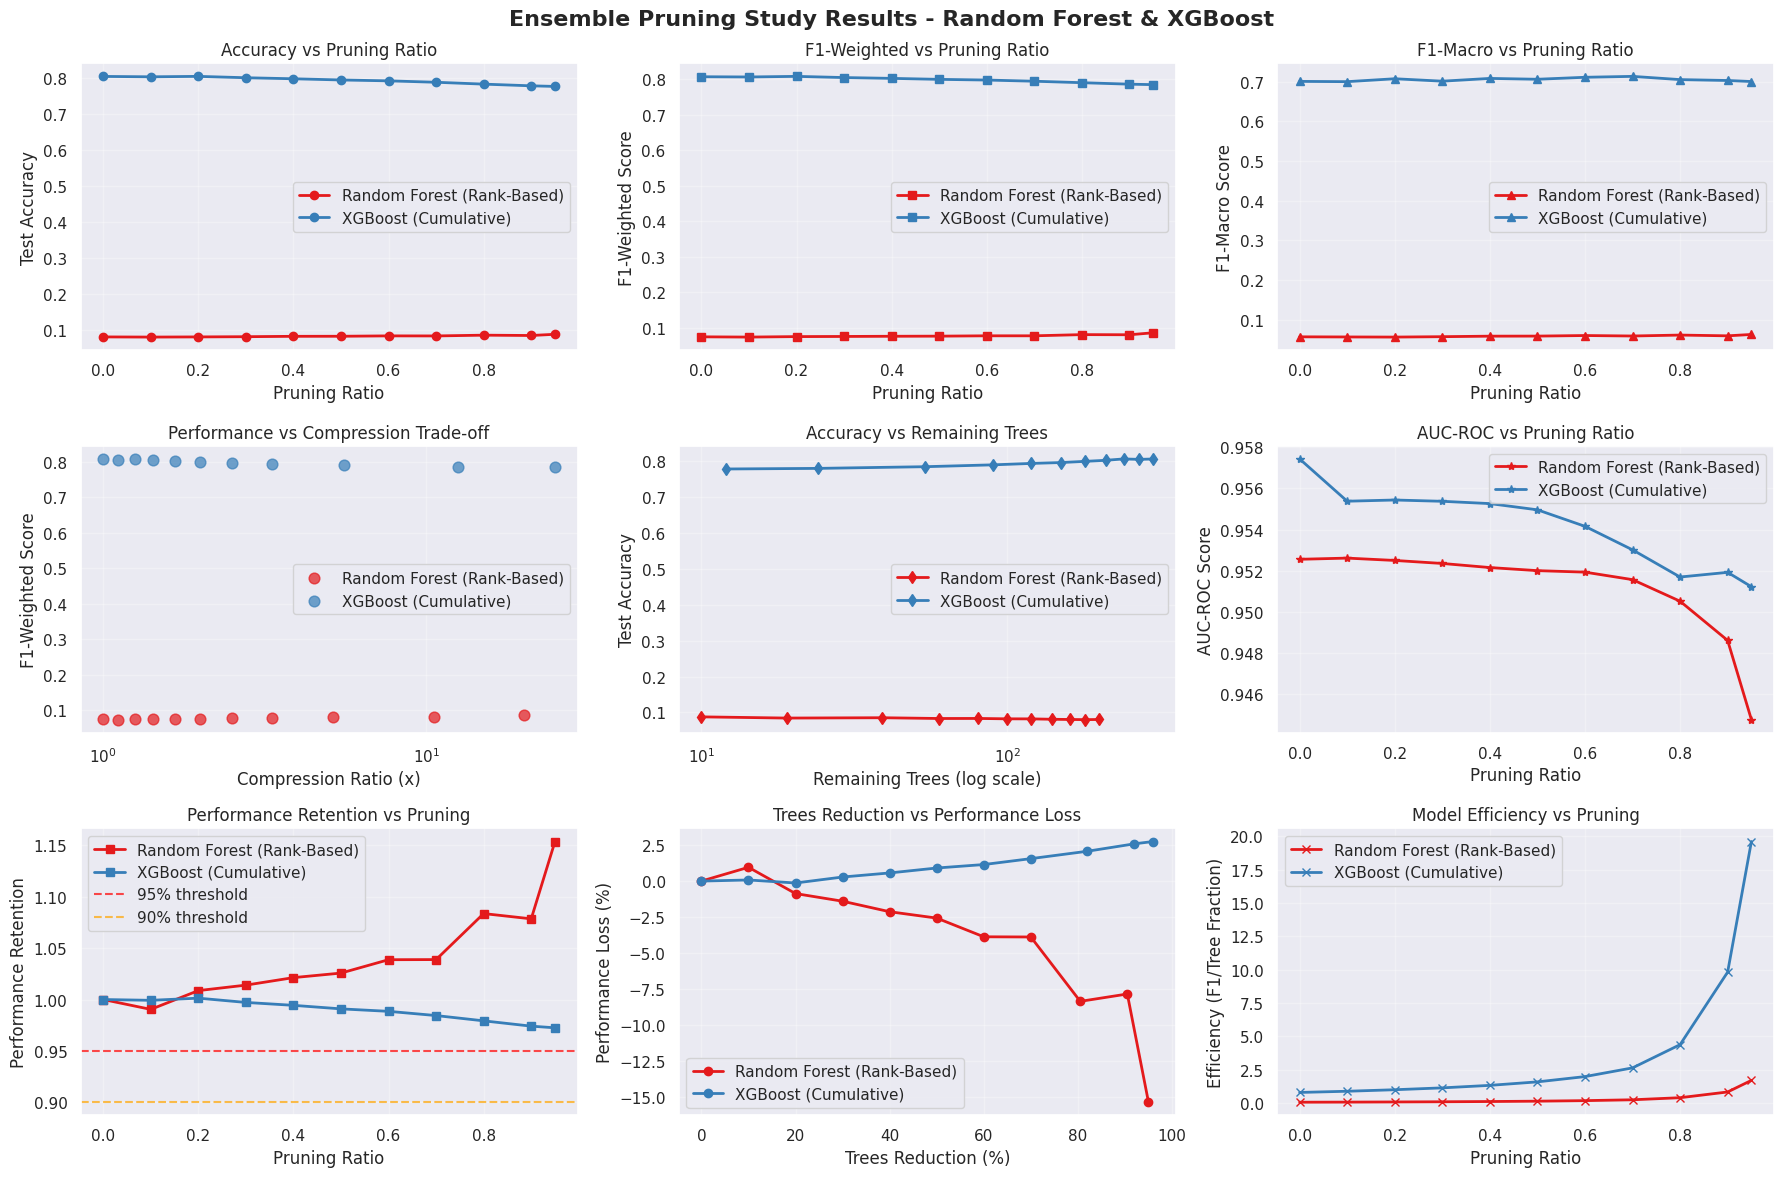
\includegraphics[width=\linewidth]{img/abl_xgbvsrf_pm.png}
			\caption*{B: Studio di Ablazione Random Forest (Rank-based) e XGBoost (cumulative).}
		\end{minipage}
		\caption{Risultati sintetici degli studi di ablazione.}
	\end{figure}
	
	\subsubsection{Riepilogo}
	\begin{table}[H]
		\centering
		\begin{tabular}{lccc}
			\toprule
			\textbf{Model} & \textbf{Baseline \(R^2\)} & \textbf{Best trade-off} & \textbf{Compression} \\
			\midrule
			XGB           & 0.9956 & 0.9823 @ 90\% pr & \(\approx 10.3\times\) \\
			RF            & 0.8704 & 0.9219 @ 95\% pr & \(\approx 20.0\times\) \\
			MLP           & 0.8467 & 0.8467 @ 50\% pr & \(\approx 2.0\times\) \\
			KAN           & 0.9688 & 0.9688 @ 10\% pr & \(\approx 3.1\times\) \\
			\bottomrule
		\end{tabular}
		\caption{Riepilogo sintetico dei principali punti di trade-off e compressione.}
	\end{table}
	
	\subsubsection{Confronto su soglie tipiche (30\%, 50\%, 70\%, 90\%)}
	Ad un pruning del 30\%, Random Forest e XGBoost mantengono le prestazioni quasi invariate (\(R^2 \approx 0.894\) e 0.995 rispettivamente), mentre la MLP rimane stabile (\(R^2 = 0.8467\)). La KAN, al contrario, degrada molto rapidamente (\(R^2 \approx 0.364\)). \\
	Con un pruning del 50\%, XGBoost conserva un \(R^2 \approx 0.994\), e Random Forest migliora ulteriormente la generalizzazione (\(R^2 \approx 0.904\)). La MLP resta stabile, mentre la KAN crolla sotto lo 0. \\
	Al 70\% di pruning, XGBoost si dimostra ancora robusto (\(R^2 \approx 0.993\), con una compressione di $3.3\times$. Il Random Forest continua a migliorare (\(R^2 \approx 0.917\)), mentre la MLP e la KAN subiscono un forte degrado, con un $R^2$ negativo. \\
	A un pruning del 90\%, Random Forest mostra la migliore performance in termini di retention (\(R^2 \approx 0.9296\)) con una compressione di $11\times$. Anche XGBoost mantiene buone prestazioni (\(R^2 \approx 0.9823\), compressione $10.3\times$), mentre MLP e KAN risultano completamente compromessi.
	
	\subsubsection{Conclusioni}
	\begin{enumerate}
		\item XGBoost si conferma il modello più stabile sotto pruning aggressivo, mantenendo un \(R^2 > 0.98\) ed una compressione di circa $10.3\times$ fino ad un pruning del 90\%.
		\item Per il Random Forest, il pruning rank-based porta ad un notevole miglioramento della generalizzazione, con un \(R^2\) che sale a $0.9296$ con un pruning del 90\% ed una compressione di circa $11.1\times$.
		\item La MLP tollera il pruning fino al 50\% (compressione $2\times$) senza perdita di $R^2$, ma degrada rapidamente oltre questa soglia.
		\item La KAN è estremamente sensibile al pruning: già al 20\% l'$R^2$ scende a circa $0.893$, e crolla sotto lo 0 oltre il 40-50\%.
	\end{enumerate}
	
	\chapter{Secondo Caso Studio: Classificazione di PM2.5}
	
	\section{Introduzione}
	Il presente caso studio si occupa della classificazione dei livelli di PM2.5, utilizzando un dataset nazionale di misurazioni orarie provenienti da 453 città indiane nel periodo 2010-2023, arricchito con variabili meteorologiche. I dati utilizzati sono stati forniti dal \textit{Central Pollution Control Board} (CPCB), portale ufficiale del Governo indiano per il monitoraggio e il controllo dell’inquinamento, resi pubblicamente disponibili sul sito istituzionale \url{https://cpcb.nic.in}. A differenza di altri capitoli, qui le operazioni di caricamento, pulizia, gestione dei missing, individuazione degli outlier, ricampionamento ed aggregazione costituiscono parte integrante del workflow sperimentale e sono descritte nelle sezioni successive. \\
	Gli obiettivi del caso studio sono: (i) trasformare la previsione delle concentrazioni di PM2.5 in un problema di classificazione ordinata secondo le classi AQI (GOOD $\rightarrow$ HAZARDOUS) per garantire interpretabilità applicativa; (ii) confrontare i quattro modelli precedentemente definiti e valutare l’effetto delle scelte di preprocessing, del feature engineering temporale (lag, componenti cicliche), delle tecniche di bilanciamento e delle procedure di ottimizzazione sugli indicatori di performance. Per una stima robusta della generalizzazione si utilizza una validazione con criterio temporale e si forniscono intervalli di confidenza per le principali metriche. \\
	Nel capitolo vengono presentati, in sequenza: una nota sulle sorgenti e la composizione del dataset; la pipeline di preprocessing e le scelte di indicizzazione/aggregazione; le tecniche di feature engineering e la discretizzazione in classi AQI; la strategia di training e ottimizzazione; i risultati quantitativi (metriche aggregate con CI95\% e confusion matrix); infine gli studi di ablazione e le considerazioni finali sul compromesso tra performance e complessità per scenari di deployment.
	
	\section{Data preparation}
	
	Questa sezione descrive in dettaglio le operazioni svolte per il caricamento, la normalizzazione, la pulizia e l'arricchimento del dataset utilizzato nel caso studio. Lo scopo principale della fase di Data preparation è trasformare i dati grezzi in una rappresentazione coerente, completa e utilizzabile per la successiva fase di allenamento.
	
	\subsection{Fonti e descrizione generale del dataset}
	Il dataset principale utilizzato nello studio raccoglie misurazioni relative alla qualità dell'aria in numerose stazioni di monitoraggio presenti in 453 città indiane per il periodo temporale 2010-2023. Le osservazioni includono sia concentrazioni di inquinanti sia variabili meteorologiche ed ambientali.\\
	Un file ausiliario, denominato stations\_info.csv, contiene la mappatura tra i file contenenti le misure e informazioni di contesto (stato, città, agenzia responsabile, data di inizio rilevamento), permettendo in tal modo una gestione centralizzata dei metadati associati alle stazioni di monitoraggio.
	
	\subsection{Caricamento dati e organizzazione iniziale}
	Il caricamento del dataset è stato effettuato tramite la lettura dei file compressi estratti in una directory locale o su Google Colab. Per ogni file contenente le misure di una singola stazione, sono state eseguite diverse operazioni. Innanzitutto, il contenuto di ciascun archivio ZIP è stato estratto in una directory strutturata per stato. In seguito, sono stati letti i metadati dal file \texttt{stations\_info.csv} e sono state rimosse le colonne non necessarie per l'analisi, al fine di semplificare la tabella. Infine, è stato costruito un insieme aggregato: per ogni stato, sono stati individuati automaticamente tutti i file CSV con il prefisso identificativo dello stato, ogni file è stato letto e arricchito con le colonne "city" e "state", e tutte le tabelle sono state concatenate in un unico DataFrame nazionale. \\
	Il risultato di questa fase è un DataFrame unico che contiene le misurazioni orarie con colonne per le concentrazioni degli inquinanti, le variabili meteorologiche e gli identificatori geografici.
	
	\subsection{Indicizzazione temporale}
	Nel dataset originale, le finestre temporali di misurazione sono definite dalle colonne "From Date" e "To Date". Per semplificare la gestione delle serie storiche, la colonna "From Date" è stata convertita in tipo datetime, quindi rinominata in "datetime" ed impostata come indice temporale del DataFrame. La colonna "To Date", ridondante per l'analisi, è stata rimossa. Questa trasformazione permette di sfruttare le funzionalità native di raggruppamento e ricampionamento temporale offerte dalle librerie per la manipolazione delle serie storiche.
	
	\subsection{Riduzione e unificazione di feature ridondanti}
	Durante l'esplorazione iniziale è emersa la presenza di colonne duplicate o varianti dello stesso nome, come "Ozone (ug/m3)" e "Ozone (ppb)". Per evitare rappresentazioni inconsistenti della stessa grandezza, sono state seguite alcune operazioni. In primo luogo, sono stati identificati i gruppi di colonne equivalenti tramite l'analisi grafica dei trend (andamento delle medie annue) ed il confronto delle statistiche di base. Successivamente, è stato definito un mapping di riduzione, ad esempio aggregando tutte le varianti di Xilene in una singola colonna comune. Infine, per ogni gruppo, i valori non nulli provenienti dalle colonne secondarie sono stati trasferiti nella colonna principale, e le colonne ridondanti sono state eliminate.
	
	\begin{figure}[H]
		\centering
		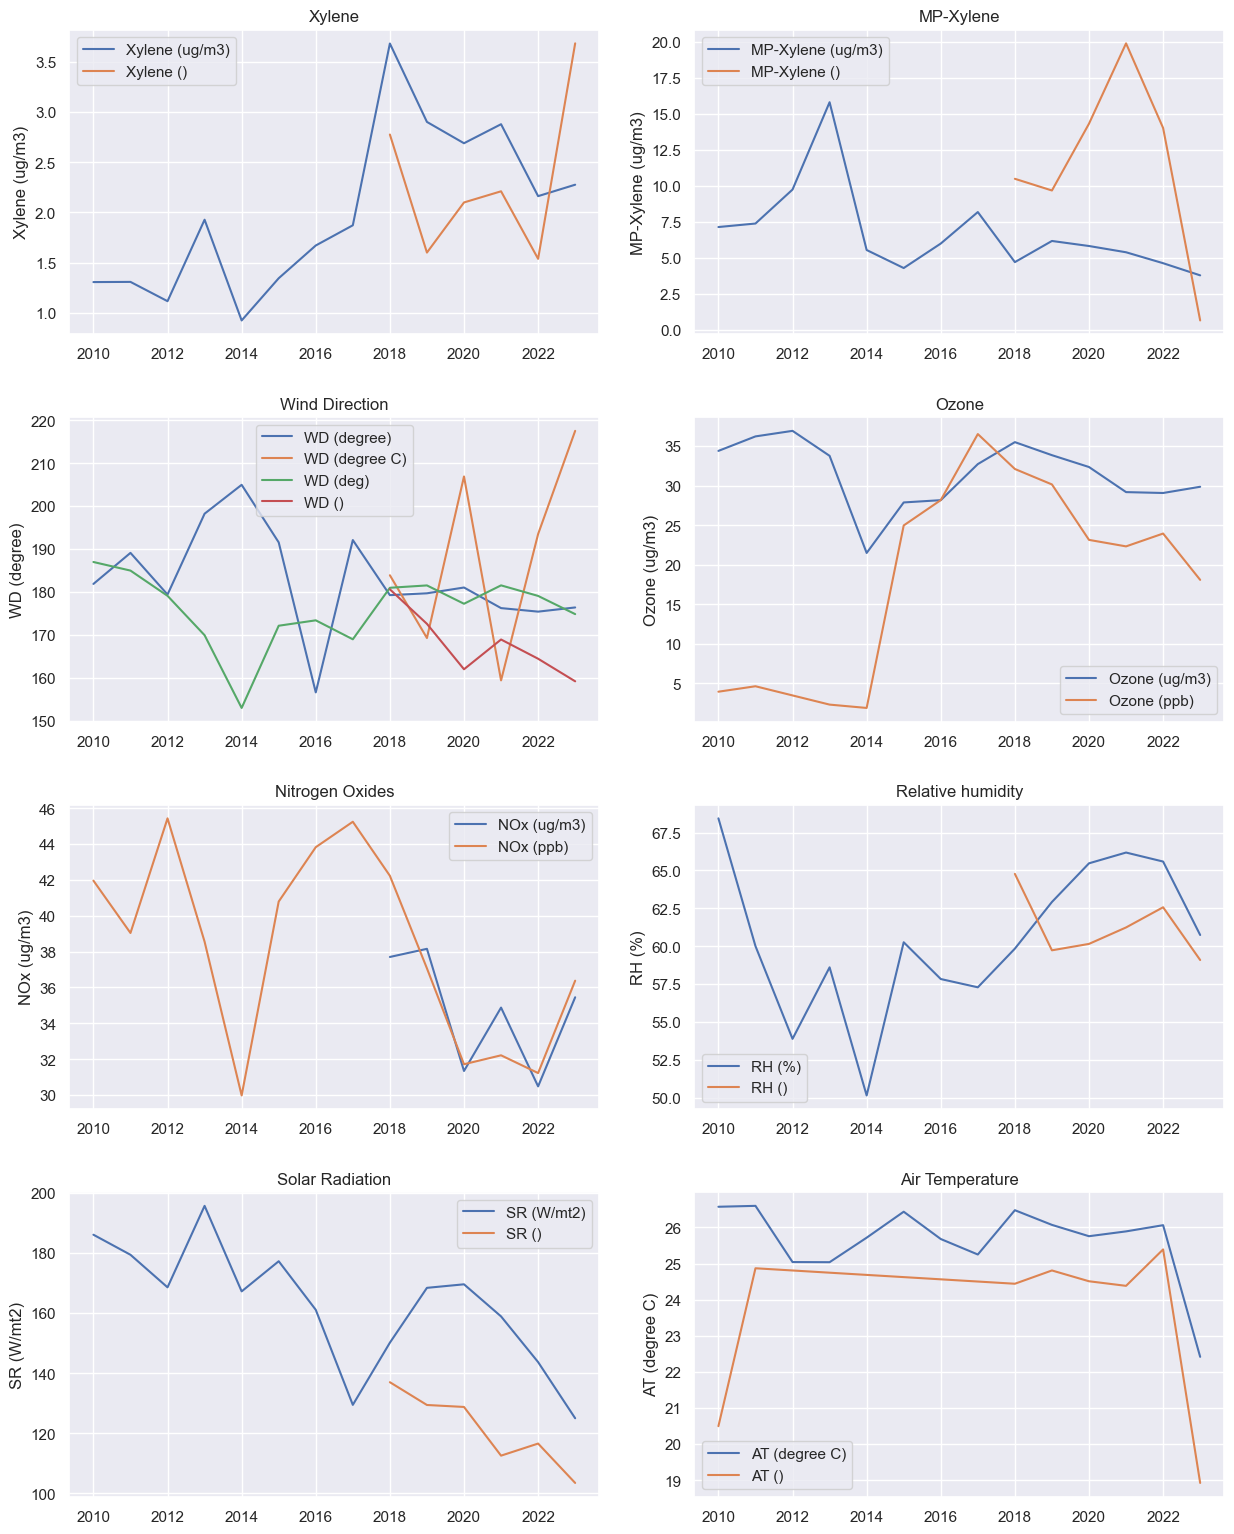
\includegraphics[width=1.0\textwidth]{img/feat_red_pm.png}
		\caption{Similaritá delle features - Analisi medie annue}
	\end{figure}
	
	\subsection{Verifica e gestione dei valori mancanti}
	La quantificazione dei valori mancanti è stata effettuata calcolando il numero assoluto e la percentuale di missing per ogni variabile.
	
	\begin{figure}[H]
		\centering
		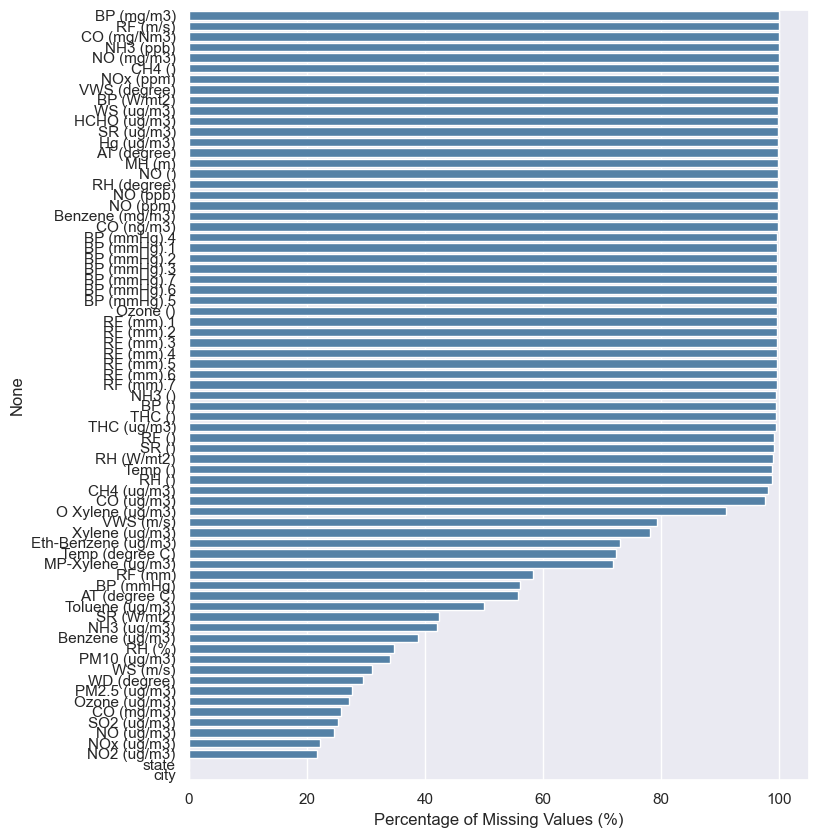
\includegraphics[width=1.0\textwidth]{img/miss_value_pm.png}
		\caption{Percentuali dei Valori Mancanti.}
	\end{figure}
	
	Sono stati applicati i seguenti criteri: la rimozione delle osservazioni completamente vuote e delle colonne completamente vuote; l'eliminazione delle colonne con una proporzione di valori mancanti superiore al 40\%, una soglia scelta per bilanciare la perdita informativa con la robustezza statistica; e, per le restanti colonne numeriche, la sostituzione dei valori NaN. Questa sostituzione è stata eseguita tramite il metodo di interpolazione \texttt{forward-fill} (propagazione dell'ultimo valore valido), seguita da una sostituzione tramite la media per eventuali valori mancanti residui. Questa strategia è comunemente adottata nelle serie temporali, poiché preserva la dinamica locale dei segnali ed evita l'introduzione di discontinuità.
	
	\subsection{Analisi esplorativa e selezione delle feature rilevanti}
	Per esplorare le relazioni e le correlazioni tra le variabili, sono state eseguite diverse analisi. Sono state calcolate le medie su diverse frequenze temporali (giorno, mese, anno) per visualizzare i trend con grafici a linee. È stato utilizzato il pairplot per ispezionare le relazioni bivariate e le distribuzioni univariate. Inoltre, è stata costruita la matrice di correlazione e visualizzata tramite una heatmap per quantificare le correlazioni lineari, identificando come potenziali feature rilevanti quelle con una correlazione assoluta superiore a 0.4 con "PM2.5".
	
	\begin{figure}[H]
		\centering
		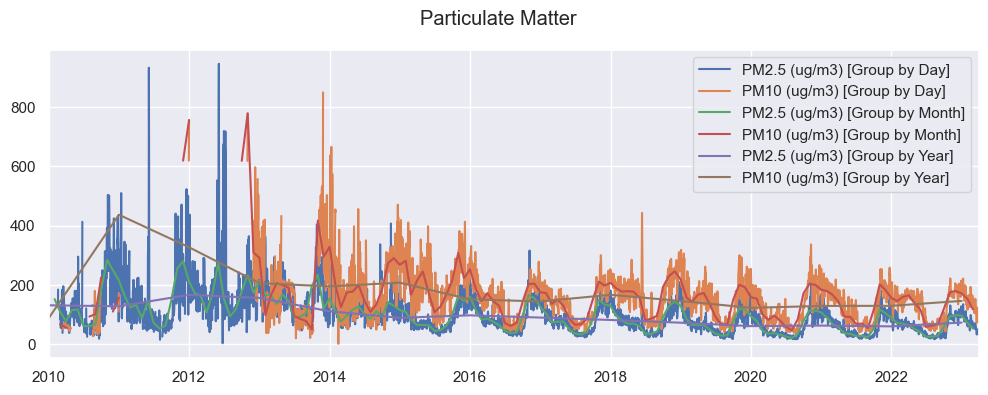
\includegraphics[width=1.0\textwidth]{img/pm_trend_pm.png}
		\caption{Analisi dei trend giornalieri, mensili e annuali per il Particolato.}
	\end{figure}
	\begin{figure}[H]
		\centering
		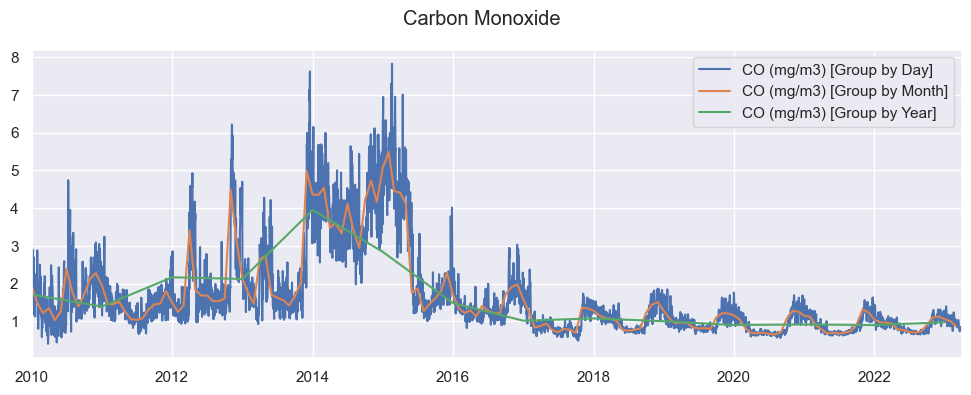
\includegraphics[width=1.0\textwidth]{img/carbon_trend_pm.png}
		\caption{Analisi dei trend giornalieri, mensili e annuali per il Monossido di carbonio.}
	\end{figure}
	\begin{figure}[H]
		\centering
		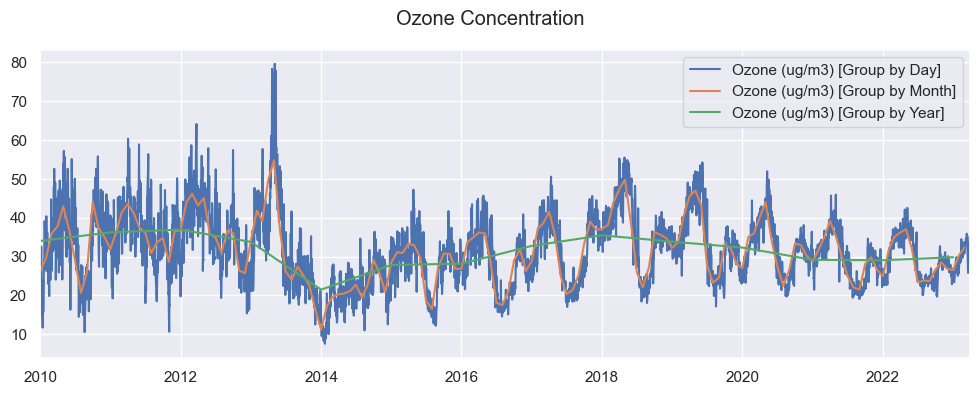
\includegraphics[width=1.0\textwidth]{img/ozone_trend_pm.png}
		\caption{Analisi dei trend giornalieri, mensili e annuali per l'Ozono.}
	\end{figure}
	\begin{figure}[H]
		\centering
		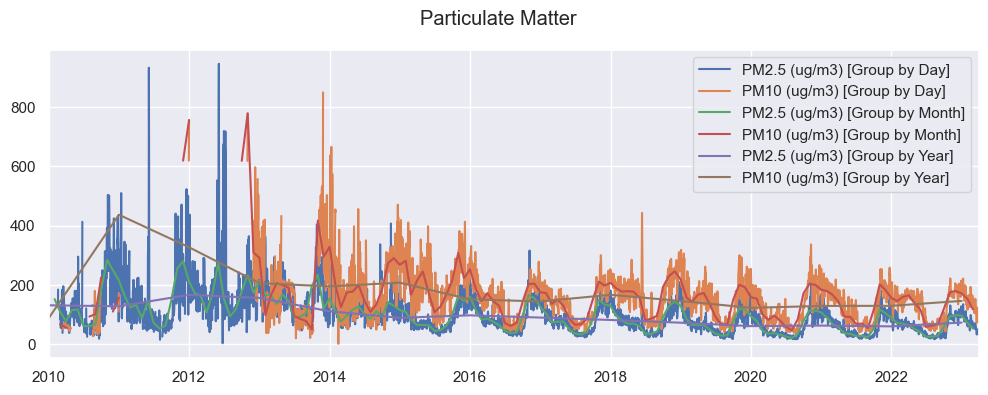
\includegraphics[width=1.0\textwidth]{img/pm_trend_pm.png}
		\caption{Analisi dei trend giornalieri, mensili e annuali per i Composti dell'azoto.}
	\end{figure}
	\begin{figure}[H]
		\centering
		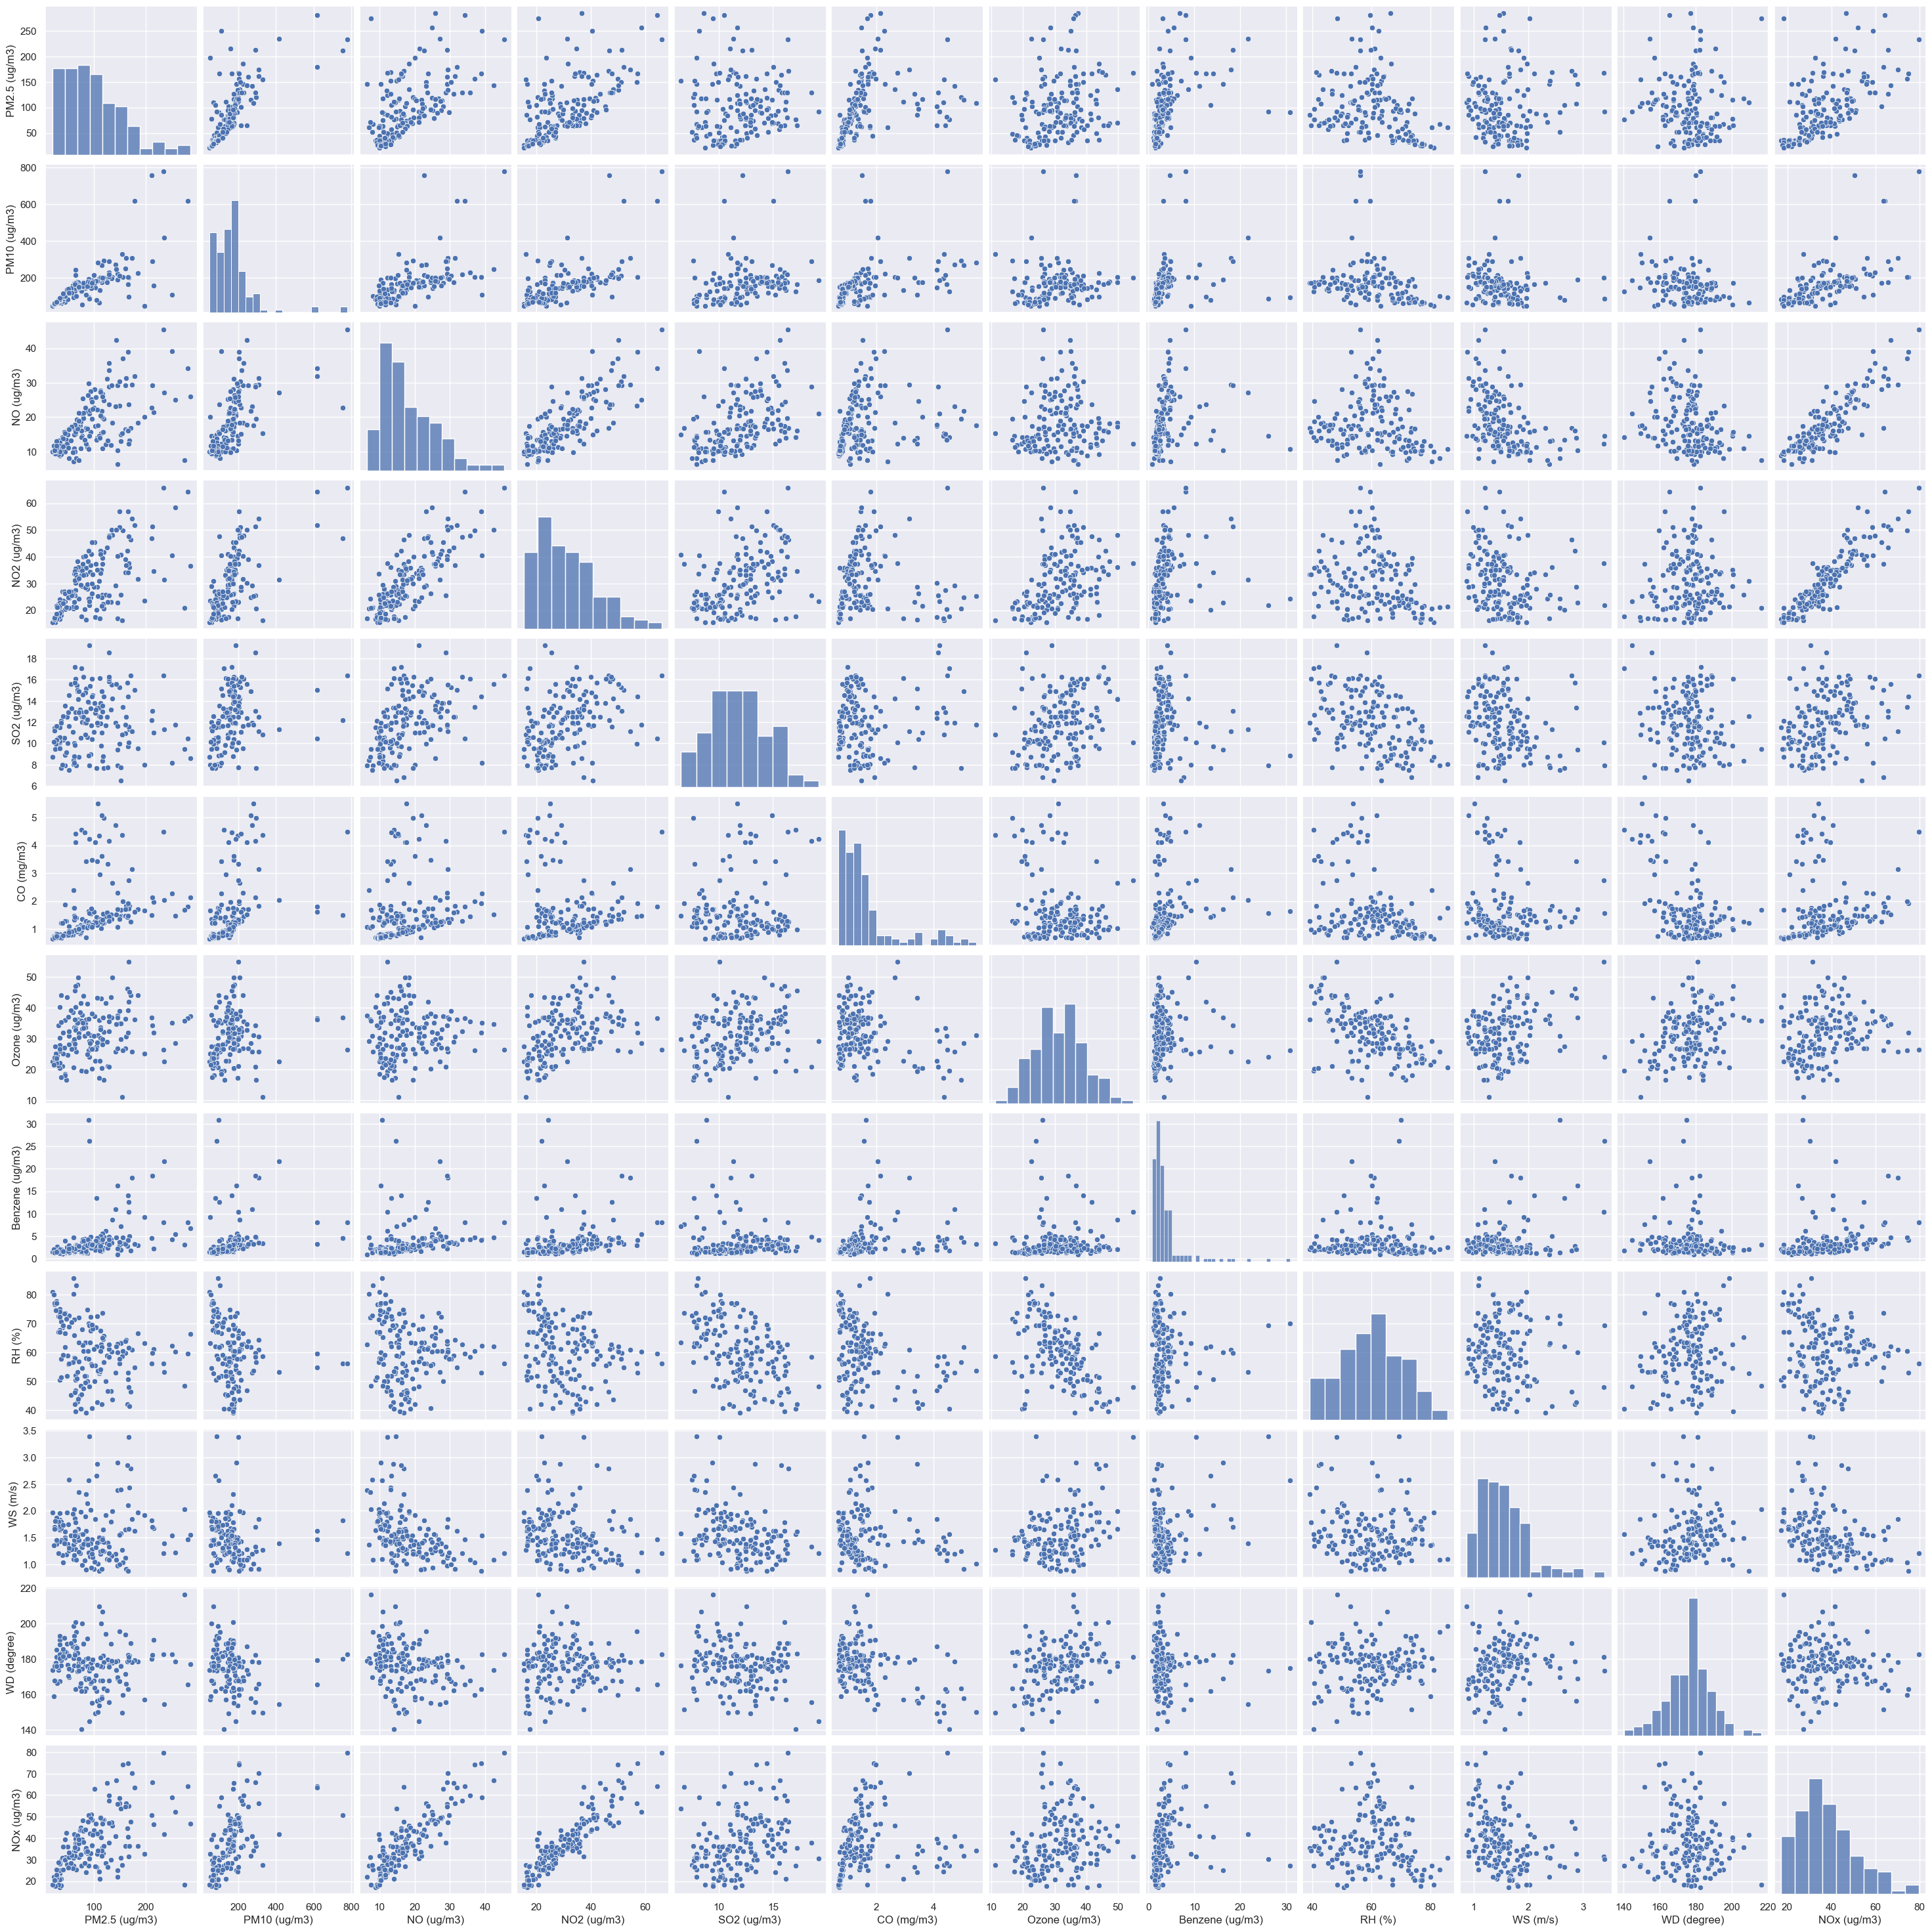
\includegraphics[width=1.0\textwidth]{img/corr_pairplot_pm.png}
		\caption{Analisi della relazione tra features e le loro distribuzioni univariate.}
	\end{figure}
	\begin{figure}[H]
		\centering
		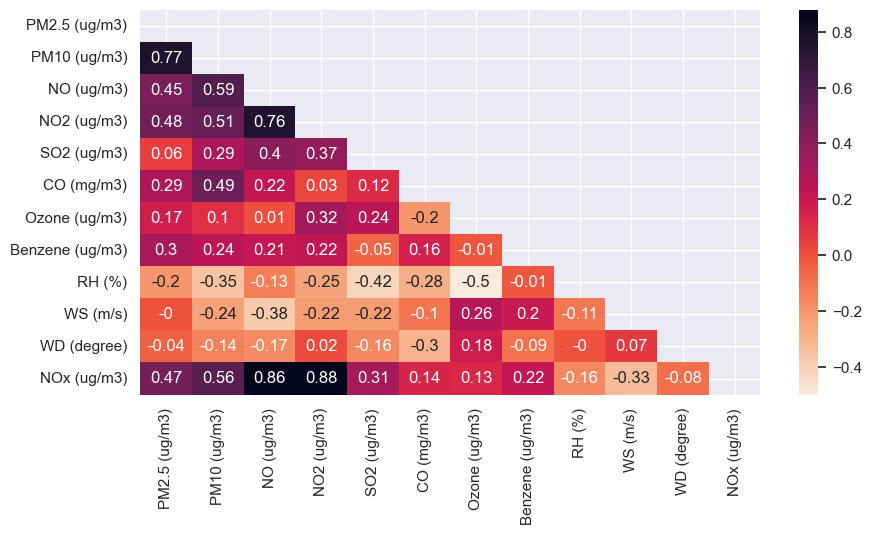
\includegraphics[width=1.0\textwidth]{img/corr_pm.png}
		\caption{Analisi della correlazione tra variabili.}
	\end{figure}
	
	Dall'analisi, si é deciso di mantenere la variabile aggregata "NOx" e rimuovere le componenti ridondanti ("NO", "NO2") per evitare multicollinearitá e semplificare i modelli successivi.
	
	\subsection{Ricampionamento ed aggregazione a livello statale}
	Poiché i dati aggregati includevano misurazioni provenienti da più stazioni all'interno dello stesso stato con lo stesso timestamp, si é deciso di ricampionare temporaneamente i dati a frequenza oraria e di aggregare le osservazioni a livello di stato tramite media aritmetica. La procedura implementata é la seguente:
	
	\begin{verbatim}
		df_resampled = df_india
			.groupby('state')
			.resample('60min')
			.mean(numeric_only=True)
			.reset_index()
	\end{verbatim}
	
	\subsection{Rilevamento e rimozione degli outlier}
	Per l'identificazione degli outlier nelle concentrazioni degli inquinanti, si è utilizzato l'algoritmo Isolation Forest, un metodo ensemble efficace per l'identificazione di valori anomali indipendentemente dalla distribuzione a priori dei dati \cite{liu2009iforest}. I punti principali dell'approccio sono stati: la scelta di un insieme limitato di variabili ("PM2.5", "CO", "Ozone", "NOx"); l'inizializzazione del modello con un valore di \texttt{contamination} pari a $0.01$ ed un \texttt{random\_state} fisso per la riproducibilità; l'addestramento del modello e l'utilizzo del metodo \texttt{predict} per etichettare le istanze anomale (-1) e quelle normali (1); infine, la rimozione delle osservazioni etichettate come outlier e la verifica della distribuzione prima e dopo tramite istogrammi.
	
	\begin{figure}[H]
		\centering
		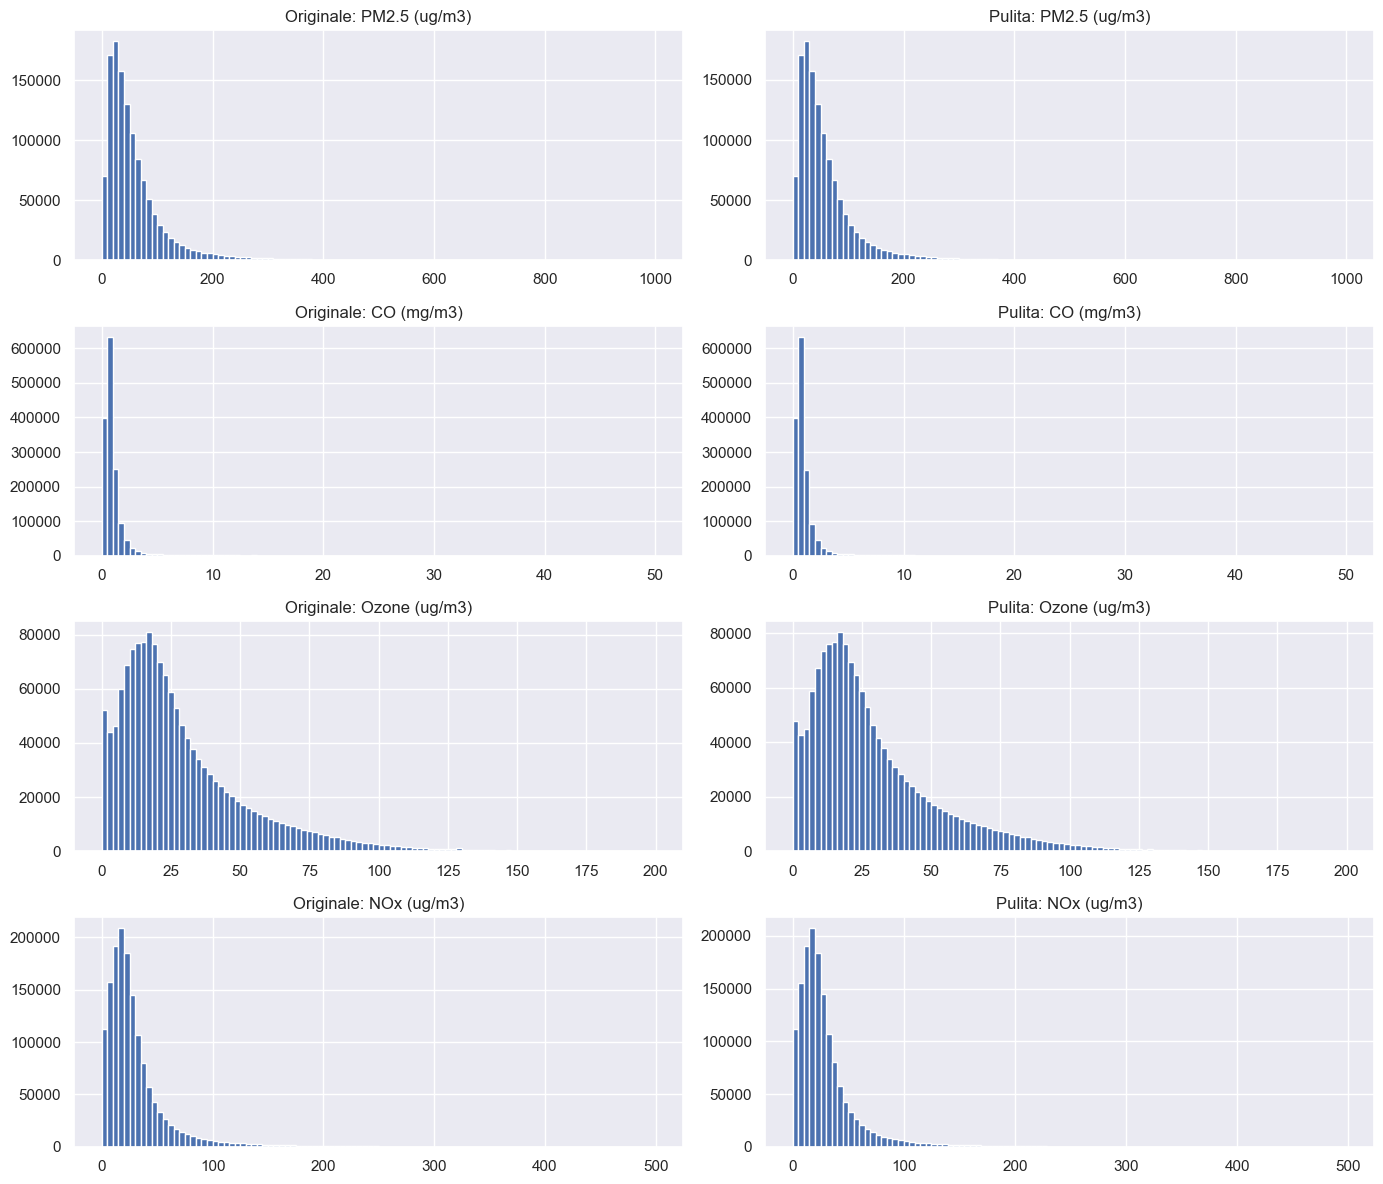
\includegraphics[width=1.0\textwidth]{img/distr_prepost_isofor_pm.png}
		\caption{Visualizzazione della distribuzione, di ogni variabile esaminata, prima e dopo.}
	\end{figure}
	
	\subsection{Feature engineering ed arricchimento temporale}
	Per catturare informazioni temporali rilevanti per aiutare i modelli a predire in modo più accurato, sono state create variabili derivate dall'indice temporale quali: "hour", "dayofmonth", "dayofweek", "dayofyear", "weekofyear", "month", "quarter" e "year". Queste variabili servono a modellare stagionalità, ciclicità giornaliera e pattern settimanali/annuali tipici dei fenomeni atmosferici e delle attività umane legate all'inquinamento atmosferico.
	
	\begin{figure}[H]
		\centering
		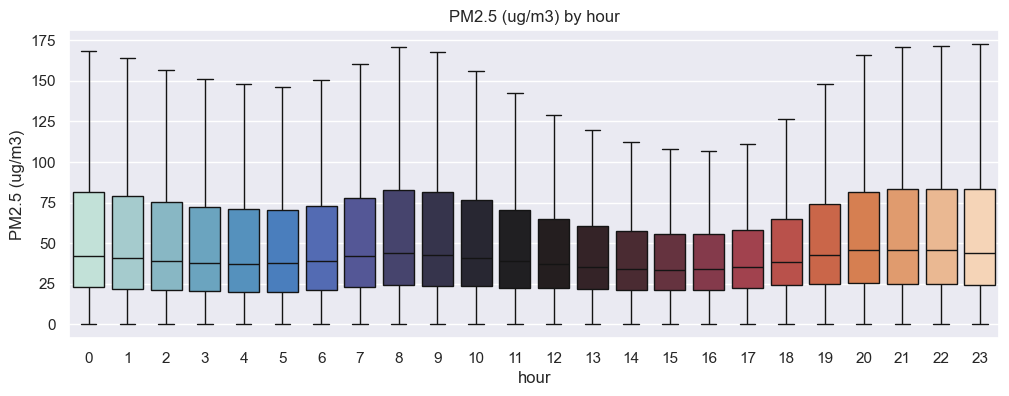
\includegraphics[width=1.0\textwidth]{img/byhour_pm.png}
		\caption{Visualizzazione della distribuzione di PM2.5 per ora.}
	\end{figure}
	\begin{figure}[H]
		\centering
		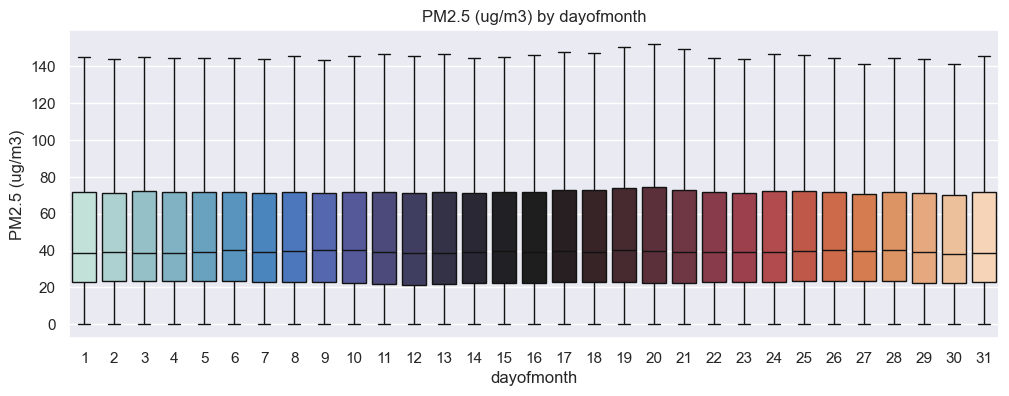
\includegraphics[width=1.0\textwidth]{img/bydayofmonth_pm.png}
		\caption{Visualizzazione della distribuzione di PM2.5 per giorno del mese.}
	\end{figure}
	\begin{figure}[H]
		\centering
		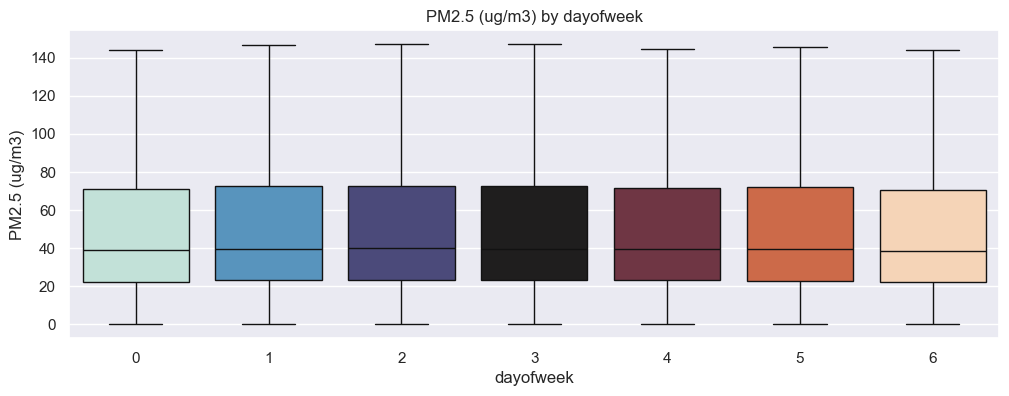
\includegraphics[width=1.0\textwidth]{img/bydayofweek_pm.png}
		\caption{Visualizzazione della distribuzione di PM2.5 per giorno della settimana.}
	\end{figure}
	\begin{figure}[H]
		\centering
		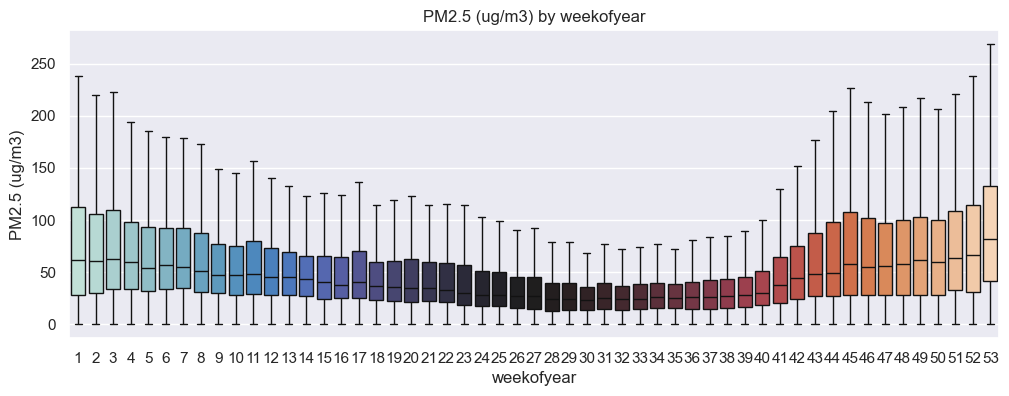
\includegraphics[width=1.0\textwidth]{img/byweekofyear_pm.png}
		\caption{Visualizzazione della distribuzione di PM2.5 per settimana dell'anno.}
	\end{figure}
	\begin{figure}[H]
		\centering
		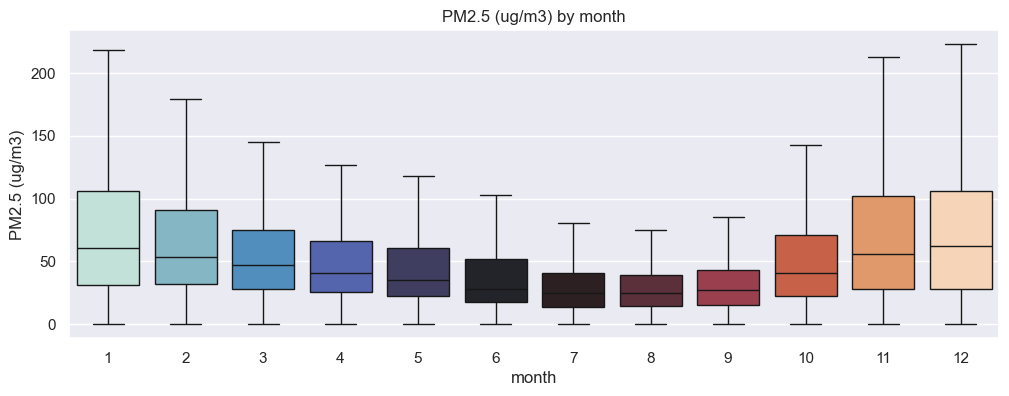
\includegraphics[width=1.0\textwidth]{img/bymonth_pm.png}
		\caption{Visualizzazione della distribuzione di PM2.5 per mese dell'anno.}
	\end{figure}
	\begin{figure}[H]
		\centering
		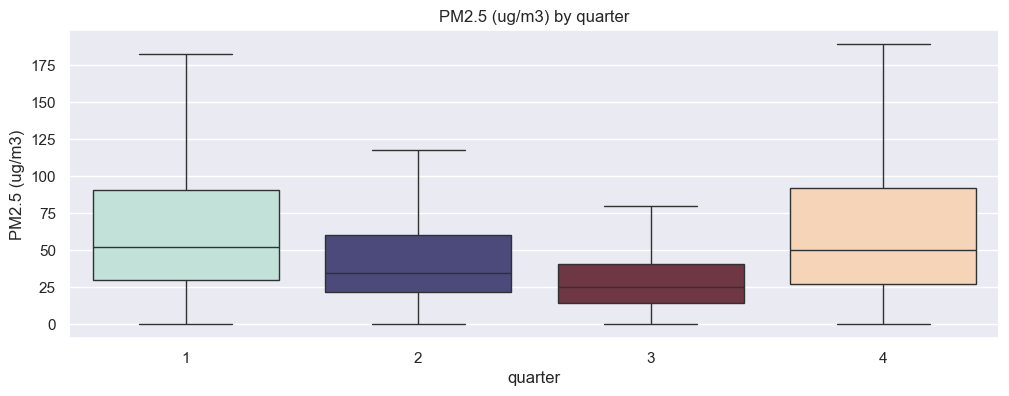
\includegraphics[width=1.0\textwidth]{img/byquarter_pm.png}
		\caption{Visualizzazione della distribuzione di PM2.5 per trimestre dell'anno.}
	\end{figure}
	\begin{figure}[H]
		\centering
		\includegraphics[width=1.0\textwidth]{img/byyear_pm.png}
		\caption{Visualizzazione della distribuzione di PM2.5 per anno.}
	\end{figure}
	
	\subsection{Creazione di lag-features e categorizzazione di PM2.5}
	
	Per catturare l'informazione storica intrinseca nelle serie temporali, sono state create delle lag-features per alcune delle variabili più rilevanti, che consentono ai modelli di sfruttare dipendenze temporali (ad esempio stagionalità annua, effetto di breve periodo (giorni/settimane) e persistenti condizioni mensili) e rappresentano una tecnica consolidata nella preparazione dei dati per serie temporali. In questo caso, sono state generate lag a lungo termine (1 e 2 anni), a medio termine (1 mese) ed a breve termine (1 settimana e ultimi 3 giorni). \\
	Per trasformare la variabile target "PM2.5" da continua a discreta, con l'obiettivo di passare da un problema di regressione ad uno di classificazione, si é deciso di mappare i valori di PM2.5 in sei categorie dell'AQI (Good, Moderate, Unhealthy for Sensitive, Unhealthy, Very Unhealthy, Hazardous) usando le soglie standard corrispondenti ai breakpoints AQI per "PM2.5" (National Ambient Air Quality Standards for PM). Questo passaggio è motivato dalla volontà di concentrarsi sulla valutazione della qualità dell'aria in termini di rischio per la salute, piuttosto che sulla semplice previsione del valore esatto della concentrazione. Per molte applicazioni, è più utile sapere se la qualità dell'aria rientra in una categoria di rischio "pericoloso" o "buono", piuttosto che prevedere un valore numerico preciso, che potrebbe non essere immediatamente interpretabile.\\
	Le soglie utilizzate, misurate in $\mu g/m^3$, sono le seguenti:
	\begin{itemize}
		\item \textbf{GOOD:} 0-9.0
		\item \textbf{MODERATE:} 9.1-35.4
		\item \textbf{UNHEALTHY FOR SENSITIVE:} 35.5-55.4
		\item \textbf{UNHEALTHY:} 55.5-125.4
		\item \textbf{VERY UNHEALTHY:} 125.5-225.4
		\item \textbf{HAZARDOUS:} 225.5+
	\end{itemize}
	Per facilitare l'analisi e l'addestramento dei modelli, le categorie sono state convertite in etichette intere da 1 (GOOD) a 6 (HAZARDOUS). Questo approccio non solo semplifica la gestione dei dati, ma mantiene anche la relazione ordinale tra le classi.
	
	\section{Addestramento dei modelli}
	
	Il dataset finale comprende le seguenti features:
	\begin{itemize}
		\item \texttt{Year}: anno della misurazione (numerica);
		\item \texttt{Month}: mese dell’anno (numerica);
		\item \texttt{DayOfMonth}: giorno del mese (numerica);
		\item \texttt{DayOfWeek}: giorno della settimana (numerica);
		\item \texttt{DayOfYear}: giorno dell’anno (numerica);
		\item \texttt{WeekOfYear}: settimana dell’anno (numerica);
		\item \texttt{Quarter}: trimestre dell’anno (numerica);
		\item \texttt{State}: stato di misurazione (categorica);
		\item \texttt{PM\_lag\_1D}, \texttt{PM\_lag\_2D}, \texttt{PM\_lag\_3D}, \texttt{PM\_lag\_1W}, \texttt{PM\_lag\_1M}, \texttt{PM\_lag\_1Y}: valori ritardati di PM2.5 rispettivamente di 1, 2, 3 giorni, 1 settimana, 1 mese e 1 anno (numeriche);
		\item \texttt{CO\_lag\_1D}, \texttt{CO\_lag\_2D}, \texttt{CO\_lag\_3D}, \texttt{CO\_lag\_1W}, \texttt{CO\_lag\_1M}, \texttt{CO\_lag\_1Y}: valori ritardati di CO rispettivamente di 1, 2, 3 giorni, 1 settimana, 1 mese e 1 anno (numeriche);
		\item \texttt{O3\_lag\_1D}, \texttt{O3\_lag\_2D}, \texttt{O3\_lag\_3D}, \texttt{O3\_lag\_1W}, \texttt{O3\_lag\_1M}, \texttt{O3\_lag\_1Y}: valori ritardati di O\textsubscript{3} rispettivamente di 1, 2, 3 giorni, 1 settimana, 1 mese e 1 anno (numeriche).
	\end{itemize}
	
	La variabile target da prevedere è una variabile discreta a 6 classi, corrispondenti ai livelli di qualità dell’aria per la concentrazione di PM2.5 definiti dalla scala \textit{EPA} (Environmental Protection Agency, USA).
	
	\subsection{Strategia di training comune e griglie di iperparametri}
	La strategia di training adottata è sostanzialmente omogenea per tutti i modelli considerati, con alcune specificità legate all'architettura di ciascun modello. Per la Random Search, il numero di iterazioni $n$ è stato scelto con una logica probabilistica per assicurare una probabilità del 90\% di includere almeno una delle 10 migliori configurazioni. Per le reti neurali (MLP e KAN), l'addestramento è stato gestito con l'ottimizzatore Adam, la funzione di perdita CrossEntropyLoss (che richiede etichette 0-indexed) ed una regolarizzazione L2 opzionale. La dimensione del batch è fissata a 32 ed il calcolo viene eseguito su GPU, se disponibile. Per evitare l'overfitting, è stato implementato un sistema di early stopping con parametri configurabili (\texttt{patience} e \texttt{min\_delta}). Inoltre, la funzione di attivazione della MLP é la ReLU. \\
	
	Di seguito sono riportate le griglie di iperparametri entro cui la Random Search esplora le combinazioni, al fine di individuare quelle che forniscono i risultati migliori per ciascun modello.
	\smallskip
	\noindent\textbf{Random Forest} \quad (Random Search: $n=49$)
	\begin{itemize}
		\item \texttt{n\_estimators}: [100, 150, 200]
		\item \texttt{max\_samples}: [0.5, 0.7, 0.9]
		\item \texttt{max\_depth}: [5, 10, 15]
		\item \texttt{min\_samples\_split}: [2, 5]
		\item \texttt{min\_samples\_leaf}: [2, 5]
		\item \texttt{max\_features}: ['sqrt', 'log2']
	\end{itemize}
	
	\smallskip
	\noindent\textbf{XGBoost} \quad (Random Search: $n=98$)
	\begin{itemize}
		\item \texttt{max\_depth}: [3, 5]
		\item \texttt{learning\_rate}: [0.01, 0.05, 0.1]
		\item \texttt{n\_estimators}: [100, 200, 300]
		\item \texttt{subsample}: [0.7, 0.9]
		\item \texttt{colsample\_bytree}: [0.7, 0.9]
		\item \texttt{gamma}: [0, 0.2, 0.4]
		\item \texttt{min\_child\_weight}: [1, 5]
	\end{itemize}
	
	\smallskip
	\noindent\textbf{MLP} \quad (Random Search: $n=26$)
	\begin{itemize}
		\item \texttt{hidden\_sizes}: [(64,64), (128,), (128,64), (256,128), (512,256)];
		\item \texttt{dropout}: [0.0, 0.2, 0.5];
		\item \texttt{lr} (learning rate): [$10^{-3}$, $10^{-4}$];
		\item \texttt{l2\_lambda} (coefficiente L2): [0.0, $10^{-5}$, $10^{-4}$, $10^{-3}$].
	\end{itemize}
	
	\smallskip
	\noindent\textbf{KAN} \quad (Random Search: $n=43$)
	\begin{itemize}
		\item \texttt{width}: [(8,4), (16,8), (32,16), (64,32)] (struttura a livelli della rete);
		\item \texttt{grid}: [5, 10, 20] (dimensione della griglia interna);
		\item \texttt{k}: [2, 4] (ordine/complessit\`a della combinazione);
		\item \texttt{seed}: [0] (per riproducibilit\`a);
		\item \texttt{lr}: [$10^{-3}$, $10^{-4}$];
		\item \texttt{l2\_lambda}: [0.0, $10^{-3}$, $10^{-4}$, $10^{-5}$].
	\end{itemize}
	
	\subsection{Scelte architetturali finali}
	Nella Tabella \ref{tab:model-config-pm} vengono mostrate le scelte finali, dopo l'ottimizzazione degli iperparametri, utilizzate per training, valutazioni comparative e studio di ablazione.
	
	\begin{table}[H]
		\centering
		\caption{Configurazioni finali dei modelli usati per il Training, dopo aver effettuato l'ottimizzazione degli iperparametri.}
		\label{tab:model-config-pm}
		\begin{tabular}{l p{0.65\linewidth}}
			\toprule
			\textbf{MLP} & \texttt{input\_dim = 49}; \texttt{hidden\_sizes = (64, 64)}; \texttt{dropout = 0.2}; \texttt{ottimizzatore = Adam}; \texttt{lr = 1e-04}; \texttt{l2\_lambda = 1e-03}; \texttt{batch\_size = 32}. Early stopping applicato. \\
			\midrule
			\textbf{KAN} & \texttt{input\_dim = 49}; \texttt{width = (16,8)}; \texttt{grid = 5}; \texttt{k = 4}, \texttt{seed = 0}; \texttt{ottimizzatore = Adam}; \texttt{lr = 1e-04}; \texttt{l2\_lambda = 1e-05}; \texttt{batch\_size = 32}. Early stopping applicato. \\
			\midrule
			\textbf{Random Forest} & \texttt{n\_estimators = 100}; \texttt{max\_depth = 15}; \texttt{min\_samples\_split = 5}; \texttt{min\_samples\_leaf = 2}; \texttt{max\_features = 'sqrt'}; \texttt{max\_samples = 0.7}; \texttt{random\_state = 42}. \\
			\midrule
			\textbf{XGBoost} & \texttt{n\_estimators = 300}; \texttt{max\_depth = 5}; \texttt{learning\_rate = 0.05}; \texttt{subsample = 0.9}; \texttt{colsample\_bytree = 0.7}; \texttt{min\_child\_weight = 1}; \texttt{gamma = 0.2}; \texttt{objective = 'multi:softprob'}; \texttt{eval\_metric = 'mlogloss'}; \texttt{random\_state = 42}. \\
			\bottomrule
		\end{tabular}
	\end{table}
	
	\section{Valutazione dei modelli}
	
	La figura \ref{fig:comparison_pm} sintetizza le principali metriche di performance (Accuracy, F1-weighted, F1-macro, AUC-ROC e AUC-PR) con intervalli di confidenza al 95\% (bootstrap) e la complessitá dei modelli.
	
	\begin{figure}[H]
		\centering
		\includegraphics[width=1.0\textwidth]{img/comparison_pm.png}
		\caption{Confronto visivo delle prestazioni dei modelli (Accuracy train vs test, F1-weighted / F1-macro con CI95\%, AUC-ROC e AUC-PR OVR weighted, e complessità in parametri/nodi).}
		\label{fig:comparison_pm}
	\end{figure}
	
	\subsubsection{Classification report e confusion matrix per modello}
	
	\paragraph{Random Forest} \mbox{}\\
	Numero di parametri / nodi: \textbf{412\,430}.
	
	\begin{table}[H]
		\centering
		\caption{Classification report}
		\label{tab:cr_rf}
		\begin{tabular}{lrrrr}
			\toprule
			Classe & precision & recall & f1-score & support \\
			\midrule
			0 & 0.76 & 0.73 & 0.74 & 321 \\
			1 & 0.89 & 0.86 & 0.88 & 2\,727 \\
			2 & 0.65 & 0.70 & 0.67 & 1\,364 \\
			3 & 0.85 & 0.80 & 0.82 & 1\,831 \\
			4 & 0.61 & 0.82 & 0.70 & 307 \\
			5 & 0.32 & 0.37 & 0.34 & 30 \\
			\midrule
			accuracy & \multicolumn{3}{c}{0.80} & 6\,580 \\
			macro avg & 0.68 & 0.71 & 0.69 & 6\,580 \\
			weighted avg & 0.81 & 0.80 & 0.80 & 6\,580 \\
			\bottomrule
		\end{tabular}
	\end{table}
	
	\begin{table}[H]
		\centering
		\caption{Confusion matrix}
		\label{tab:cm_rf}
		\[
		\begin{bmatrix}
			233 & 88  & 0   & 0   & 0   & 0   \\
			73  & 2350& 286 & 18  & 0   & 0   \\
			1   & 196 & 953 & 213 & 1   & 0   \\
			0   & 9   & 222 & 1456& 143 & 1   \\
			0   & 1   & 0   & 32  & 252 & 22  \\
			0   & 0   & 0   & 0   & 19  & 11
		\end{bmatrix}
		\]
		\vspace{1mm}
		
		AUC-ROC (OVR, weighted): \textbf{0.952} \\
		AUC-PR  (OVR, weighted): \textbf{0.858}
	\end{table}
	
	
	\paragraph{XGBoost} \mbox{}\\
	Numero di parametri / nodi: \textbf{90\,416}.
	
	\begin{table}[H]
		\centering
		\caption{Classification report}
		\label{tab:cr_xgb}
		\begin{tabular}{lrrrr}
			\toprule
			Classe & precision & recall & f1-score & support \\
			\midrule
			0 & 0.76 & 0.79 & 0.77 & 321 \\
			1 & 0.89 & 0.87 & 0.88 & 2\,727 \\
			2 & 0.67 & 0.68 & 0.68 & 1\,364 \\
			3 & 0.83 & 0.85 & 0.84 & 1\,831 \\
			4 & 0.69 & 0.70 & 0.70 & 307 \\
			5 & 0.32 & 0.43 & 0.37 & 30 \\
			\midrule
			accuracy & \multicolumn{3}{c}{0.81} & 6\,580 \\
			macro avg & 0.69 & 0.72 & 0.71 & 6\,580 \\
			weighted avg & 0.81 & 0.81 & 0.81 & 6\,580 \\
			\bottomrule
		\end{tabular}
	\end{table}
	
	\begin{table}[H]
		\centering
		\caption{Confusion matrix}
		\label{tab:cm_xgb}
		\[
		\begin{bmatrix}
			253 & 68  & 0   & 0   & 0   & 0   \\
			79  & 2360& 266 & 22  & 0   & 0   \\
			1   & 200 & 930 & 232 & 1   & 0   \\
			0   & 8   & 187 & 1556& 78  & 2   \\
			0   & 1   & 0   & 64  & 216 & 26  \\
			0   & 0   & 0   & 0   & 17  & 13
		\end{bmatrix}
		\]
		\vspace{1mm}
		
		AUC-ROC (OVR, weighted): \textbf{0.957} \\
		AUC-PR  (OVR, weighted): \textbf{0.875}
	\end{table}
	
	
	\paragraph{MLP} \mbox{}\\
	Numero di parametri: \textbf{7\,750}.
	
	\begin{table}[H]
		\centering
		\caption{Classification report}
		\label{tab:cr_mlp}
		\begin{tabular}{lrrrr}
			\toprule
			Classe & precision & recall & f1-score & support \\
			\midrule
			0 & 0.43 & 0.38 & 0.40 & 321 \\
			1 & 0.86 & 0.80 & 0.83 & 2\,727 \\
			2 & 0.63 & 0.72 & 0.67 & 1\,364 \\
			3 & 0.85 & 0.80 & 0.82 & 1\,831 \\
			4 & 0.59 & 0.82 & 0.69 & 307 \\
			5 & 0.37 & 0.57 & 0.45 & 30 \\
			\midrule
			accuracy & \multicolumn{3}{c}{0.76} & 6\,580 \\
			macro avg & 0.62 & 0.68 & 0.64 & 6\,580 \\
			weighted avg & 0.77 & 0.76 & 0.77 & 6\,580 \\
			\bottomrule
		\end{tabular}
	\end{table}
	
	\begin{table}[H]
		\centering
		\caption{Confusion matrix}
		\label{tab:cm_mlp}
		\[
		\begin{bmatrix}
			121 & 200 & 0   & 0   & 0   & 0   \\
			157 & 2189& 360 & 21  & 0   & 0   \\
			4   & 160 & 977 & 220 & 3   & 0   \\
			0   & 5   & 204 & 1465& 156 & 1   \\
			0   & 1   & 0   & 27  & 251 & 28  \\
			0   & 0   & 0   & 0   & 13  & 17
		\end{bmatrix}
		\]
		\vspace{1mm}
		
		AUC-ROC (OVR, weighted): \textbf{0.938} \\
		AUC-PR  (OVR, weighted): \textbf{0.800}
	\end{table}
	
	
	\paragraph{KAN} \mbox{}\\
	Numero di parametri: \textbf{7\,680}.
	
	\begin{table}[H]
		\centering
		\caption{Classification report}
		\label{tab:cr_kan}
		\begin{tabular}{lrrrr}
			\toprule
			Classe & precision & recall & f1-score & support \\
			\midrule
			0 & 0.65 & 0.36 & 0.46 & 321 \\
			1 & 0.85 & 0.85 & 0.85 & 2\,727 \\
			2 & 0.63 & 0.72 & 0.67 & 1\,364 \\
			3 & 0.84 & 0.82 & 0.83 & 1\,831 \\
			4 & 0.74 & 0.69 & 0.71 & 307 \\
			5 & 0.51 & 0.60 & 0.55 & 30 \\
			\midrule
			accuracy & \multicolumn{3}{c}{0.78} & 6\,580 \\
			macro avg & 0.70 & 0.67 & 0.68 & 6\,580 \\
			weighted avg & 0.79 & 0.78 & 0.78 & 6\,580 \\
			\bottomrule
		\end{tabular}
	\end{table}
	
	\begin{table}[H]
		\centering
		\caption{Confusion matrix}
		\label{tab:cm_kan}
		\[
		\begin{bmatrix}
			116 & 204 & 1   & 0   & 0   & 0   \\
			61  & 2329& 320 & 17  & 0   & 0   \\
			2   & 198 & 985 & 179 & 0   & 0   \\
			0   & 7   & 261 & 1498& 63  & 2   \\
			0   & 1   & 0   & 79  & 212 & 15  \\
			0   & 0   & 0   & 0   & 12  & 18
		\end{bmatrix}
		\]
		\vspace{1mm}
		
		AUC-ROC (OVR, weighted): \textbf{0.948} \\
		AUC-PR  (OVR, weighted): \textbf{0.840}
	\end{table}
	
	\subsection{Risultati sperimentali}
	
	L'analisi dei classification report e delle confusion matrix (riportati nella sottosezione precedente) mostra che, a livello di metriche aggregate, le differenze tra i modelli testati sono complessivamente contenute: accuratezza, F1-score, AUC-ROC e AUC-PR si collocano su valori molto simili, con scarti percentuali spesso marginali. La discriminante più evidente è la complessità architetturale, che diventa il fattore operativo principale per decisioni di deployment, latenza e consumo di memoria. \\ 
	Per quanto riguarda le reti neurali, la \textbf{MLP} ha ottenuto un'accuratezza in test pari al $76\%$, con un F1-weighted di $0.7654$, un F1-macro di $0.7421$, un AUC-ROC di $0.938$ e un AUC-PR di $0.800$. L'analisi per classe evidenzia una sensibilità ridotta sulle classi meno rappresentate (ad es. la classe \texttt{0} è spesso confusa), sebbene il modello mantenga buone prestazioni sulla classe maggioritaria (\texttt{1}). Con circa $7{,}750$ parametri la MLP è una soluzione leggera e facilmente scalabile, ma meno competitiva rispetto ad altre alternative sul piano delle performance complessive. \\ 
	La \textbf{KAN} ha mostrato un comportamento più equilibrato: accuratezza in test del $78\%$, F1-weighted $0.7823$, F1-macro $0.7608$, AUC-ROC $0.948$ e AUC-PR $0.840$. KAN presenta inoltre una migliore capacità di trattare le classi meno rappresentate rispetto alla MLP (si osservano recall e F1 mediamente più alti su alcune classi difficili), mantenendo un numero di parametri molto contenuto (circa $7{,}680$). Queste caratteristiche rendono KAN una candidata interessante quando si richiede un buon compromesso tra accuratezza e parsimonia computazionale. \\ 
	I modelli ensemble si differenziano principalmente per il trade-off tra performance leggermente migliori e complessità superiore. La \textbf{Random Forest}, con circa $412$k nodi, ha raggiunto un'accuratezza dell'$80\%$, F1-weighted $0.7997$, F1-macro $0.7750$, AUC-ROC $0.952$ e AUC-PR $0.858$. Le confusion matrix mostrano che Random Forest è robusta nel predire la classe maggioritaria e riduce alcune specifiche confusioni osservate nelle reti neurali, ma il costo in termini di complessità è molto elevato. \\ 
	\textbf{XGBoost} è risultato il modello con le metriche aggregate più alte: accuratezza in test $81\%$, F1-weighted $0.8107$, F1-macro $0.7901$, AUC-ROC $0.957$ e AUC-PR $0.875$. Tuttavia i miglioramenti rispetto a KAN e Random Forest sono marginali. Con circa $90$k parametri XGBoost occupa una posizione intermedia: molto più leggero della Random Forest ma sensibilmente più complesso rispetto alle architetture neurali leggere come MLP e KAN. Dal confronto delle confusion matrix emerge come XGBoost migliori leggermente il recall sulle classi meno rappresentate rispetto a Random Forest e MLP, pur restando i guadagni contenuti in termini assoluti. \\
	Va inoltre segnalato che, per mitigare lo sbilanciamento delle classi, nel training sono state impiegate sia la ponderazione degli errori per classe (class weights) sia una procedura di oversampling basata su SMOTE. Queste contromisure hanno portato a miglioramenti locali nei punteggi di recall sulle classi minority (riducendo alcuni falsi negativi), ma non hanno eliminato completamente le difficoltà associate alle classi con supporto molto basso.
	
	\subsection{Selezione del miglior modello}
	Per identificare il modello più adatto al problema di classificazione, è stata adottata una procedura di ranking multi-criterio che combina le prestazioni con la complessità. Inizialmente, sono state definite le metriche di interesse e la rispettiva direzione di ottimizzazione, come indicato nel seguente blocco di codice:
	
	\begin{verbatim}
		metrics = {
			'Accuracy_Test': 'max',
			'F1_Weighted_Test': 'max',
			'F1_Macro_Test': 'max',
			'AUC_ROC_OVR_Weighted': 'max',
			'AUC_PR_OVR_Weighted': 'max'
		}
	\end{verbatim}
	
	Per ciascuna metrica, è stato calcolato il "rank" dei modelli (rank 1 = migliore). Successivamente, un performance\_score è stato calcolato come media dei rank di prestazione, mentre un Complexity\_rank è stato determinato in base al numero di parametri/nodi (rank 1 = meno complesso). Infine, performance e complessità sono state combinate attraverso diverse strategie di ponderazione: Equal Weight (1:1), dato dalla somma di performance\_score e Complexity\_rank; Complexity Weighted (1:2), che attribuisce un peso doppio alla complessità; Extreme Complexity (1:3), con un peso triplo; e il Pareto Approach (40:60), che normalizza i punteggi e li combina con pesi di 0.4 per la performance e 0.6 per la complessità. Per ogni metodo, è stato scelto il modello con il punteggio più basso. \\
	I risultati di questa procedura di ranking mostrano che XGBoost è il migliore secondo i criteri di Equal Weight (1:1) e Pareto Approach (40:60), mentre la MLP risulta vincente nei criteri Complexity Weighted (1:2) ed Extreme Complexity (1:3). I valori principali utilizzati per il ranking sono riassunti nella tabella seguente:
	
	\begin{table}[H]
		\centering
		\setlength{\tabcolsep}{6pt}
		\caption{Riepilogo ranking aggiornato: conteggio parametri, performance media (rank-based) e ranks per metodo di aggregazione.}
		\begin{tabular}{lrrrrrr}
			\toprule
			\textbf{Model} & \textbf{Param\_Count} & \textbf{Avg\_Perf} & \textbf{Compl\_Rank} & \textbf{Equal\_Rank} & \textbf{Ext\_Rank} & \textbf{Pareto\_Rank} \\
			\midrule
			KAN           & 7,680    & 3.0 & 1 & 1 & 1 & 1 \\
			xgboost       & 90,416   & 1.0 & 2 & 1 & 2 & 2 \\
			MLP           & 7,750    & 4.0 & 3 & 3 & 2 & 3 \\
			random\_forest& 412,430  & 2.0 & 4 & 3 & 4 & 4 \\
			\bottomrule
		\end{tabular}
	\end{table}
	
	\subsubsection{Conclusioni}
	Dalla procedura di ranking multi-criterio, XGBoost presenta le performance assolute più elevate sulle metriche di classificazione (in particolare l'F1-weighted), ma richiede una complessità molto maggiore rispetto alle reti neurali testate. KAN offre un eccellente compromesso fra accuratezza e parsimonia e, nelle strategie che penalizzano la complessità, risulta il modello raccomandato per il deployment. La MLP mantiene un buon rapporto performance/complessità, ma è lievemente inferiore a KAN, secondo il criterio complexity-weighted. Il Random Forest, pur competitivo in termini di metriche assolute, è meno interessante quando la parsimonia del modello è un vincolo operativo. \\
	La classifica dei tre migliori modelli, basata sul criterio "complexity-weighted" (dal migliore al peggiore), è la seguente:
	\begin{enumerate}
		\item KAN \quad (Params: 7,680 \;|\; F1-Weighted: 0.7823)
		\item xgboost \quad (Params: 90,416 \;|\; F1-Weighted: 0.8107)
		\item MLP \quad (Params: 7,750 \;|\; F1-Weighted: 0.7654)
	\end{enumerate}
	
	\section{Studio di ablazione}
	
	\subsection{Ablation study: L1 pruning su MLP e KAN}
	L'obiettivo è misurare il compromesso tra compressione del modello (numero di parametri attivi / rapporto di compressione) e il mantenimento delle prestazioni (Accuracy, F1, AUC).
	
	\subsubsection{Metodologia}
	La tecnica di pruning impiegata è il L1 post-training pruning, applicato ai pesi lineari della MLP ed ai coefficienti spline della KAN. Sono stati testati diversi pruning ratios, specificamente l'insieme ${0.0,0.1,0.2,0.3,0.4,0.5,0.6,0.7,0.8,0.9,0.95}$. Ciascuna versione del modello potata è stata valutata sia sul test set che sul train set sulle stesse metriche definite precedentemente. Per ogni configurazione, sono stati calcolati il numero totale di parametri, il numero di parametri attivi post-pruning ed il rapporto di compressione. Per interpretare i risultati, sono state definite alcune definizioni operative. La baseline è il modello non potato (pruning ratio $= 0.0$). Il punto di degrado significativo è il primo pruning ratio che comporta una perdita relativa in \texttt{F1-Weighted} superiore al 5\% rispetto alla baseline. Il best trade-off è il punto di massima compressione che causa una perdita relativa in \texttt{F1-Weighted} inferiore o uguale al 2\%.
	
	\subsubsection{Figura riassuntiva}
	\begin{figure}[H]
		\centering
		\includegraphics[width=1.0\textwidth]{img/abl_kanvsmlp_pm.png}
		\caption{Risultati dello studio L1 pruning per MLP e KAN, utilizzando metriche principali e indicatori di compressione (Accuracy, F1-Weighted, F1-Macro, AUC-ROC, AUC-PR, sparsitá, parametri attivi, performance retention).}
	\end{figure}
	
	\subsubsection{Risultati}
	\begin{table}[H]
		\centering
		\setlength{\tabcolsep}{4pt}
		\begin{tabular}{lcccc}
			\toprule
			\textbf{Model} & \textbf{Total params} & \textbf{Baseline F1} & \textbf{Best trade-off} & \textbf{Sign. degr.} \\
			\midrule
			MLP & 7,750   & 0.7654 & 50\% pruning (2.0$\times$ compression) & 70\% pruning \\
			KAN & 7,680   & 0.7823 & 70\% pruning (3.0$\times$ compression) & 90\% pruning \\
			\bottomrule
		\end{tabular}
		\caption{Riepilogo dei punti di trade-off e dei punti di degrado osservati nello studio L1 pruning (valori aggiornati).}
	\end{table}
	
	La MLP, con baseline \texttt{F1-Weighted} = \(\mathbf{0.7654}\), mostra il miglior trade-off al \(\mathbf{50\%}\) di pruning: in questa condizione la compressione è di circa \(2\times\) e la variazione relativa in F1-weighted è trascurabile (ossia \(\le 0.2\%\) in termini assoluti, nel nostro run si è misurata una variazione leggermente positiva rispetto alla baseline). Il punto di degrado significativo per la MLP si evidenzia a partire da circa il \(\mathbf{70\%}\) di pruning, oltre il quale la perdita di performance diventa marcata; a pruning estremi (\(\ge 90\%\)) le prestazioni decadono drasticamente. \\
	La KAN, con baseline \texttt{F1-Weighted} = \(\mathbf{0.7823}\), risulta più robusta per pruning moderati: il miglior trade-off osservato è al \(\mathbf{70\%}\) di pruning, corrispondente a una compressione di circa \(3\times\) e a una perdita relativa in F1-weighted dell'ordine di \(\approx 1.4\%\). La soglia di degrado significativo per KAN si trova invece intorno al \(\mathbf{90\%}\) di pruning. \\
	La compressione massima raggiungibile nei test è stata dell'ordine di $\sim 20\times$ per la MLP e $\sim 17.8\times$ per la KAN (pruning $95\%$), ma tali livelli estremi comportano perdite di prestazione troppo elevate per essere considerati praticabili in un contesto di deployment senza ulteriori tecniche (ad esempio, retraining post-pruning).
	
	\subsection{Ablation study: ensemble pruning su Random Forest e XGBoost}
	Lo scopo è valutare il compromesso tra riduzione del modello (numero di alberi / rounds) e mantenimento delle prestazioni (F1-weighted, accuracy, AUC).
	
	\subsubsection{Metodologia}
	La metodologia di pruning varia per i due modelli. Per il Random Forest, è stato utilizzato un Rank-based Pruning: gli alberi sono stati ordinati per importanza (somma delle feature importances dell'albero) e quelli meno rilevanti sono stati rimossi fino a raggiungere il \texttt{pruning\_ratio} desiderato. Per XGBoost, si è optato per un Cumulative Pruning, mantenendo solo le prime iterazioni di boosting fino al numero corrispondente a \((1 - \texttt{pruning\_ratio})\) della lunghezza originale, troncando di fatto la sequenza di boosting. Anche in questo caso, i pruning ratios testati sono stati ${0.0,0.1,0.2,0.3,0.4,0.5,0.6,0.7,0.8,0.9,0.95}$. Per ogni versione potata, sono stati calcolati il numero totale e residuo di alberi, il rapporto di compressione e le metriche di performance su train e test set. Le definizioni operative di baseline, punto di degrado significativo ($\texttt{F1-Weighted} >5\%$) e best trade-off ($\texttt{F1-Weighted} \le 2\%$) sono rimaste le medesime.
	
	\subsubsection{Figura riassuntiva}
	\begin{figure}[H]
		\centering
		\includegraphics[width=\textwidth]{img/abl_xgbvsrf_pm.png}
		\caption{Risultati dello studio di pruning per Random Forest (rank-based) e XGBoost (cumulative), utilizzando metriche principali e indicatori di compressione (Accuracy, F1-Weighted, F1-Macro, AUC-ROC, AUC-PR, sparsitá, alberi rimanenti, performance retention).}
	\end{figure}
	
	\subsubsection{Risultati}
	\begin{table}[H]
		\centering
		\setlength{\tabcolsep}{4pt}
		\begin{tabular}{lcccc}
			\toprule
			\textbf{Model} & \textbf{Total trees} & \textbf{Baseline F1} & \textbf{Best trade-off (pruning)} & \textbf{Sign. degr.} \\
			\midrule
			Random Forest & 100 & 0.8011 & 90\% (9 trees rimasti, $\approx 11.1\times$ compression) & nessuna degr. rilevata \\
			XGBoost       & 300 & 0.8107 & 60\% (120 rounds rimasti, $\approx 2.5\times$ compression) & nessuna degr. rilevata \\
			\bottomrule
		\end{tabular}
		\caption{Riepilogo sintetico dei punti di trade-off osservati per i due ensemble (valori aggiornati).}
	\end{table}
	
	XGBoost mantiene buona parte delle prestazioni riducendo il numero di rounds. Il miglior compromesso osservato nel run corrente è stato al $60\%$ di pruning, con i primi 120 rounds su 300, corrispondente a una compressione di $\approx 2.5\times$ ed ad una perdita relativa in F1-weighted di circa $1.5\%$ rispetto alla baseline. \\
	Random Forest dimostra elevata robustezza: l'approccio rank-based permette di rimuovere un gran numero di alberi mantenendo metriche stabili; nel nostro esperimento il best trade-off si è verificato al $90\%$ di pruning (9 alberi rimanenti), con una compressione $\approx 11.11\times$ ed una perdita relativa in F1-weighted di circa $1.7\%$. In nessuno dei due casi si è osservata una perdita relativa superiore al $5\%$ nell'intervallo di pruning testato. \\
	La compressione massima sperimentata è stata dell'ordine di $\sim 20\times$ per Random Forest e $\sim 25\times$ per XGBoost (pruning $95\%$), tuttavia tali livelli estremi comportano perdite di prestazione significativamente maggiori e risultano poco praticabili senza interventi aggiuntivi (es. fine-tuning post-pruning, distillazione o quantizzazione).
	
	\subsection{Ablation study — Confronto complessivo (Neural Networks vs Ensemble)}
	Per un confronto complessivo, sono stati estratti i risultati di ogni modello a soglie tipiche di pruning: 30\%, 50\%, 70\% e 90\%. Le metriche e gli output considerati includono: Accuracy (test), F1-Weighted (test), F1-Macro (test), AUC-ROC e AUC-PR weighted (quando calcolabili), il rapporto di compressione e le statistiche di performance retention (pruned/baseline).
	
	\subsubsection{Figure riassuntive}
	\begin{figure}[H]
		\centering
		\begin{minipage}{0.49\textwidth}
			\centering
			\includegraphics[width=\linewidth]{img/abl_kanvsmlp_pm.png}
			\caption*{A: Studio di ablazione MLP e KAN (L1 pruning).}
		\end{minipage}\hfill
		\begin{minipage}{0.49\textwidth}
			\centering
			\includegraphics[width=\linewidth]{img/abl_xgbvsrf_pm.png}
			\caption*{B: Studio di ablazione Random Forest (rank-based) e XGBoost (cumulative).}
		\end{minipage}
		\caption{Risultati sintetici degli studi di ablazione.}
	\end{figure}
	
	\subsubsection{Riepilogo}
	\begin{table}[H]
		\centering
		\begin{tabular}{lccc}
			\toprule
			\textbf{Model} & \textbf{Baseline F1 (weighted)} & \textbf{Best trade-off (pruning)} & \textbf{Compression} \\
			\midrule
			MLP      & 0.7654 & 0.7662 @ 50\% pr & $\approx 2.0\times$ \\
			KAN      & 0.7823 & 0.7710 @ 70\% pr & $\approx 3.0\times$ \\
			RF       & 0.8011 & 0.7878 @ 90\% pr & $\approx 11.1\times$ \\
			XGBoost  & 0.8107 & 0.7982 @ 60\% pr & $\approx 2.5\times$ \\
			\bottomrule
		\end{tabular}
		\caption{Riepilogo sintetico dei principali punti di trade-off e compressione (valori aggiornati).}
	\end{table}
	
	Al 30\% di pruning, tutti i modelli mantengono o presentano leggeri miglioramenti rispetto alla baseline nelle metriche principali: MLP mostra un lieve incremento dell'F1-weighted, mentre KAN e XGBoost mantengono prestazioni molto elevate. A 50\% di pruning la MLP raggiunge il suo miglior trade-off operativo (compressione $\sim 2\times$ con F1-weighted sostanzialmente invariata rispetto alla baseline), mentre KAN e gli ensemble rimangono stabili. A 70\% di pruning XGBoost continua a mostrare una ritenzione delle prestazioni accettabile (nelle soglie tra il 50\% ed il 70\% la perdita relativa di F1 è inferiore al 2\%), KAN risulta robusto fino a questo livello e la MLP inizia a evidenziare un degrado più marcato oltre certe soglie di sparsity. A 90\% di pruning le reti neurali presentano una degradazione significativa (più pronunciata per MLP), mentre gli ensemble (in particolare Random Forest con pruning rank-based) conservano una retention relativamente migliore fino a livelli molto elevati di riduzione.
	
	\subsubsection{Conclusioni}
	\begin{enumerate}
		\item XGBoost è la scelta consigliata quando l'obiettivo primario è massimizzare la performance assoluta (F1-weighted baseline: $0.8107$). Ridurre i rounds fino a circa il $50\%-60\%$ ha permesso di ottenere un buon compromesso (compressione $\sim 2.0$-$2.5\times$) con una perdita contenuta in F1 (tipicamente $<2\%$).
		\item Le reti MLP e KAN rispondono bene all'L1 pruning: la MLP ottiene il miglior trade-off operativo al $50\%$ di pruning (compressione $\sim 2\times$ con F1 invariata o leggermente superiore), mentre KAN risulta più robusta fino al $70\%$ (compressione $\sim 3\times$ con perdita relativa contenuta $\sim 1\%$--$1.5\%$).
		\item Random Forest presenta un comportamento interessante con il rank-based pruning: è possibile rimuovere gran parte degli alberi mantenendo performance stabili; il best trade-off è risultato ad un pruning molto elevato (90\%), con 9 alberi rimasti (compressione $\approx 11.1\times$) ed una perdita relativa in F1 dell'ordine di $1\%$-$2\%$. Questo rende la RF particolarmente utile quando si desidera una forte riduzione del modello senza operare ri-addestramenti complessi.
	\end{enumerate}
	
	\chapter{Terzo Caso Studio: Classificazione di età tramite immagini}
	
	\section{Data preparation}
	
	La preparazione dei dati è stata condotta seguendo un protocollo riproducibile e tracciabile, volto a trasformare il repository grezzo di immagini facciali e le informazioni codificate nei nomi dei file in insiemi di dati pronti per la fase di addestramento, valutazione e studio di ablazione. Il workflow adottato comprende: acquisizione e normalizzazione dei percorsi delle immagini, estrazione e pulizia delle etichette (età, genere, etnia), definizione di classi d'età coerenti con l'obiettivo sperimentale, bilanciamento numerico del dataset, controllo di integrità dei file immagine ed un'analisi esplorativa finalizzata all'identificazione di bias e anomalie.
	
	\subsection{Pre-processing e costruzione delle etichette}
	
	I nomi dei file seguono la convenzione \texttt{<age>\_<gender>\_<ethnic>\_...jpg} e sono stati analizzati per estrarre le tre etichette primarie: età, genere ed etnia. Le righe contenenti metadati non conformi o non numerici sono state scartate e le colonne rimanenti sono state convertite ai tipi più appropriati per l'elaborazione. \\
	Per migliorare la leggibilità e la coerenza delle analisi successive, i codici numerici relativi a genere ed etnia sono stati mappati su etichette testuali (ad esempio \textit{Male}/\textit{Female} per il genere; tassonomia semantica per i gruppi etnici). Le colonne relative a genere ed etnia sono state trattate come variabili categoriche per ridurre l'occupazione di memoria e facilitare operazioni di aggregazione e raggruppamento. \\
	La variabile età, originariamente numerica e molto dettagliata, è stata discretizzata in quattro fasce d'età: bambini ("child"), adolescenti ("young"), adulti ("adult") e anziani ("senior"). Tale scelta nasce dall'esigenza di un compromesso tra risoluzione predittiva e robustezza statistica: una granularità eccessiva porta a classi con numerosità troppo basse, compromettendo la capacità dei modelli di generalizzare.
	
	\subsubsection{Scelta della dimensione target e procedura di campionamento}
	Per ottenere un dataset sperimentale con distribuzioni più bilanciate tra le fasce d'età, è stata definita una dimensione complessiva target del dataset e, a partire da questa, il numero target di esempi per ciascuna classe. Indichiamo con \(N_{tot}\) la dimensione target complessiva e con \(G\) il numero di gruppi (fasce d'età); il numero target per gruppo è calcolato come
	\[
	N_{\text{target}} \;=\; \left\lfloor \frac{N_{tot}}{G} \right\rfloor,
	\]
	con gestione del resto tramite possibile assegnazione di una o più istanze aggiuntive ad alcune classi. I campioni per ogni classe vengono concatenati ed infine rimescolati con seed fissato, ottenendo così il dataset sperimentale definitivo. Tale procedura controllata consente di limitare il bias dovuto a classi fortemente sbilanciate mantenendo riproducibilità e semplicità di implementazione.
	
	\begin{figure}[H]
		\centering
		\includegraphics[width=0.8\textwidth]{img/pie_agegroup_image.png}
		\caption{Distribuzione delle classi in percentuale.}
	\end{figure}
	
	\subsubsection{Controllo di integrità dei file e politica di fallback}
	Prima dell'estrazione finale dei tensori con immagini all'interno, si è eseguito un controllo di integrità su tutti i percorsi indicati nel DataFrame. Per ogni percorso, in caso di mancata corrispondenza tra entry e file reale, si sostituisce con un altro esempio appartenente alla stessa fascia d'età, selezionato a campione tra le istanze disponibili di quella fascia.
	
	\subsubsection{Trasformazioni immagine e criteri di normalizzazione}
	Per la compatibilità con le architetture CNN impiegate, tutte le immagini sono state ridimensionate e ritagliate centralmente a risoluzione \(224\times224\) pixel, convertite in tensori e normalizzate canale per canale con parametri di media e deviazione standard comunemente adottati nelle reti pre-addestrate. Durante la fase di addestramento è stata valutata l'applicazione di data augmentation controllata (flip orizzontale, rotazioni leggere, leggere variazioni di luminosità e contrasto); l'ampiezza delle trasformazioni è stata limitata per non alterare i dettagli del viso che sono informazioni importanti per il compito di stima dell'età.
	
	\subsection{Data exploration}	
	L'analisi esplorativa è stata finalizzata a identificare squilibri ed anomalie nei dati grezzi e a produrre una serie di visualizzazioni da inserire nella tesi per documentare lo stato del dataset. \\
	La prima visualizzazione è una rappresentazione circolare (pie chart) della distribuzione percentuale delle età; le età con frequenza inferiore alla soglia dell'1\% sono state aggregate nella categoria "Others" al fine di migliorare chiarezza e leggibilità. \\
	
	\begin{figure}[H]
		\centering
		\includegraphics[width=0.8\textwidth]{img/ages_image.png}
		\caption{Distribuzione dell'etá in percentuale.}
	\end{figure}
	
	A complemento della panoramica generale, sono stati prodotti tre grafici a barre posti in parallelo che mostrano la distribuzione per età del dataset complessivo, dei soli individui di genere maschile e femminile. Questa tripletta di visualizzazioni consente di osservare in maniera immediata eventuali bias di genere associati a singole età o fasce d'età. \\
	
	\begin{figure}[H]
		\centering
		\includegraphics[width=0.8\textwidth]{img/ages_bygender_image.png}
		\caption{Distribuzione dell'etá per genere.}
	\end{figure}
	
	In aggiunta alla distribuzione delle fasce d'età, è stata analizzata la composizione di genere del dataset, che evidenzia la quasi perfetta parità tra soggetti maschili e femminili, condizione che riduce il rischio di bias sistematici legati al genere. 
	
	\begin{figure}[H]
		\centering
		\includegraphics[width=0.6\textwidth]{img/pie_gender_images.png}
		\caption{Distribuzione percentuale dei generi.}
	\end{figure}
	
	Per indagare la relazione tra età e genere è stato inoltre prodotto un grafico a barre che mostra, per ciascuna età, la percentuale di individui maschi e femmine, che evidenzia come la distribuzione sia in generale bilanciata, pur mostrando variazioni locali dovute a squilibri demografici.
	
	\begin{figure}[H]
		\centering
		\includegraphics[width=1.0\textwidth]{img/gender_byage_images.png}
		\caption{Distribuzione percentuale di maschi e femmine, per ciascuna età.}
	\end{figure} 
	
	La ripartizione etnica è stata analizzata mediante grafici a torta e conteggi per età distinti per ciascun gruppo etnico, in modo da mettere in evidenza potenziali disparità demografiche all'interno delle fasce d'età. \\
	
	\begin{figure}[H]
		\centering
		\includegraphics[width=1.0\textwidth]{img/pie_ethnic_image.png}
		\caption{Distribuzione delle etnie in percentuale.}
	\end{figure}
	
	\begin{figure}[H]
		\centering
		\includegraphics[width=1.0\textwidth]{img/bar_ethnic_asian_image.png}
		\caption{Distribuzione dell'etnia asiatica per età.}
	\end{figure}
	\begin{figure}[H]
		\centering
		\includegraphics[width=1.0\textwidth]{img/pie_ethnic_white_image.png}
		\caption{Distribuzione dell'etnia con persone di carnagione bianca per età.}
	\end{figure}
	\begin{figure}[H]
		\centering
		\includegraphics[width=1.0\textwidth]{img/pie_ethnic_black_image.png}
		\caption{Distribuzione dell'etnia con persone di carnagione scura per età..}
	\end{figure}
	\begin{figure}[H]
		\centering
		\includegraphics[width=1.0\textwidth]{img/pie_ethnic_others_image.png}
		\caption{Distribuzione di altre etnie per età.}
	\end{figure}
	\begin{figure}[H]
		\centering
		\includegraphics[width=1.0\textwidth]{img/pie_ethnic_indian_image.png}
		\caption{Distribuzione dell'etnia indiana per età.}
	\end{figure}
	
	L'interazione tra etnia e genere è stata ulteriormente indagata con un grafico a barre con suddivisione per genere, utile per rilevare concentrazioni di genere in specifici cluster etnici. Per ricapitolare la composizione delle classi d'età, è stato infine elaborato un grafico a torta riepilogativo che sintetizza la quota relativa di ciascuna fascia definita nella fase di preprocessing. \\
	
	\begin{figure}[H]
		\centering
		\includegraphics[width=1.0\textwidth]{img/ethnic_bygender_image.png}
		\caption{Distribuzione dei generi per etnia.}
	\end{figure}
	
	Per l'ispezione qualitativa, sono state generate delle griglie di immagini in formato $5\times5$ per triple "età–genere-etnia" specifiche. Tali griglie sono state impiegate per valutare variabilità intrinseca al dataset (pose, espressioni, illuminazione, qualità) e per motivare eventuali scelte di pulizia addizionale.
	
	\begin{figure}[H]
		\centering
		\includegraphics[width=1.0\textwidth]{img/example_grid_image.png}
		\caption{Esempio di Griglia di Immagini, in formato $5\times5$, di maschi con 26 anni di qualsiasi etnia.}
	\end{figure}
	
	\section{Addestramento dei modelli}
	
	\subsection{Strategia di training comune e criteri di arresto}
	La strategia di training adottata è stata uniforme per entrambe le architetture, salvo specifiche architetturali. I punti principali sono: ottimizzatore Adam, funzione di perdita \texttt{CrossEntropyLoss} (richiede etichette 0-indexed), batch size configurabile (tipicamente 32), regularizzazione L2 opzionale e dropout sui layer fully-connected. Per prevenire overfitting è stato utilizzato l'early stopping basato sulla validation loss con parametri \texttt{patience} e \texttt{min\_delta} regolabili. L'addestramento è stato eseguito su device GPU, se disponibile, altrimenti su CPU. Per la ricerca degli iperparametri si è impiegata una Random Search con K-Fold cross-validation. Il numero di iterazioni \(n\) per la Random Search è stato scelto con una logica probabilistica per garantire l'inclusione di configurazioni vicino all'ottimo (probabilità desiderata \(P=0.90\) di includere almeno una delle migliori \(k\) configurazioni in uno spazio totale \(M\)). \\
	
	Di seguito sono riportate le griglie di iperparametri entro cui la Random Search esplora le combinazioni, al fine di individuare quelle che forniscono i risultati migliori per ciascun modello.
	\smallskip
	\noindent\textbf{CNN + MLP} \quad (Random Search: $n=11$)  
	Il modello adotta una rete convoluzionale come feature extractor, composta da due blocchi di convoluzione + pooling. Per un input di dimensione \(224\times224\), la prima convoluzione con kernel \(3\times3\) e successivo max pooling riduce la dimensione spaziale a \(111\times111\). La seconda convoluzione seguita da max pooling produce una mappa finale di \(16\times54\times54\), corrispondente a un vettore flatten di dimensione \(\text{feature\_dim} = 46,656\).
	
	Questo vettore viene passato ad una MLP configurabile, in cui sono stati esplorati diversi insiemi di iperparametri, quali:  
	\begin{itemize}
		\item \textbf{hidden\_sizes}: [(120, 84, 20), (64, 32), (128, 64, 32)];
		\item \textbf{dropout}: [0.0, 0.2, 0.5];
		\item \textbf{lr}: [$10^{-3}$, $10^{-4}$];
		\item \textbf{l2\_lambda}: [0.0, $10^{-4}$, $10^{-5}$];
	\end{itemize}
	
	\smallskip
	\noindent\textbf{CNN + KAN} \quad (Random Search: $n=15$)  
	La variante CNN+KAN utilizza la stessa CNN di base per garantire comparabilità. Le feature estratte sono fornite come input ad una KAN. Questo vettore viene passato ad una KAN configurabile, in cui sono stati esplorati diversi insiemi di iperparametri, quali: 
	\begin{itemize}
		\item \textbf{width}: [(8,4), (16,8), (32,16)];
		\item \textbf{grid}: [5, 10];
		\item \textbf{k}: [2, 3];
		\item \textbf{lr}: [$10^{-3}$, $10^{-4}$];
		\item \textbf{l2\_lambda}: [0.0, $10^{-4}$, $10^{-5}$];
		\item \textbf{seed}: 0 per riproducibilità.
	\end{itemize}
	
	\subsection{Scelte architetturali finali (DA MODIFICARE)}
	% To Be Modified
	Nella Tabella \ref{tab:model-config-image} vengono mostrate le scelte finali, dopo l'ottimizzazione degli iperparametri, utilizzate per training, valutazioni comparative e studio di ablazione.
	
	\begin{table}[H]
		\centering
		\caption{Configurazioni finali dei modelli usati per il Training, dopo aver effettuato l'ottimizzazione degli iperparametri.}
		\label{tab:model-config-image}
		\begin{tabular}{l p{0.65\linewidth}}
			\toprule
			\textbf{MLP} & \texttt{input\_dim = 49}; \texttt{hidden\_sizes = (64, 64)}; \texttt{dropout = 0.2}; \texttt{ottimizzatore = Adam}; \texttt{lr = 0.0001}; \texttt{l2\_lambda = 0.001}; \texttt{batch\_size = 32}. Early stopping applicato. \\
			\midrule
			\textbf{KAN} & \texttt{input\_dim = 49}; \texttt{width = (16,8)}; \texttt{grid = 5}; \texttt{k = 4}, \texttt{seed = 0}; \texttt{ottimizzatore = Adam}; \texttt{lr = 0.0001}; \texttt{l2\_lambda = 1e-05}; \texttt{batch\_size = 32}. Early stopping applicato. \\
			\bottomrule
		\end{tabular}
	\end{table}
	
	\chapter{Discussione comparativa sui Risultati dei casi studio}
	
	\section{Comparazione valutazione modelli}
	
	\section{Comparazione studio di ablazione dei modelli}
	
	\chapter{Conclusioni}
	
	\begin{thebibliography}{99}
		\bibitem{popescu2009mlp}
		Popescu et al. , \emph{Multilayer perceptron and neural networks}, 2009. \url{https://www.researchgate.net/publication/228340819_Multilayer_perceptron_and_neural_networks}
		
		\bibitem{hornick1988mfn}
		Hornick et al. , \emph{Multilayer feedforward networks are universal approximators}, 1988. \url{https://www.cs.cmu.edu/~epxing/Class/10715/reading/Kornick_et_al.pdf}
		
		\bibitem{schmidhuber2015deep}
		J. Schmidhuber, \emph{Deep learning in neural networks: An overview}, vol. 61, 2015.
		
		\bibitem{cybenko1989uat}
		G. Cybenko, \emph{Approximation by superpositions of a sigmoidal function}, vol. 2, 1989. \url{https://doi.org/10.1007/BF02551274}
		
		\bibitem{leshno1993uat}
		Leshno et al. , \emph{Multilayer feedforward networks with a nonpolynomial activation function can approximate any functionn}, vol. 6, 1993. \url{https://www.sciencedirect.com/science/article/pii/S0893608005801315}
		
		\bibitem{liu2024kan}
		Liu et al. , \emph{Kan: Kolmogorov-arnold networks}, 2024. \url{https://arxiv.org/pdf/2404.19756}
		
		\bibitem{kolmogorov1957representation}
		A.N. Kolmogorov, \emph{On the representation of continuous functions of several variables by superpositions of continuous functions of one variable and addition, Doklady Akademii Nauk SSSR}, vol. 114, no. 5, 1957.
		
		\bibitem{arnold1963functions}
		V.I. Arnold, \emph{On functions of three variables, Doklady Akademii Nauk SSSR}, vol. 141, no. 4, 1963.
		
		\bibitem{chaudhuri2021splines}
		A. Chaudhuri, \emph{B-Splines}, 2021. \url{https://arxiv.org/pdf/2108.06617}
		
		\bibitem{henseler1995back}
		J. Henseler, \emph{Back Propagation}, 1995. \url{https://link.springer.com/chapter/10.1007/BFb0027022}
		
		\bibitem{donoho2000high}
		D. Donoho, \emph{High-Dimensional Data Analysis: The Curses and Blessings of Dimensionality}, 2000. \url{https://www.researchgate.net/publication/220049061_High-Dimensional_Data_Analysis_The_Curses_and_Blessings_of_Dimensionality}.
		
		\bibitem{yu2024kanvsmlp}
		R. Yu, \emph{KAN or MLP: A Fairer Comparison}, 2024. \url{https://arxiv.org/pdf/2407.16674v1}
		
		\bibitem{breiman1996bagging}
		L. Breiman, \emph{Bagging Predictors,}, vol. 24, 1996. \url{https://link.springer.com/article/10.1007/BF00058655}
		
		\bibitem{breiman2001randomforest}
		L. Breiman, \emph{Random Forests}, vol. 45, 2001. \url{https://link.springer.com/article/10.1023/A:1010933404324}
		
		\bibitem{quinlan1993c45}
		J.R Quinlan, \emph{C4.5: Programs for Machine Learning}, 1993. \url{https://scholar.google.com/scholar_lookup?&title=C4.5%20Programs%20for%20Machine%20Learning&publication_year=1992&author=Quinlan%2CJ.R.}
		
		\bibitem{friedman2001gradientboosting}
		J. H. Friedman, \emph{Greedy function approximation: A gradient boosting machine}, 2001. \url{https://jerryfriedman.su.domains/ftp/trebst.pdf}
		
		\bibitem{chen2016xgboost}
		T. Chen, C. Guestrin, \emph{XGBoost: A Scalable Tree Boosting System}, 2016. \url{https://arxiv.org/pdf/1603.02754}
		
		\bibitem{fatima2023xgbvsrf}
		S. Fatima, \emph{XGBoost and Random Forest Algorithms: An in Depth Analysis}, 2023. \url{https://www.researchgate.net/publication/377135877_XGBoost_and_Random_Forest_Algorithms_An_in_Depth_Analysis}
		
		\bibitem{hoerl1970ridge}
		A. E. Hoerl, R. W. Kennard, \emph{Ridge regression: Biased estimation for nonorthogonal problems}, 1970. \url{https://homepages.math.uic.edu/~lreyzin/papers/ridge.pdf}
		
		\bibitem{tibshirani1996lasso}
		R. Tibshirani, \emph{Regression shrinkage and selection via the lasso}, 1996. \url{https://webdoc.agsci.colostate.edu/koontz/arec-econ535/papers/Tibshirani%20(JRSS-B%201996).pdf}
		
		\bibitem{zou2005elasticnet}
		H. Zou, T. Hastie, \emph{Regularization and variable selection via the elastic net}, 2005. \url{https://academic.oup.com/jrsssb/article-abstract/67/2/301/7109482}
		
		\bibitem{srivastava2014dropout}
		N. Srivastava et al. , \emph{Dropout: A simple way to prevent neural networks from overfitting}, 2014. \url{https://www.cs.toronto.edu/~rsalakhu/papers/srivastava14a.pdf}
		
		\bibitem{oshea2015cnn}
		K. O'Shea, R. Nash, \emph{An Introduction to Convolutional Neural Networks}, 2015. \url{https://arxiv.org/pdf/1511.08458}
		
		\bibitem{krizhevsky2012imagenet}
		A. Krizhevsky et al. , \emph{ImageNet Classification with Deep Convolutional Neural Networks}, 2012. \url{https://proceedings.neurips.cc/paper_files/paper/2012/file/c399862d3b9d6b76c8436e924a68c45b-Paper.pdf}
		
		\bibitem{simonyan2014very}
		K. Simonyan, A. Zisserman, \emph{Very Deep Convolutional Networks for Large-Scale Image Recognition}, 2015. \url{https://arxiv.org/pdf/1409.1556}
		
		\bibitem{ioffe2015batch}
		S. Ioffe, C. Szegedy, \emph{Batch Normalization: Accelerating Deep Network Training by Reducing Internal Covariate Shift}, 2015. \url{https://arxiv.org/pdf/1502.03167}
		
		\bibitem{ba2016layer}
		J.L. Ba et al. , \emph{Layer Normalization}, 2016. \url{https://arxiv.org/pdf/1607.06450}
		
		\bibitem{wu2018group}
		Y. Wu, K. He, \emph{Group Normalization}, 2018. \url{https://arxiv.org/pdf/1803.08494}
		
		\bibitem{poojary2020dataaug}
		R. Poojary, \emph{Effect of data-augmentation on fine-tuned CNN model performance}, 2020. \url{https://www.researchgate.net/publication/347437393_Effect_of_data-augmentation_on_fine-tuned_CNN_model_performance}
		
		\bibitem{bergstra2012random}
		J. Bergstra , Y. Bengio, \emph{Random Search for Hyper-Parameter Optimization}, 2012. \url{https://www.jmlr.org/papers/volume13/bergstra12a/bergstra12a.pdf}
		
		\bibitem{franceschi2024hyperparameter}
		L. Franceschi et al. , \emph{Hyperparameter Optimization in Machine Learning}, 2024. \url{https://arxiv.org/pdf/2410.22854}
		
		\bibitem{snoek2012bo}
		J. Snoek et al. , \emph{Practical Bayesian Optimization of Machine Learning Algorithms}, 2012 \url{https://arxiv.org/pdf/1206.2944}
		
		\bibitem{alibrahim2021gagsbo}
		H. Alibrahim, S.A. Ludwig, \emph{Hyperparameter Optimization: Comparing Genetic Algorithm against Grid Search and Bayesian Optimization}, 2021. \url{https://web.cs.ndsu.nodak.edu/~siludwig/Publish/papers/CEC2021.pdf}
		 
		\bibitem{wainer2018cvncv}
		J. Wainer, G. Cawley, \emph{Nested cross-validation when selecting classifiers is overzealous for most practical applications}, 2018.\url{https://arxiv.org/pdf/1809.09446}
		 
		\bibitem{deng2023tscv}
		A. Deng, \emph{Time series cross validation: A theoretical result and finite sample performance}, 2023. \url{https://www.sciencedirect.com/science/article/abs/pii/S0165176523003944}
		 
		\bibitem{tsoumakas1970rfpruning}
		G. Tsoumakas, \emph{An Ensemble Pruning Primer}, 1970. \url{https://www.researchgate.net/publication/225606257_An_Ensemble_Pruning_Primer}
		 
		\bibitem{vadera2021dnnpruning}
		S. Vadera, S. Ameen, \emph{Methods for Pruning Deep Neural Networks}, 2021. \url{https://arxiv.org/pdf/2011.00241}
		
		\bibitem{meyes2019ablation}
		R. Meyes, \emph{Ablation Studies in Artificial Neural Networks}, 2019. \url{https://www.researchgate.net/publication/330672937_Ablation_Studies_in_Artificial_Neural_Networks}
		
		\bibitem{liu2009iforest}
		F.T. Liu et al. , \emph{Isolation Forest}, 2009. \url{https://www.researchgate.net/publication/224384174_Isolation_Forest}
		
		\bibitem{chawla2011smote}
		N.W. Chawla et al. , \emph{SMOTE: Synthetic Minority Over-sampling Technique}, 2011.\url{https://arxiv.org/pdf/1106.1813}
		
		\bibitem{olivi2024car}
		P. Olivi et al. , \emph{Car Emissions Dataset}, 2024. \url{https://github.com/pietroolivi/dia-project}
	\end{thebibliography}
		
\end{document}
